\documentclass[a4paper, 11pt]{article}
\usepackage[pdftex]{graphicx}
\usepackage{fullpage}
\usepackage{mathrsfs,amsmath}
\usepackage{framed, color, fancybox}
\usepackage{todonotes}

\definecolor{shadecolor}{rgb}{0.8, 0.8, 0.2}
%define the title
\author{Seogi Kang}
\title{On recovering of distributed IP parameters in time domain electromagnetic data}

% My equations
%-----------------------------------------------------------
\renewcommand{\div}{\nabla\cdot}
\newcommand{\grad}{\vec \nabla}
\newcommand{\curl}{{\vec \nabla}\times}
\newcommand {\J}{{\vec J}}
\renewcommand{\H}{{\vec H}}
\newcommand {\E}{{\vec E}}
\newcommand{\siginf}{\sigma_\infty}
\newcommand{\dsig}{\triangle\sigma}
\newcommand{\dcurl}{{\mathbf C}}
\newcommand{\dgrad}{{\mathbf G}}
\newcommand{\Acf}{{\mathbf A_c^f}}
\newcommand{\Ace}{{\mathbf A_c^e}}
\renewcommand{\S}{{\mathbf \Sigma}}
\newcommand{\St}{{\mathbf \Sigma_\tau}}
\newcommand{\T}{{\mathbf T}}
\newcommand{\Tt}{{\mathbf T_\tau}}
\newcommand{\diag}{\mathbf{diag}}
\newcommand{\M}{{\mathbf M}}
\newcommand{\MfMui}{{\M^f_{\mu^{-1}}}}
\newcommand{\MfMuoi}{{\M^f_{\mu_0^{-1}}}}
\newcommand{\dMfMuI}{{d_m (\M^f_{\mu^{-1}})^{-1}}}
\newcommand{\dMfMuoI}{{d_m (\M^f_{\mu_0^{-1}})^{-1}}}
\newcommand{\MeSig}{{\M^e_\sigma}}
\newcommand{\MeSigInf}{{\M^e_{\sigma_\infty}}}
\newcommand{\MeSigInfEtab}{{\M^e_{\sigma_\infty \bar{\eta}}}}
\newcommand{\MeSigInfEtat}{{\M^e_{\sigma_\infty \peta}}}
\newcommand{\MedSig}{{\M^e_{\triangle\sigma}}}
\newcommand{\MeSigO}{{\M^e_{\sigma_0}}}
\newcommand{\Me}{{\M^e}}
\newcommand{\Js}{\mathbf{J}^s}
\newcommand{\Mes}[1]{{\M^e_{#1}}}
\newcommand{\Mee}{{\M^e_e}}
\newcommand{\Mej}{{\M^e_j}}
\newcommand{\BigO}[1]{\mathcal{O}\bigl(#1\bigr)}
\newcommand{\bE}{\mathbf{E}}
\newcommand{\bEp}{\mathbf{E}^p}
\newcommand{\bB}{\mathbf{B}}
\newcommand{\bBp}{\mathbf{B}^p}
\newcommand{\bEs}{\mathbf{E}^s}
\newcommand{\bBs}{\mathbf{B}^s}
\newcommand{\bH}{\mathbf{H}}
\newcommand{\B}{\vec{B}}
\newcommand{\D}{\vec{D}}
\renewcommand{\H}{\vec{H}}
\newcommand{\s}{\vec{s}}
\newcommand{\bfJ}{\bf{J}}
\newcommand{\vecm}{\vec m}
\renewcommand{\Re}{\mathsf{Re}}
\renewcommand{\Im}{\mathsf{Im}}
\renewcommand {\j}  { {\vec j} }
\newcommand {\h}  { {\vec h} }
\renewcommand {\b}  { {\vec b} }
\newcommand {\e}  { {\vec e} }
\renewcommand {\d}  { {\vec d} }
\renewcommand {\u}  { {\vec u} }

\renewcommand {\dj}  { {\mathbf{j} } }
\renewcommand {\dh}  { {\mathbf{h} } }
\newcommand {\db}  { {\mathbf{b} } }
\newcommand {\de}  { {\mathbf{e} } }

\newcommand{\vol}{\mathbf{v}}
\newcommand{\I}{\vec{I}}
\newcommand{\A}{\mathbf{A}}
\newcommand{\bI}{\mathbf{I}}
\newcommand{\bus}{\mathbf{u}^s}
\newcommand{\brhss}{\mathbf{rhs}_s}
\newcommand{\bup}{\mathbf{u}^p}
\newcommand{\brhs}{\mathbf{rhs}}
%%-------------------------------
\newcommand{\bon}{b^{on}(t)}
\newcommand{\bp}{b^{p}}
\newcommand{\dbondt}{\frac{db^{on}(t)}{dt}}
\newcommand{\dfdt}{\frac{df(t)}{dt}}
\newcommand{\dfdtdsiginf}{\frac{\partial\frac{df(t)}{dt}}{\partial\siginf}}
\newcommand{\dfdsiginf}{\frac{\partial f(t)}{\partial\siginf}}
\newcommand{\dbgdsiginf}{\frac{\partial b^{Impulse}(t)}{\partial\siginf}}
\newcommand{\digint}{\frac{2}{\pi}\int_0^{\infty}}
\newcommand{\Gbiot}{\mathbf{G}_{Biot}}
%%-------------------------------
\newcommand{\peta}{\tilde{\eta}}
\newcommand{\eFmax}{\e^{F}_{max}}
\newcommand{\dip}{d^{IP}}
\newcommand{\sigpert}{\delta\sigma}

\begin{document}
%generate the title

\maketitle

\tableofcontents
%%% ===========================================================================
%%% SECTION 1.
%%% ===========================================================================
\section{Introduction}

%%% ===========================================================================
%%% SECTION 2. FIGURES
%%% ===========================================================================
\section{Backgrounds}

%%% ===========================================================================
%%% SECTION 2.1. MAIN
\subsection{Complex conductivity}
An often-used representation for complex conductivity in the frequency domain is the Cole-Cole model \cite{COLE}:
\begin{equation}
  \sigma(\omega) = \sigma_{\infty} - \sigma_{\infty}\frac{\eta}{1+(1-\eta)(\imath\omega\tau)^c} = \sigma_{\infty} + \triangle\sigma(\omega),
  \label{eq: sigma_freq}
\end{equation}
where $\sigma_{\infty}$ is the conductivity at infinite frequency, $\eta$ is the intrinsic chareability, $\tau$ is the time constant and $c$ is the frequency dependency. Real and imaginary parts of complex conductivity in frequency domain are shown in Figure ~\ref{Fig:FDandTDCole}(a) with Cole-Cole parameters: $\siginf = ?$, $\eta = ?$, $\tau = ?$ and $c=1$. By applying inverse Fourier transform with time dependency, $e^{\imath\omega t}$, we have
\begin{equation}
  \sigma(t) = \mathscr{F}^{-1}[\sigma(\omega)] = \sigma_{\infty}\delta(t) + \triangle\sigma(t)
  \label{eq: sigma_time}
\end{equation}
where $\delta(t)$ is Dirac delta function and $\mathscr{F}^{-1}[\cdot]$ is inverse Fourier transform operator. Computation of $\triangle\sigma(t)$ can be convenient by assuming $c=1$, which is usually called Debye model. By evaluating inverse Fourier transform of $\triangle\sigma(\omega)$ when $c=1$, we have
\begin{equation}
  \sigma(t) = \sigma_{\infty}\delta(t) - \siginf\peta^{I}(t),
  \label{eq: sigma_time_c1}
\end{equation}
where intrinsic pseudo-chargeability, $\peta^{I}(t)$ is
\begin{equation}
    \peta^{I}(t) = \frac{\eta}{(1-\eta)\tau}e^{-\frac{t}{(1-\eta)\tau}}u(t)
    \label{eq: intrinsic_peta}
\end{equation}
and $u(t)$ is Heaviside step function. This explicit expression for time domain Cole-Cole model can give us some insights about IP effect in time domain. Cole-Cole model in time domain is also shown in Figure ~\ref{Fig:FDandTDCole}. Used Cole-Cole parameters here are same as the above.

%%% ===========================================================================
%%% SECTION 2.1. FIGURE
\begin{figure}[htb]
  \centering
  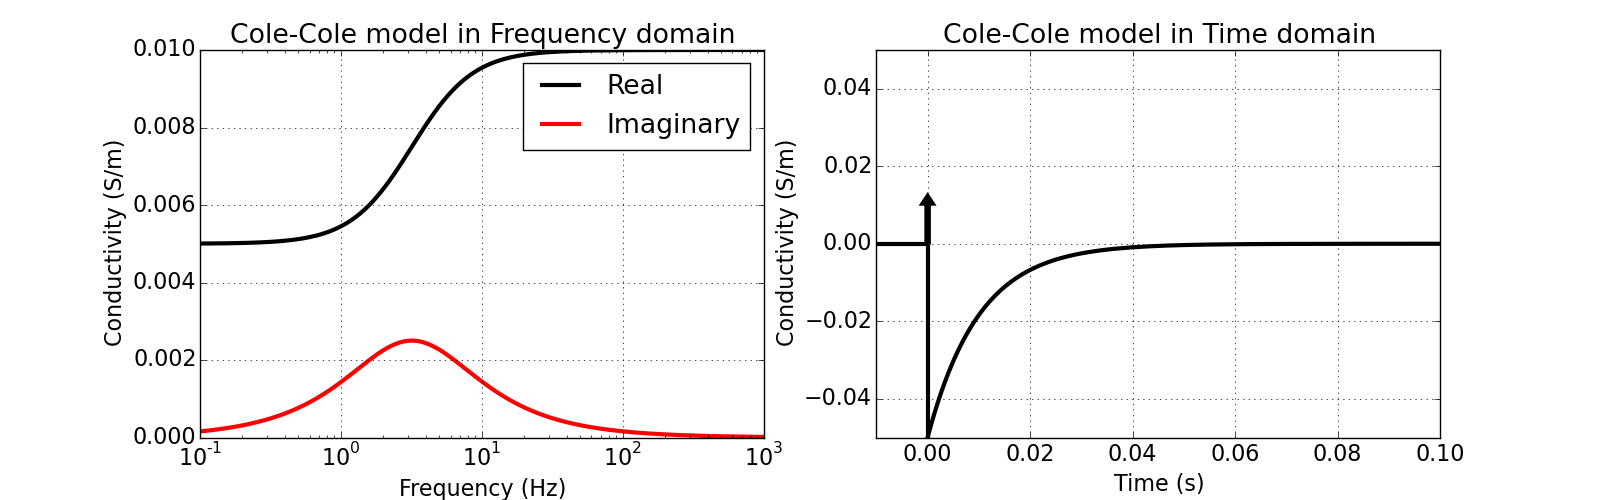
\includegraphics[width=1.0\textwidth]{figures/FDandTDCole.png}
  \caption{Cole-Cole model in frequency domain (a) and time (b) domain. }
  \label{Fig:FDandTDCole}
\end{figure}
\clearpage

%%% ===========================================================================
%%% SECTION 2.2. MAIN
\subsection{Convolution approach}
Consider Maxwell's equations in time domain:
\begin{equation}
  \curl{\e} = -\frac{\partial \b}{\partial t}
  \label{eq: total_farad}
\end{equation}
\begin{equation}
  \curl{\frac{1}{\mu}\b} - \j= \j_{s},
  \label{eq: total_coulomb}
\end{equation}
where $\e$ is the electric field ($V/m$), $\b$ is the magnetic flux density ($Wb/m^2$) and $\mu$ is the magnetic permeability ($H/m$). Here $\j$ is the conduction current. In the frequency domain the current density $\J$ is related to conductivity via $\J(\omega) = \sigma(\omega)\E(\omega)$ where $\E$ is the electric field. Substituting equation (\ref{eq: sigma_freq}) yields:
\begin{equation}
	\J(\omega) = \siginf\E(\omega)+\triangle\sigma(\omega)\E(\omega) =\siginf\E(\omega)+\vec{J}_a(\omega),
\end{equation}
where $\J^a(\omega)$ is the anomalous current density.
Converting this relationship to time domain using a Fourier transform yields:
\begin{equation}
	\j(t) = \sigma(t)\otimes \e(t),
	\label{eq: ohmslaw1}
\end{equation}
where $\otimes$ indicates time convolution. For causal signals, which is defined when $t \ge 0$, convolution between $a(t)$ and $b(t)$ can be written as
\begin{equation}
	a(t) \otimes b(t) = \int_0^t a(u) b(t-u) du.
	\label{eq: convolution}
\end{equation}
That is the current density depends upon the previous history of the electric field. Substituting equation (\ref{eq: sigma_time}) yields:
\begin{equation}
	\j(t) = \siginf\e(t) + \dsig(t)\otimes\e(t) = \siginf\e(t) + \j^a(t),
	\label{eq: ohmslaw2}
\end{equation}
where $\j^a(t) = \dsig(t)\otimes\e(t)$.

As an example consider a chargeable block with the complex conductivity in Figure ~\ref{Fig:ChargeableBlock}, that is subjected to a constant electric field, $\e^{ss}$ at t = 0, and it does not change due to a chargeable body thus $\e(t) = \e^{ss}u(t)$. Due to this, the first term in equation (\ref{eq: ohmslaw2}) can be considered as the current density if there were no polarization effects; the second term are the polarization currents. Following \cite{Smith1988a}, in our system where $\e$ is constant, those can be respectively considered as the fundamental current, $\j^{F}$ and the IP current $\j^{IP}$, which is the same term as $\j^a$. By using Cole-Cole model with $c=1$  and evaluating convolution in the anomalous current density as shown in Figure ~\ref{Fig:Convolution_es}, we have
\begin{equation}
	\j^{IP}(t) = -\eta\siginf [1-e^{-\frac{t}{(1-\eta)\tau}}]\e^{ss} = -\peta(t)\siginf\e^{ss}
	\label{eq: IPdensity}
\end{equation}
with the final value at $t = \infty$ yielding $\j^a=-\eta\siginf\e^{ss}=-\eta\j^F$, and thus $\j = \siginf(1-\eta)\e^{ss}$. That is, the polarization is a fraction, $\eta$ of the fundamental current density, $\j^F$, and is in the opposite direction to $\j^F$. This mathematical representation  about anomalous current density in terms of Cole-Cole model agrees with Seigel's  result (\cite{seigel1959}). Thus, we have total current:
\begin{equation}
	\j(t) = \j^{F}(t) + \j^{IP}(t) = \siginf(1-\peta(t))\e^{ss},
  \label{eq: ohmslaw3}
\end{equation}
where $\peta(t) = \frac{\dsig(t)\otimes u(t)}{\siginf}$.
We can define an effective conductivity as
\begin{equation}
	\sigma_{eff}(t) = \frac{\j(t)}{\e^{ss}} = \siginf(1-\peta(t)) = \siginf + \delta\sigma(t).
  \label{eq: sigeff}
\end{equation}
For $t \rightarrow \infty$, $\peta\rightarrow \eta$ (the intrinsic chargeability) and $\sigma_{eff} = \siginf(1-\eta)$, which is well used result.

Conversely, based on equation (\ref{eq: sigeff}), we define an perturbed conductivity as
\begin{equation}
  \delta\sigma(t) = -\siginf\peta(t) =\frac{\dsig(t)\otimes \e(t)}{\e^{ss}}.
  \label{eq: sigpert}
\end{equation}
Then we can rewrite equation (\ref{eq: ohmslaw3}) as
\begin{equation}
  \j(t) = (\siginf + \delta\sigma(t))\e(t).
\end{equation}
This is a fundamental statement of linearization in time domain electrical field IP (EIP)  and magnetic field IP (MIP) responses, since it allows us to expand Maxwell's operator in terms of $\sigpert(t)$ for each time channel. Although the assumption about constant electric field allows us to have some insights about polarization due to a chargeable body; however, it does not make sense in general cases where we measure time-varying electric field due to the chargeable body. Therefore, this assumption should be released, and will be treated later.


%%% ===========================================================================
%%% SECTION 2.1. FIGURES
\begin{figure}[htb]
  \centering
  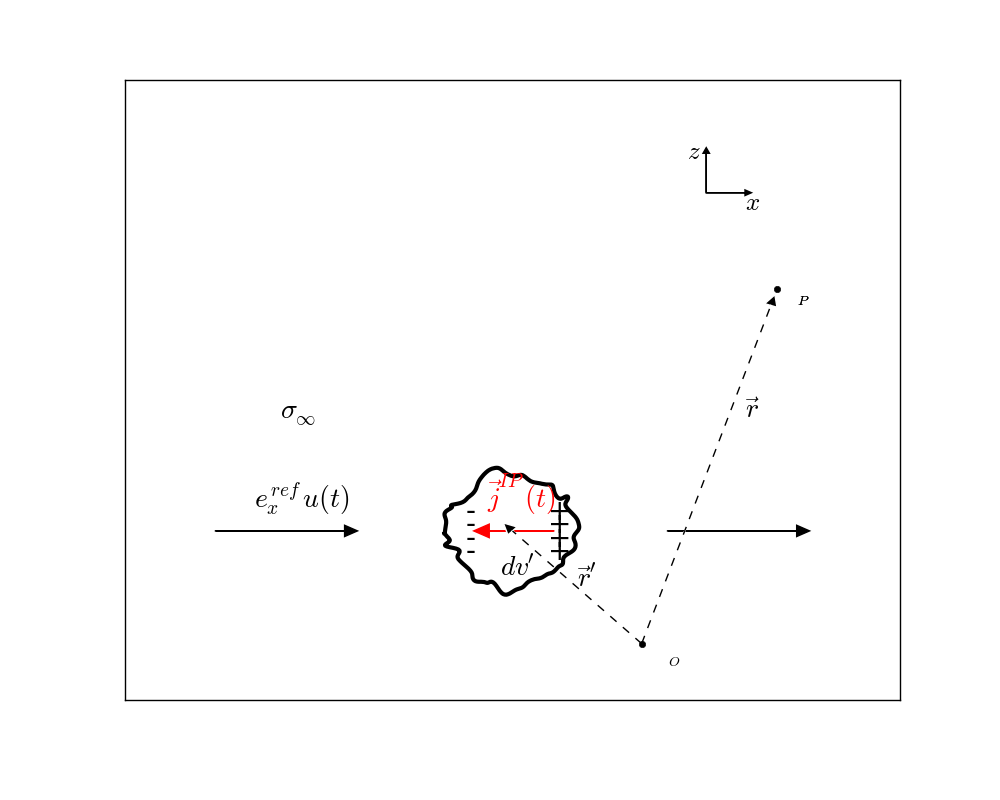
\includegraphics[width=0.6\textwidth]{figures/ChargeableBlock.png}
  \caption{A chargeable block with the complex conductivity, which is subjected to a constant electric field, $\e^{ss}$.}
  \label{Fig:ChargeableBlock}
\end{figure}
\begin{figure}[htb]
  \centering
  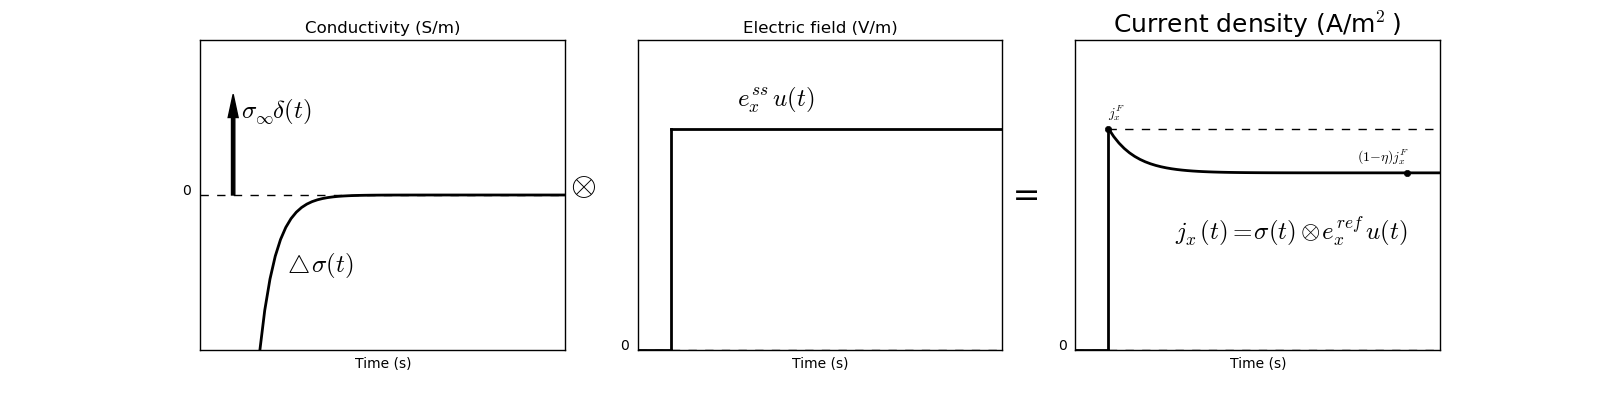
\includegraphics[width=1.0\textwidth]{figures/Convolution_es.png}
  \caption{Convolution of time dependent conductivity ($\sigma(t)$) and step-on electric field in $x$-direction ($e^{ss}_x$). }
  \label{Fig:Convolution_es}
\end{figure}

\clearpage
%%% ===========================================================================
%%% SECTION 2.2. MAIN
\subsection{Decomposition of EM responses}
The basic ideas and notation presented thus far form the foundation of more general cases for grounded and airborne IP measurements. The difference arise because diffusion of the fields into the subsurface need to be taken into account and also electric fields due to polarization can become important. As in \cite{Smith1988a}, we let $\e = \e^{F} + \e^{IP}$, $\b = \b^{F} + \b^{IP}$ and $\j = \j^{F} + \j^{IP}$, where superscript $F$ indicates fundamental and $IP$ is induced polarization.
Substituting into equations (\ref{eq: total_farad}) and (\ref{eq: total_coulomb}) yields the following sequences:
\begin{equation}
  \curl({\e^{F}+\e^{IP}}) = -\frac{\partial}{\partial t} (\b^{F}+\b^{IP}),
\end{equation}
\begin{equation}
  \curl\frac{1}{\mu}(\b^{F}+\b^{IP}) - (\j^{F}+\j^{IP})= \j_{s}.
\end{equation}
By canceling out vectors associated with $EM$ terms, we have
\begin{equation}
  \curl \e^{IP} = -\frac{\partial \b^{IP}}{\partial t},
  \label{eq: eq_secondary_farad}
\end{equation}
\begin{equation}
  \curl{\frac{1}{\mu}\b^{IP}} = \j^{IP}.
  \label{eq: eq_secondary_coulomb}
\end{equation}
In addition, associated $EM$ equations can be written as
\begin{equation}
  \curl \e^{F} = -\frac{\partial \b^{F}}{\partial t},
  \label{eq: eq_primary_farad}
\end{equation}
\begin{equation}
  \curl{\frac{1}{\mu}\b^{F}} -\j^{F} = \j_s.
  \label{eq: eq_primary_coulomb}
\end{equation}
Here
\begin{equation}
  \j^{F}(t) = \siginf\e^{F}(t),
  \label{eq: jF}
\end{equation}
\begin{equation}
  \j^{IP} = \siginf\e^{IP}(t) + \dsig(t)\otimes\e(t).
  \label{eq: jIP}
\end{equation}
Note that IP current density, $\j^{IP}$ is different from the anomalous current density, $\j^a$, which was defined as $\dsig(t)\otimes\e(t)$; $\j^{IP}$ includes the extra term $\siginf\e^{IP}$. This difference induced by the specific system that we have used in convolution approach: constant electric field ($\e(t) = \e^{ss}u(t)$). However, in general system, the equality, $\j^{IP}=\j^a$ is not true, so that the extra term should be considered for $\j^{IP}$.

Let $F[\cdot]$ denote operator associated with Maxwell’s equations and let $d$ denote any electromagnetic field. Keeping same notation, we also write $d = d^{F} + \dip$. Therefore, we define IP datum as
\begin{equation}
	\dip = d - d^{F} = F[\siginf\delta(t)+\dsig(t)]-F[\siginf\delta(t)].
    \label{eq: IPdatum_syn}
\end{equation}
This subtraction process acts as an EM decoupling process, which reduces EM effects to better recognize IP effect in the measured responses. This formed the basics of work by \cite{routh2001}. Thus, assuming that we have reasonable estimation for the distribution of $\siginf$ in 3D space, we can identify  IP datum, which are embedded in the measured responses. We test this assumption with some numerical experiments so that computed $\dip$ responses can transmit meaningful information with even incorrect distribution of $\siginf$.
\bigskip
\todo[inline, color=yellow!40]{
\noindent\textbf{Questions 1: Is it true that we have only IP effect with this subtraction process?} \newline\newline
Doug: We need to show under what circumstances this is true. It is tied in with the statement that $\curl\e^{IP} = 0$. i.e. the polarization decays do not cause EM induction. Handling this matter here simplified much of the following paper.\medskip\newline
\textcolor{blue}{Answer: I think that EM induction due to polarization decays are also IP effect, which is due to time dependent conductivity.}
}
\bigskip
\todo[inline, color=green!20]{
\noindent\textbf{Issue1: Naming issues of $\vec{p}$ and $\j^{IP}$. How about $\j^a$?}
}
%%% ===========================================================================
%%% SECTION 2.4. MAIN
\subsection{Thoughts about $\j^{IP}$ and $\j^a$}
With consideration of time dependent conductivity, current density was written as
\begin{eqnarray*}
    \j(t) = \siginf\e(t)+\j^a(t),
\end{eqnarray*}
where $\j^a(t)=\dsig(t)\otimes\e(t)$. Or this can be rewritten as
\begin{equation*}
    \j(t) = \j^{F}(t) + \j^{IP}(t),
\end{equation*}
where $\j^{F}(t)=\siginf\e^{F}(t)$ and
\begin{eqnarray}
		\j^{IP}(t) = \siginf\e^{IP}(t) + \j^a(t).
        \label{eq: jip_with_ja}
\end{eqnarray}
We first consider anomalous current density $\j_a$. With secondary field formulation shown in equations (\ref{eq: eq_secondary_farad}) and (\ref{eq: eq_secondary_coulomb}), this can be considered as source term. Assuming no EM induction effect, we can have integral equation forms:
\begin{equation}
    \e^{IP}(\vec{r}; t) = \int_{\Omega} \bar{\mathbf{G}}^{E}(\vec{r}, \vec{r}_s)\cdot\j^a(\vec{r}_s; t) dv_s,
\end{equation}
\begin{equation}
    \b^{IP}(\vec{r}; t) = \int_{\Omega} \bar{\mathbf{G}}^{B}(\vec{r}, \vec{r}_s)\cdot\j^a(\vec{r}_s; t) dv_s,
\end{equation}
where $\bar{\mathbf{G}}^{E}$ and $\bar{\mathbf{G}}^{B}$ are electric and magnetic green's tensors. Assuming we know $\j^a$, we can compute $\e^{IP}$ and $\b^{IP}$ by evaluating those integrals. This represents importance of  $\j^a$ for IP responses. In convolution approach $\j^a$ was defined as
\begin{equation}
    \j^a(t) = -\peta(t)\siginf\e^{ss}=-\peta(t)\j^{\ ref},
\end{equation}
where the reference current density is $\j^{\ ref} = \siginf\e^{ss}$.
This allows to build up a conceptual model of IP responses: IP body acts like a dipole which has opposite direction to reference current density, and proportional to $\peta$. This conceptual model is analogous to Seigel's one (\cite{seigel1959}).

Second, we treat IP current density $\j^{IP}$. Based on equation (\ref{eq: eq_secondary_farad}), we can apply Biot-Savart law:
\begin{equation}
  \b^{IP}(\vec{r}; t) = \frac{\mu_0}{4\pi}\int_{\Omega}  \frac{\j^{IP}(\vec{r}_s; t)\times\hat{r}}{|\vec{r}-\vec{r}_s|^2}dv_s,
\end{equation}
thus we can compute $\b^{IP}$ using $\j^{IP}$. Interestingly, this shows we can compute $\b^{IP}$, once we know $\j^{IP}$. Different from magnetic greens tensor, $\bar{\mathbf{G}}^B$, a kernel in Biot-Savart law is purely geometric. However we need to know additional term $\siginf\e^{IP}$ to compute $\b^{IP}$ using Biot-Savart law. This is caused by difference between $\bar{\mathbf{G}}^B$ and kernel function of Biot-Savart law. Both approaches can be useful in spite of some different features.

We have recognized that $\j^{IP}$ can be a fundamental element of understanding IP responses. In order to get some insights of $\j^{IP}$, we rewrite $\j^{IP}$ as
\begin{equation}
    \j^{IP}(t) = \siginf\e^{IP}(t) + \dsig(t)\otimes\e^{F}(t)+ \dsig(t)\otimes\e^{IP}(t).
    \label{eq: jip_three}
\end{equation}
For notational convenience, we respectively refer to $\siginf\e^{IP}(t)$, $\dsig(t)\otimes\e^{F}(t)$ and $\dsig(t)\otimes\e^{IP}(t)$ as $\j^{IP}_1$, $\j^{IP}_2$ and $\j^{IP}_3$. Characteristics of each current density are following. We start with $\j^{IP}_1$. This is defined everywhere. This is the term can be ne, which makes difference between $\j^{IP}$ and $\j^a$. Recalling Smith’s approximate convolution approach (\cite{Smith1988a}), he assumed $\j^{IP}_1$ and $\j^{IP}_3$ are negligible, which makes $\j^{IP} = \j^a$. In his case, a IP body was surrounded by the free space and $\eta \ll 1$.  However, in general case where the background medium is not free space, this term is not negligible in that $\j^{IP}_2$ and $\j^{IP}_3$ are only defined in the IP body because $\dsig(t)$ is zero except for IP body. This shows that $\j^{IP}_2$ is going to be the main term of $\j^{IP}$ in the IP body as the conductivity of background medium and $\eta$ decrease. In addition, $\j^{IP}_3$ might be negligible when we have small $\eta$. However, it is hard to suggest that when we have considerable $\eta$, since this is convoluted property of $\e^{IP}$ and $\dsig(t)$.

%%% ===========================================================================
%%% SECTION 3. MAIN
%%% ===========================================================================
\section{Linearization of IP responses}
%%% ===========================================================================
%%% SECTION 3.1. MAIN
\subsection{Linearization in EIP and MIP}
For our linearization it is useful to think in terms of EIP or MIP experiment where we apply a direct current into the ground. We use step-on waveform. Neglecting induction, $F[\siginf]=F_{DC}[\siginf] \rightarrow \e^{ss}_{\siginf}$, where $F_{DC}[\cdot]$ indicates steady-state Maxwell's operator. Recalling the definitions of $\delta\sigma$ and $\sigma_{eff}$ that we have made in convolution approach, we approximately rewrite total current density, $\j$ as
\begin{eqnarray}
	\j(t) \approx (\siginf + \delta\sigma(t))\e(t) = \sigma_{eff}(t)\e(t).
  	\label{eq: ohmslaw4}
\end{eqnarray}
The perturbed conductivity and effective conductivity were defined as $\delta\sigma = \frac{\dsig(t)\otimes\e(t)}{\e^{ss}}$ and $\sigma_{eff} = \frac{\j}{\e^{ss}}$. Considering that we use step-on waveform, this is reasonable approximation, since $\e(t)\approx \e^{ss}u(t)$ when $\eta \ll 1$. By substituting $\vec{e}^{ss}$ in $\delta\sigma(t)$ with $\vec{e}(t)$, equation (\ref{eq: ohmslaw4}) can be converted to an equality equation. Based on this, by substituting constant electric field $\e^{ss}$ as $\e_{\siginf}^{ss}$, we let
\begin{equation}
  \dsig(t)\otimes\e(t) = \j^a(t) \approx \delta\sigma(t)\e(t)= \frac{\dsig(t)\otimes\e(t)}{\e_{\siginf}}\e(t).
  \label{eq: p_approx}
\end{equation}
% \todo[inline, color=green!20]{
%   \noindent\textbf{
%   Issue2: Not very clear about this statement. What do you think Doug?}\newline
% }
Recall that equation (\ref{eq: ohmslaw4}) suggested us a fundamental characteristic of the EIP problem, since IP response at any time $t>0$ is given by $F_{DC}[\sigma_{eff}(t)]$. Thus, we make Taylor expansion:
\begin{equation}
  F_{DC}[\siginf + \delta\sigma_i] = F_{DC}[\siginf] + \frac{\partial F_{DC}[\siginf]}{\partial\siginf}\delta\sigma_i + O(\delta\sigma_i^2),
  \label{eq: TaylorDC}
\end{equation}
where subscript $i$ indicates $i^{th}$ time channel. By ignoring the second order term in equation (\ref{eq: TaylorDC}) with some linear algebra, therefore, we have IP datum at $i^{th}$ time channel:
\begin{equation}
  \dip_i = F_{DC}[\siginf + \delta\sigma_i] - F_{DC}[\siginf] \approx -\frac{\partial F_{DC}[\siginf]}{\partial log(\siginf)}\peta_i,
  \label{eq: EIPlinear1}
\end{equation}
where $\peta_i = -\frac{\sigpert_i}{\siginf}$. This constructs a general formulation of linear inverse problem in EIP (\cite{Yuval1997}, \cite{Hordt2006}). In addition, this still applicable for MIP by setting the type of $d$ and $F_{DC}$ as magnetic field (\cite{seigel1974}, \cite{Chen2003}).

Conversely, all of our derivations has been done for a step-on current. Then what happen if data are measured in the off-time? This can be treated simply because we can compute off-time data using on-time data, since we have relationship between them as
\begin{equation}
  \dip_{off}(t) = \dip_{on}(t=\infty) - \dip_{on}(t) = F_{DC}[\sigma_0] - \dip_{on}(t),
\end{equation}
where $\sigma_0 = \siginf(1-\eta)$, which is the low frequency limit of Cole-Cole model. This indicates that we can still use equation (\ref{eq: EIPlinear1}), because the off-time result is directly related to the on-time as illustrated in Figure ~\ref{Fig:EIPcurve}. However, in practice, the input current is not step-on or step-off but be arbitrary. We can imagine a current waveform $I_0w(t)$. The maximum charging will occur when a uniform field has been applied for a duration $t \gg \tau$. Let $\e^{ss}$ represents the steady state field associated with $I(t) = I_0u(t)$. In this case, the assumption that we made for $\j^a$ (equation (\ref{eq: p_approx})) may not be reasonable, because the total electric field, $\e(t)$ can dynamically change due to $w(t)$ so that the electric field at $i^{th}$ time channel, $\e_i$ can be quite different from $\e^{ss}$ as shown in Figure ~\ref{Fig:Oscillating_e}. Therefore, for this general waveform, it is not straight forward to linearize EIP responses with the current framework. This will be treated later.

% \todo[inline, color=green!20]{
%   \noindent\textbf{Issue3: I am not sure about this statement}\medskip\newline
%   True $\delta\sigma(t)$ is
%   \begin{equation*}
%     \delta\sigma(t)= \frac{\dsig(t)\otimes \e(t)}{\e(t)}
%   \end{equation*}
%   in which we did not like since it is not well-defined. So, we approximately define
%   \begin{equation*}
%     \delta\sigma(t) \approx \frac{\dsig(t)\otimes \e(t)}{\e^{ss}}.
%   \end{equation*}
%   I think this is okay for step-on case, but if we have oscillating waveform, it is not reasonable assumption. This is because $\e(t)$ should be oscillating as well.

%   Honestly, I still want to put
%   \begin{eqnarray*}
%     \div\j^{IP} = \div \siginf \e^{IP} = -\dsig(t)\otimes \e(t) \\
%     \approx -\dsig(t)\otimes \e^{F}(t).
%   \end{eqnarray*}
%   With $\e^{IP} = \grad \phi^{IP}$, we have
%   \begin{eqnarray*}
%     \phi^{IP}(t) = [\div\siginf\grad]^{-1}(\dsig(t)\otimes \e^{F})\\
%     =-\frac{\partial \phi_{\siginf}}{\partial log (\siginf)}\peta(t),
%   \end{eqnarray*}
%   where $\peta(t) = \frac{\dsig(t)}{\siginf}\otimes w(t)$ and $\phi^{F} = \phi_{\siginf}w(t)$. Once $\dsig(t)\otimes \e^{F}(t) \gg \dsig(t)\otimes \e^{IP}(t)$ holds, this statement is robust, whereas effective conductive way can be easily attacked depending on waveform. This is because the ambiguity in $\delta \sigma(t)$.
% }

%% IE-approach
%%=============
% In addition, using integral equation approach, total electric field can be expressed as
% \begin{equation}
%   \e(t) = \e^{F}+\e^{IP} = \e^{F}+\int_{\Omega} \underline{\mathbf{G}}^E(\vec{r}; \vec{r}_s)\cdot \j^a dv'
% \end{equation}
% where $\underline{\mathbf{G}}^E(\vec{r}; \vec{r}_s)$ is the electric Green's operator with the volumetric integration of $\Omega$ and
% \begin{equation}
%   \e^{IP} = \int_{\Omega} \underline{\mathbf{G}}^E(\vec{r}; \vec{r}_s)\cdot \siginf \e^{ss} \peta (t)dv'.
% \end{equation}
% Since the only time dependent term is $\peta(t)$, we can solve each time channel of EIP problem separately.

%%% ===========================================================================
%%% SECTION 3.1. FIGURE
\begin{figure}[htb]
  \centering
  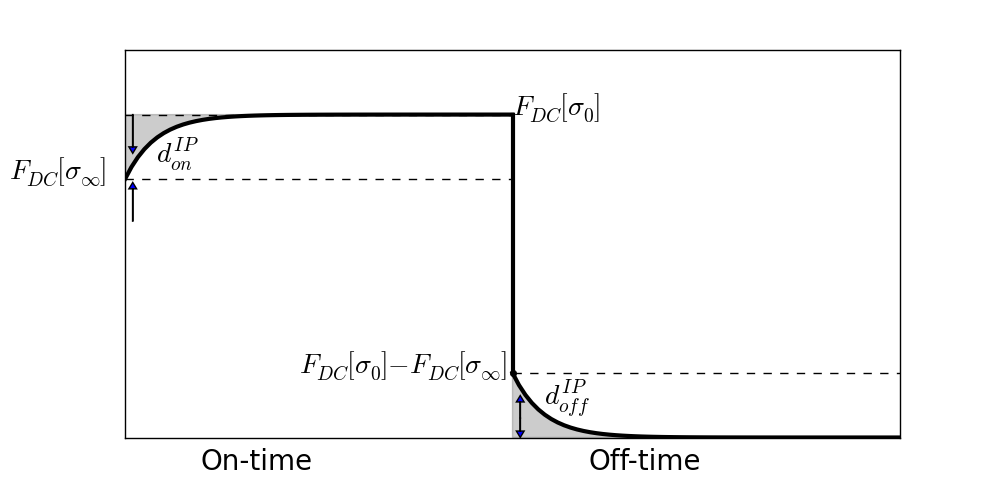
\includegraphics[width=0.8\textwidth]{figures/EIPcurve.png}
  \caption{Time domain EIP curve. }
  \label{Fig:EIPcurve}
\end{figure}
\begin{figure}[htb]
  \centering
  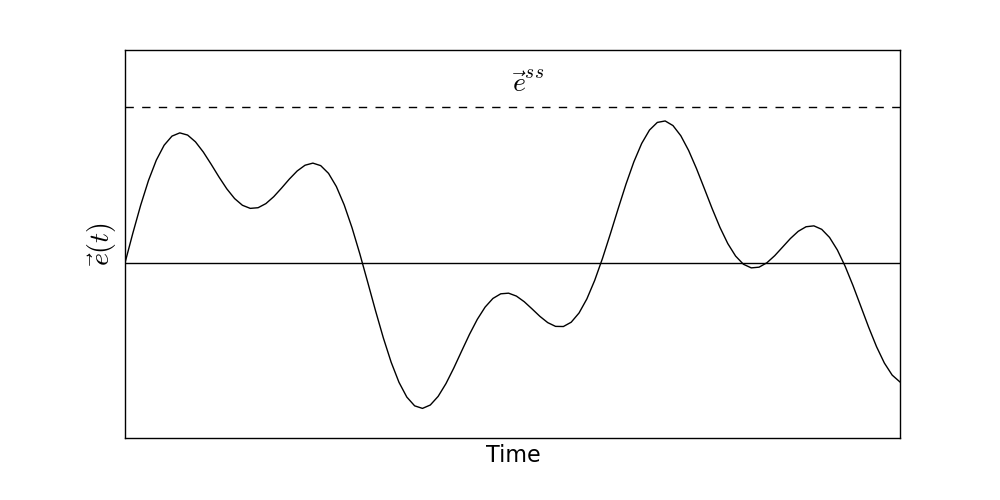
\includegraphics[width=0.8\textwidth]{figures/Oscillating_e.png}
  \caption{Conceptual diagram of oscillating electric field.}
  \label{Fig:Oscillating_e}
\end{figure}
\clearpage

%%% ===========================================================================
%%% SECTION 3.2. MAIN
\subsection{Linearization in EMIP}
In previous two sections, we have treated linearizing IP responses without any EM induction effect. The nice property of EIP and MIP cases was our fundamental responses are time independent, thus, any time dependent responses are due to IP effect. There we assumed that $\frac{\partial \b}{\partial t}\approx 0$. However, in some situations this may not be a reasonable approximation; inductive source TEM can be an extreme example. Therefore, we need to release this assumption to handle those situations where we cannot ignore EM induction effect. Now a principal difference from steady-state IP case is not only fields due to IP effect but also the fundamental fields can be time dependent. However, still, we may want to use similar approach from steady-state case, which expands maxwell's operator in terms of $\sigpert(t)$. A significant problem here is EM induction term ($\frac{\partial \b}{\partial t}$) in equation (\ref{eq: total_farad}). This term makes a coupling between your current and previous time channels, thus expanding this operator in terms of $\sigpert(t)$:
\begin{equation*}
  F[\siginf+\dsig(t)] \approx F[\siginf] + \frac{\partial F[\siginf]}{\partial \siginf}\sigpert
\end{equation*}
is not valid. Accordingly, we need a different approach to tackle this problem, although most of fundamental methodology used in previous cases can be similar in this case.

Nonetheless, our goal is stil quite same as before: we want to express $d^{IP}$ responses as instantaneous property, which is not coupled to previous time channel. Therefore, we can have a form of linear equation like $\dip(t) = -J[\peta(t)]$, where $J[\cdot]$ is a linear operator. For this, we consider a general system whether we can have either grounded or inductive source and any types of measured field. Let total electric field, $\e(t)$ can be written as
\begin{equation}
  \e(t) = \e^{\ ref}w^e(t),
  \label{eq: e_with_eref}
\end{equation}
where $\e^{ref}$ is the reference electric field and $w^e(t)$ is a dimensionless function that prescribes the history of the electric field at each location. $\e^{ref}$ is an appropriate scaling for the electric field, which is independent on time.  Since proper choice of $\e^{\ ref}$ can depend on different types of sources or input current waveform, we do not define $\e^{\ ref}$ here, but this will be treated later. Substituting this into equation (\ref{eq: jIP}) yields
\begin{eqnarray*}
  \j^{IP}(t) = \siginf\e^{IP}(t) + \dsig(t)\otimes w^e(t)\e^{\ ref}
\end{eqnarray*}
and by letting pseudo-chargeability, $\peta(t)$ as
\begin{equation}
    \peta(t) = -\frac{\dsig(t)}{\siginf}\otimes w^e(t),
    \label{eq: pseudochargeability}
\end{equation}
we have
\begin{eqnarray}
  \j^{IP}(t) = \siginf\e^{IP}(t) -\siginf \peta(t)\e^{\ ref}
  \label{eq: jip_EMIP}
\end{eqnarray}
Using Helmholtz decomposition, any electric field, $\e$ can be decomposed as
\begin{equation*}
    \e=-\vec{a}-\grad\phi,
\end{equation*}
where $\vec{a}$ and $\phi$ is electric vector and scalar potentials, respectively and $\div\vec{a}=0$. So, $\e^{IP}$ can be decomposed as
\begin{equation*}
  \e^{IP}=-\vec{a}^{IP}-\grad\phi^{IP}.
\end{equation*}
Now we need to make a core assumption:
\begin{equation}
  \e^{IP} \approx  \e^{IP}_{approx} = -\grad\phi^{IP},
  \label{eq: eip_approx}
\end{equation}
which means $\e^{IP}$ is dominated by galvanic effect ($\frac{\partial\b^{IP}}{\partial t}\approx 0$). Validity of this assumption must be tested for different applications, but now let this assumption is feasible. Nonetheless, let us assume that this is feasible, then this allow us to express $\d^{IP}$ as an instantaneous property.

To show that, we first take $\div$ to equation (\ref{eq: jip_EMIP}) then by substituting  $\e^{IP}$ with equation (\ref{eq: eip_approx}), with some linear algebra we have
\begin{equation}
  \phi^{IP}(t) \approx [\div \siginf\grad]^{-1}\div\siginf\peta(t)\e^{\ ref}.
  \label{eq: phiIPapprox_general}
\end{equation}
By taking $\grad$ to this equation we have
\begin{equation}
    \e^{IP}_{approx} = -\grad[\div \siginf\grad]^{-1}\div\siginf\peta(t)\e^{\ ref}.
    \label{eq: eip_approx_full}
\end{equation}
Thus, we can compute $\e^{IP}_{approx}$, and thus electric field due to IP effect can be expressed as instantaneous fields, which is only dependent on $\peta(t)$ in time.

Some EM instruments measure $\b$ or $\frac{\partial \b}{\partial t}$, so naturally we want to compute $\b^{IP}$ or $\frac{\partial \b^{IP}}{\partial t}$. For this, first we compute $\j^{IP}$ then use Biot-Savart law to compute $\b^{IP}$ or $\frac{\partial \b^{IP}}{\partial t}$. Substituting equation (\ref{eq: phiIPapprox_general}) into equation (\ref{eq: jip_EMIP}), approximated IP current density, $\j^{IP}_{approx}$ can be expressed as
\begin{equation}
  \j^{IP}(t) \approx \j^{IP}_{approx} = -\bar{S}\siginf\e^{\ ref}\peta(t),
  \label{eq: jip_approx}
\end{equation}
where
\begin{equation}
  \bar{S} = -\siginf\grad[\div \siginf\grad]^{-1}\div+\bar{I}
\end{equation}
and $\bar{I}$ is an identity tensor. Then by using Biot-Savart law we have:
\begin{equation}
  \b^{IP}_{approx}(\vec{r}; t) = \frac{\mu_0}{4\pi}\int_{\Omega}  \frac{\bar{S}\e^{\ ref}(\vec{r}_s)\times\hat{r}}{|\vec{r}-\vec{r}_s|^2}\peta(t)dv_s.
  \label{eq: BiotbIP_approx}
\end{equation}
By taking time derivative to the above equation we have
\begin{equation}
  \frac{\partial\b^{IP}_{approx}}{\partial t}(\vec{r}) = \frac{\mu_0}{4\pi} \int_{\Omega}  \frac{\bar{S}\e^{\ ref}(\vec{r}_s)\times\hat{r}}{|\vec{r}-\vec{r}_s|^2}\frac{\partial}{\partial t}\peta(t)dv_s.
  \label{eq: BiotbIPdt_approx}
\end{equation}
Since, the only time dependent term in both equations (\ref{eq: BiotbIP_approx}) and (\ref{eq: BiotbIPdt_approx}) is $\peta(t)$, both $\b^{IP}$ and $\frac{\partial \b^{IP}}{\partial t}$ can be considered as instantaneous fields as well.

To summarize, with the assumption that $\e^{IP}$ is mostly galvanic, we show that electromagnetic fields due to IP effects can be expressed as instantaneous property, which have linear relationship with $\peta(t)$. Therefore, $d^{IP}$ responses, which can be any type of electromagnetic fields, can be represented as $\dip(t) = -J[\peta(t)]$. In discretized space this can be:
\begin{equation}
  \mathbf{d}^{IP}_i = -\mathbf{J}\peta_i,
  \label{eq: dIP_lineareq}
\end{equation}
where $\mathbf{J}$ is corresponding sensitivity matrix and the subscript $i$ indicates $i^{th}$ time channel. Boldface of upper and lower cases indicate a matrix and column vector in discretized space. Since $d^{IP}$ can be any types of electromagnetic fields, our approach to linearize time domain IP responses is applicable for any types of TEM surveys, whereas some details for practical application might be somewhat different. However, the fundamental concept is going to be same.

On the other hand, we must carefully investigate the assumptions that we have made to formulate this linear relationship, and a fundamental characteristics of what we are recovering; thus, we need to identify three fundamental points. We made two assumptions: (a) we know exact background conductivity model ($\siginf$). (b) Inductive effect in $\e^{IP}$ is negligible. In addition, (c) we recognized that $\peta(t)$ is convoluted property with $\e(t)$ and distributed IP parameters. Those three points are not trivial to be validated in physical or mathematical ways; thus each of them should be carefully tested with numerical experiments for different types TEM surveys like grounded or inductive source TEM methods and different background conductivity .

%%% ===========================================================================
%%% SECTION 3.4. MAIN
\subsection{Revisitation of EIP and MIP}
In previous section, we suggested a linearization methodology, which can be applied to general TEM problems. Using this methodology, we revisit linearization of IP responses in EIP and MIP cases. Recall that we have some challenges in linearization when we have general current waveform.

A proper reference electric field, $\e^{\ ref}$ for EIP and MIP cases can be $\e^{ss}_{\siginf}$, so we modify equation (\ref{eq: e_with_eref}) as
\begin{equation*}
    \e(t) = \e^{ss}_{\siginf}w^e(t).
\end{equation*}
Then $\phi^{IP}(t)$ shown in equation (\ref{eq: phiIPapprox_general}), can be rewritten as
\begin{eqnarray*}
  \phi^{IP}(t) = -[\div\siginf\grad]^{-1}\div\grad\phi^{ss}_{\siginf}(\dsig(t)\otimes w^e(t)) \\
               =\frac{\partial \phi^{ss}_{\siginf}}{\partial \siginf}\dsig(t)\otimes w^e(t)
\end{eqnarray*}
and finally we have
\begin{eqnarray}
    \phi^{IP}(t) = \frac{\partial \phi^{ss}_{\siginf}}{\partial \siginf}\dsig(t)\otimes w^e(t) \nonumber\\
                 =\frac{\partial \phi^{ss}_{\siginf}}{\partial \siginf}\sigpert(t)
\end{eqnarray}
where $\sigpert(t) = \frac{\dsig(t)\otimes \e(t)}{\e^{ss}_{\siginf}}=\dsig(t)\otimes w^e(t)$ and
\begin{equation}
    \frac{\partial \phi^{ss}_{\siginf}}{\partial \siginf} = -[\div\siginf\grad]^{-1}\div\grad\phi^{ss}_{\siginf}.
    \label{eq: senseDC}
\end{equation}
Detailed derivation of equation (\ref{eq: senseDC}) in discretized space is given in appendix ??. Substituting equation (\ref{eq: pseudochargeability}) to (\ref{eq: senseDC}), we have
\begin{equation}
    \phi^{IP}(t) = -\frac{\partial \phi^{ss}_{\siginf}}{\partial log(\siginf)}\peta(t),
    \label{eq: phiIPapprox}
\end{equation}
which is the same result from equation (\ref{eq: EIPlinear1}) for electrical potential. Therefore, we can derive same result with conventional linearization in EIP case using suggested methodology. $\e^{IP}$ can also be linearized in the same way, since we can just take gradient to the above equation and obtain $\e^{IP}$.

We also measure magnetic flux density, $\b$, so we similarly linearized $\b^{IP}$ by expanding Maxwell's operator. However, in this time we use different method, which was suggested in previous section. Modifying equation (\ref{eq: jip_EMIP}), we have
\begin{eqnarray}
    \j^{IP}(t) = \siginf\e^{IP}(t) + \dsig(t)\otimes w^e(t)\e^{ss}_{\siginf} \nonumber \\
            = -\bar{S}\siginf\e^{ss}_{\siginf}\peta(t).
\end{eqnarray}
Applying Biot-Savart law yields
\begin{equation}
  \b^{IP}(\vec{r}; t) = \frac{\mu_0}{4\pi}\int_{\Omega}  \frac{\bar{S}\e^{ss}_{\siginf}(\vec{r}_s)\times\hat{r}}{|\vec{r}-\vec{r}_s|^2}\peta(t)dv_s.
  \label{eq: BiotbIP_ss}
\end{equation}
This result shows the applicability of our methodology to MIP. Different from conventional linearization approach used in EIP and MIP cases, applicability of our linearization method is not limited to step-on or step-off waveform, but general. Therefore, even when we have general waveform, which can be oscillating as shown in Figure ~\ref{Fig:Oscillating_e}, the linearzation of EIP or MIP can still proceed. Furthermore, considering an oscillating input current as shown in Figure ~\ref{Fig:Oscillating_e} also supports this statement, because $|\delta(t)| \ll \siginf\eta$.

Interestingly, except ignoring EM induction effect, there is no assumption in our linearization for these EIP and MIP cases so that we can compute exact $\d^{IP}$ responses if we have correct $\peta(t)$. However, we recognize that pseudo-chargeability, $\peta(t)$ is convoluted property between $\e(t)$ and $\dsig(t)$, that is, it is not independent material property, but coupled property with the fields. Then we need to have some insights about $\peta(t)$, since we are going to recover distribution $\peta(t)$, eventually. Assuming $\dsig(t)\otimes \e(t) \approx \dsig(t)\otimes \e^F(t)$, $\peta(t)$ can be modified as
\begin{equation}
    \peta(t) = -\frac{\dsig(t)\otimes w(t)}{\siginf},
\end{equation}
where the input current waveform: $I(t) = I_0w(t)$ and fundamental electric field, $\e^{F} = \e^{ss}_{\siginf}w(t)$. Therefore, $\peta(t)$ is not coupled with the electric field, but with the normalized waveform, $w(t)$. Therefore, pseudo-chargeability can provide meaningful information of distributed IP parameters under our assumption, whereas this assumption should be investigated carefully.
%%% ===========================================================================
%%% SECTION 3.5. MAIN
\subsection{Discussions}

\subsubsection{Choice of $\e^{\ ref}$}
Consider a step-on current waveform with grounded source. Different from EIP or MIP case, here we do not ignore EM induction effect, therefore, even fundamental responses are coupled with time, that is, responses at current time channel are dependent on previous time channel. In spite of this difference, initial and final responses, which respectively refer $\lim_{t\rightarrow 0}d (t)$ and $\lim_{t\rightarrow \infty}d (t)$, are going to be same as EIP case as shown in Figure (\ref{Fig:EIPcurve}). A fundamental difference may be induced by $\e^F(t)$, since it contains not only DC responses, but also EM induction effect: $\e^F(t) = \e^{ss}_{\siginf}u(t)+\e^{EM}(t)$. Since both term generates IP effect, we need to identify which one is dominant term. This may not be easy, since the second term can have arbitrary time decaying feature based on the conductivity distribution of the earth. Nonetheless, if the first term is dominant for all time channels, then it is reasonable to choose $\e^{ss}_{\siginf}$ as $\e^{\ ref}$, which is same as EIP case. In contrast, if the second term is dominant, an intuitive choice can be $\e^{F}_{max} = \e^{F}(t) \otimes \delta(t-t^{max})$, where
\begin{equation}
  \e^{F}_{max} = \e^{F}(t) \otimes \delta(t-t^{max}),
\end{equation}
where $t^{max}$ is the time when the magnitude of fundamental electric fields reach to the maximum. Note that $t_{max}$ is variable in 3D space, since electric field at each pixel in 3D space can have different time decaying feature due to the source location and conductivity distribution.

A fundamental difference from galvanic and inductive source arises from the property, $\div\j_s$.  If this is zero then it is inductive source or if not, it is galvanic source. In order to get some insight, consider DC problem for inductive source:
\begin{eqnarray*}
    -\div\j^{ss} = \div\j_s = 0, \\
    \div \siginf \grad \phi^{ss}_{\siginf} = -\div\j_s = 0.
\end{eqnarray*}
Since the right-hand side of the above equation is zero, thus, $\phi^{ss}_{\siginf}$ = 0 and $\e^{ss}_{\siginf}=0$. This shows that there are no DC fields for inductive source case so that we have $\e^{F} = \e^{EM}$. Then natural choice of $\e^{\ ref}$ is going to be $\e^{F}_{max} = \e^{EM}_{max}$. Now,Consider a step-off waveform, which might more proper for inductive source case. After the current source switch off, electric field starts to increase (may be oscillating)
from zero, and reaches at the maximum, then decays. Therefore, we recognize that $\e^{F}_{max}$ as $\e^{\ ref}$ for inductive source case is reasonable.

\subsubsection{$\frac{\partial \b^{IP}}{\partial t}\approx 0$ is reasonable?}

In constrolled-source EM (CSEM) experiments, we can have two types of sources: grounded and inductive sources. We first consider this assumption for grounded source. Ignoring inductive part of IP effect $\frac{\partial \b^{IP}}{\partial t}\approx 0$, might be okay for grounded source case, since galvanic effect  can be dominant ($\grad\phi^{IP} \gg \vec{a}^{IP}$) in most cases, but this should be carefully tested since it depends on which background conductivity model we have. For example, if we have really conductive background, then $\vec{a}^{IP}$ can be significant compared to $\phi^{IP}$.

For inductive source case, one might think this assumption may not be reasonable, since EM induction is the main driving force of the system, which is the principal difference from grounded source. However, this assumption can be reasonable even in inductive source. Consider a situation where we have homogeneous background conductivity model. Recall $\j^{IP}$ with Helmholtz decomposition:
\begin{eqnarray*}
    \j^{IP} = \siginf\e^{IP} + \dsig(t)\otimes w^{e}(t)\e^{\ ref} \\
            = -\siginf(\grad\phi^{IP}+\vec{a}^{IP}) + \dsig(t)\otimes w^{e}(t)\e^{\ ref}
\end{eqnarray*}
By taking $\div$ we have
\begin{equation*}
    -\div\siginf\grad\phi^{IP}-\div\siginf\vec{a}^{IP} = -\div\dsig(t)\otimes w^{e}(t)\e^{\ ref}.
\end{equation*}
Since $\siginf$ is constant in space, then we rewrite
\begin{equation*}
    \div\siginf\grad\phi^{IP} = \div\dsig(t)\otimes w^{e}(t)\e^{\ ref},
\end{equation*}
where $\div\vec{a}^{IP}=0$ . Therefore, once we do not have any conductivity variation in our background conductivity model, we can have reasonable $\phi^{IP}$. This indicates we can compute IP responses, which are related to galvanic effect, while we still can have significant induction portion, $\vec{a}^{IP}$ in $\e^{IP}$. Note that $\div\vec{a}^{IP}=0$ does not mean $\vec{a}^{IP}=0$. Intuitively, we know that EM induction effect is going to decay faster than galvanic effect so that they are going to small in late time channels. To consider this, we consider Faraday's law
\begin{eqnarray*}
    \curl \vec{a}^{IP}(t) = \frac{\partial \b^{IP}(t)}{\partial t},
\end{eqnarray*}
since $\curl \grad \phi^{IP} = 0$. In frequency domain this can be written as
\begin{equation*}
    \curl \vec{A}^{IP}(\omega) = \imath\omega\B^{IP}(\omega).
\end{equation*}
This tells us time varying magnetic flux density generate rotational electric field, that is $\vec{a}^{IP}$. And the magnitude of that induced field is proportional to $\omega$ in frequency domain. As $\omega$ decrease, EM induction effect gets smaller. Accordingly, $\vec{a}^{IP}$ in $\e^{IP}$ gets smaller as we move on to late time channels, thus galvanic term $\phi^{IP}$ can be dominant term in $\e^{IP}$ at certain late time channels. Those are possible situations that we are interested for IP signals and we might have some chances to apply our linearization methodology.

\bigskip
\todo[inline, color=yellow!40]{
\noindent\textbf{Issue2: What is dominant term in $\e^{\ ref}=\e^{EM}_{max}$?: }
\medskip\newline
\textcolor{blue}{Answer: this should be $\vec{a}^{EM}_{max}$.}
}

% which can be used in actual paper
%==============================================================================
% Due to the consideration of time dependent conductivity, current density includes convolution term (\ref{eq: ohmslaw1}), and this can make significant complexity in computing forward response of this EM system. Intuitively, inverse problem to recover distribution of time dependent conductivity can also be much more complex. Although we can directly derive inverse problem to recover 4D distribution of time dependent conductivity or distributed Cole-Cole parameters; however, we choose a linearization approach to simplify this inverse problem. Based on the experience in DC-IP inversion in  the past couple decades, we believe that the linearization approach can be a more robust solution to approach this inverse problem.

% Principal flow of linearization of time domain IP responses for inductive source has two steps: (a) The most principal component of our linearization is polarization current density, $\j^{IP}$. We linearize $\j^{IP}$ and express in terms of pseudo chargeability.  (b) Once we have $\j^{IP}$ then $\b^{IP}$ of $\frac{\partial\b^{IP}}{\partial t}$ can be computed using Biot-Savart law. Recalling that measured data for inductive source are $\b$ or $\frac{\partial\b}{\partial t}$, TEM responses can be linearized as a function of pseudo-chargeability.

% where $t^{max}$ is the time when the magnitude of fundamental electric fields reach to the maximum. Note that $t_{max}$ and $w(t)$ are variable in 3D space, since electric field at each pixel in 3D space can have different time decaying feature due to Tx-Rx configuration and background conductivity.

% Conversely, we consider that we measure $\b$ or $\frac{\partial \b}{\partial t}$ when we use inductive source for time domain EM survey. Given that we know how to compute $\j^{IP}$, we use Biot-Savart law to compute $\b^{IP}$ and $\frac{\partial\b^{IP}}{\partial t}$:

% Following the notation in \cite{Smith1988a}, we rewrite equation(\ref{eq: ohmslaw2}) as
% \begin{equation}
% 	\j = \j^{F}  + \j^{IP},
% \end{equation}
% where $\j^F$ is the fundamental current density if there were no polarization effects, and $\j^{IP}$ is the IP current density. In the same manner, $\e$ can be decomposed as $\e^{F}+\e^{IP}$, thus we have $\j^{F} = \siginf\e^{F}$ and $\j^{IP} = \siginf\e^{IP}+\dsig(t)\otimes\e(t)$.

% Therefore, in the end, by substituting equation (\ref{F: jip_approx}) to equations (\ref{F: BiotbIP}) and (\ref{F: BiotbIPdt}), we can set a linear inverse problem, which restore each time channel of $\peta(t)$, separately. For this, it is important that we need to know 3D distribution of $\siginf$, which is not trivial in practice. However, we have some chances that we can restore reasonable $\siginf$ distribution by applying 3D inversion to the measured ATEM data with exception of significantly contaminated data by IP effect (CITEyang2014).

\clearpage
%%% ===========================================================================
%%% SECTION 4. MAIN
%%% ===========================================================================
\section{IP inversion methodology}
\subsection{IP inversion procedure}

Application of our linear inversion approach can be divided to main steps. First we identify $d^{IP}$ responses using equation (\ref{eq: IPdatum_syn}), then apply linear inversion to restore distribution of pseudo-chargeability. However, in practice there can be some challenges that we need to over come in both steps. Therefore, we suggest a procedure of TEM-IP inversion.

To obtain the fundamental EM response, $d^F$, (a) invert ATEM data and recover a 3D conductivity model. This may involve omitting data that are obviously contaminated
with IP signals, such as the existence of negative transients in coincident loop surveys. (b)Forward modelling then yields an approximate value of $d^F$ and subtract it from the observations, $d^{obs}$. However, we cannot get the correct $d^F$, since the estimated background conductivity is not exact. (c) Therefore the computed $d^{IP}$ data may contain a residual field due to the incorrect background conductivity. We assume this residual field is a large-scale smoothly varying perturbation to the $d^{IP}$ data and refer to it as regional field. To estimate it, we fit the computed $d^{IP}$ data with a low order polynomial and subtract that from the $d^{IP}$ data. This regional removal process can be expressed as
\begin{equation}
    d^{IP} = d^{obs} - d[\sigma_{est}] - \delta d = raw \ d^{IP} -  \delta d,
\end{equation}
where $\sigma_{est}$ is the background conductivity model estimated from 3D ATEM inversion, $d[\sigma_{est}]$ is the forward modelled data from $\sigma_{est}$, and $\delta d$ arises from the regional processing. Here we let $raw \ d^{IP}= d^{obs}- d[\sigma_{est}]$. (d) The final data are linearly related to a pseudo-chargeability through a sensitivity function shown in equation (\ref{eq: dIP_lineareq}). (e) The $\dip$ at various time channels can be inverted individually. The pseudo-chargeability models may be useful in themselves or they may be further processed to estimate Cole-Cole, or equivalent parameters.

\subsection{Discretization of linear IP problem}
In order to restore distributed $\peta(x, y, z; t)$ in 4D space, first we need to discretize Biot-Savart law shown in equations (\ref{eq: BiotbIP_approx}) and (\ref{eq: BiotbIPdt_approx}). In addition, based on the discretization that we choose, we need to compute $\e^{F}_{max}$. In our discretization $\j^{IP}$ and  $\tilde{\eta}_w$ are defined on the cell center, and those for each time channel are constant in a cell volume, whereas $\e^{F}_{max}$ is defined on the cell edges. We define the number of cells and edges in 3D space as nC and nE, respectively. Assuming we have discretized IP current densitivity distribution ($\dj^{IP}_{cc}$), which has dimension: [(3nC)$\times$1] and defined on the cell center, since $\j^{IP}$ has three components, we first discretize integration operator including cross product ($\int_{v}\frac{ \times \hat{r}}{r^2}dv$) as
\begin{equation}
  \mathbf{G}_{Biot} =
  \begin{bmatrix}
       \mathbf{e}^T &  \mathbf{0}   & \mathbf{0}  \\
       \mathbf{0}   &  \mathbf{e}^T & \mathbf{0}  \\
       \mathbf{0}   &  \mathbf{0}   & \mathbf{e}^T
    \end{bmatrix}
  \begin{bmatrix}
       \mathbf{0}     &   \mathbf{S}_z   & -\mathbf{S}_y  \\
      -\mathbf{S}_z   &   \mathbf{0}     &  \mathbf{S}_x  \\
       \mathbf{S}_y   &  -\mathbf{S}_x   &  \mathbf{0}
    \end{bmatrix},
 \end{equation}
where
\begin{eqnarray*}
  \mathbf{S}_i =\diag(\mathbf{r}_i \oplus \frac{1}{\mathbf{r}^2}), \ i = x, \ y, \ z
\end{eqnarray*}
and $\mathbf{e}$ is a column vector of which element is 1 and has the dimension: [nC$\times$1], $\diag(\cdot)$ is the diagonal matrix and $\oplus$ is the Hadamard product. Then we consider discrete expression for $\j^{IP}$ shown in equation (\ref{eq: jip_approx}), and modify this equation as
\begin{eqnarray}
  \dj^{IP}_{cc}(t) = -\mathbf{S}\diag(\de^{F}_{max})\Ace^T\diag(\vol)\diag(\siginf)\peta(t),
\end{eqnarray}
where
\begin{eqnarray}
  \mathbf{S} = \mathbf{A}^{e}_{ccv}\Me^{-1}[-\MeSigInf \mathbf{G} \A_{\siginf}^{-1}\mathbf{G}^T + \mathbf{I}] \diag(\de^{F}_{max})\Ace^T\diag(\vol)\diag(\siginf).
\end{eqnarray}
and $\mathbf{A}^{e}_{ccv}$ is discrete averaging matrix from edge to cell center with consideration of three component vector so that dimension of this matrix is [3nC$\times$nE]. Thus, we can have linear equation for $k^{th}$ time channel as
\begin{eqnarray*}
  \db^{IP}_k = -\Gbiot \mathbf{S} \peta_k,
\end{eqnarray*}
where sub-index $k$ indcates $k^{th}$ time channel. Finally, by letting
\begin{equation}
  \mathbf{J} = -\Gbiot\mathbf{S},
  \label{eq: Sense}
\end{equation}
we have
\begin{eqnarray}
  \db^{IP}_k = -\mathbf{J}\peta_k,
  \label{eq: bIP_linear}
\end{eqnarray}
where $\mathbf{J}$ is the Jacobian matrix of the linear equation, and since $\mathbf{J}$ is not time-dependent we also have
\begin{eqnarray}
  \frac{\partial\db^{IP}_k}{\partial t} = -\mathbf{J}\frac{\partial}{\partial t}\peta_k.
  \label{eq: dbIPdt_linear}
\end{eqnarray}
Therefore, we can restore distributed $\peta(t)$ or $\frac{\partial}{\partial t}\peta(t)$ based on the data type we have. Note that problems shown in equations (\ref{eq: bIP_linear}) and (\ref{eq: dbIPdt_linear}) are linear problems; thus, by solving linear inverse problem for each time channel we can recover distributed IP parameters. Detailed description about discrete operators are shown in Appendix ??.


\subsection{Linear inversion}
To set up an linear inverse problem we rewrite equation (\ref{eq: dIP_lineareq}) as
\begin{eqnarray}
  \mathbf{d}^{pred} = \mathbf{A}\mathbf{m},
  \label{eq9}
\end{eqnarray}
where $\mathbf{A}$ is sensitivity matrix of linear problem, which corresponds to $\mathbf{J}$ shown in equation (\ref{eq: dIP_lineareq}), $\mathbf{d}^{pred}$ is IP responses at $k^{th}$ time channel ($\mathbf{d}^{IP}_k$), $\mathbf{m}$ is distributed model parameters, which can be either $\peta_{k}$ or $\frac{\partial}{\partial t}\peta_{k}$. This presents that we invert each time channel of $d^{IP}$, separately. Our inversion methodology is based upon that described in \cite{doug1994}. The solution to the inverse problem is the model $\mathbf{m}$ that solves the optimization problem
\begin{eqnarray}
  minimize \ \phi =  \phi_d(\mathbf{m}) + \phi_m(\mathbf{m})\nonumber \\
  s.t. \ 0 \le \mathbf{m},
  \label{eq10}
\end{eqnarray}
where $\phi_d$ is a measure of data misfit, $\phi_m$ is a user defined model objective function and $\beta$ is regularization or trade-off parameter. We use the sum of the squares to measure data misfit
\begin{eqnarray}
  \phi_d = \| \mathbf{W_d}(\mathbf{A}\mathbf{m}-d^{obs}|)\|^2_2 =
  \sum^N_{j=1}(\frac{\mathbf{d}^{pred}_j-\mathbf{d}^{obs}_j}{\epsilon_j}),
  \label{eq11}
\end{eqnarray}
where $N$ is the number of the observed data and $\mathbf{W_d}$ is a diagonal data weighting matrix which contains the reciprocal of the esitmated uncertainty of each datum (
$\epsilon_j$) on the main diagonal,  $\mathbf{d}^{obs}$ is a vector containing the observed data, $\mathbf{d}^{pred}$ is a vector containing calculated data from a linear equation given in equation (\ref{eq9}).
The model objective function, $\phi_m$ is a measure of amount structure in the model and, upon minimization, will generate a smooth model which is close to a reference model, $m_{ref}$. We define $\phi_m$ as
\begin{eqnarray}
  \phi_m = \alpha_s\| \mathbf{W}_s\mathbf{W}(\mathbf{m}-\mathbf{m}_{ref})\|^2_2+
       \alpha_x\| \mathbf{W}_x\mathbf{W}(\mathbf{m}-\mathbf{m}_{ref})\|^2_2+ \nonumber \\
       \alpha_y\| \mathbf{W}_y\mathbf{W}(\mathbf{m}-\mathbf{m}_{ref})\|^2_2+
       \alpha_z\| \mathbf{W}_z\mathbf{W}(\mathbf{m}-\mathbf{m}_{ref})\|^2_2,
  \label{eq12}
\end{eqnarray}
where $\mathbf{W}_s$ is a diagonal matrix, and $\mathbf{W}_x$, $\mathbf{W}_y$ and $\mathbf{W}_z$ are discrete approximations of the first derivative operator in $x$, $y$ and $z$ directions, respectively.  The $\alpha$'s are weighting parameters that balance the relative importance of producing small or smooth models. Model weighting matrix, $\mathbf{W}$ is defined as
\begin{equation}
    \mathbf{W} = \mathbf{diag}(\mathbf{w}),
    \label{eq: weight_mat}
\end{equation}
where $\mathbf{w}$ is a column vector for weighting each model parameters.
%%% ===========================================================================
%%% SECTION 5. MAIN
%%% ===========================================================================
\section{Application: ATEM}

In order to investigate the suggested methodolgies to restore distributed IP parameters from $d^{IP}$ responses in ATEM problem, we compose an IP body model, which includes IP body in the half-space as shown in Figure~\ref{F: IPModel}. Cole-Cole parameters of this IP body are fixed to $\eta=0.2$, $\tau=0.005$ and $c=1$. Conductivity value of the half-space, ($\sigma_{half-space}$) is fixed to $0.001$ S/m, whereas $\siginf$ for the IP body varies. We have two different model, where we named canonical ($\siginf=\sigma_{half-space}$) and conductive ($\siginf=10^2\times\sigma_{half-space}$) models.   For the discretization of 3D earth, $50\times50\times50$ m core cell is used and the number of cell in the domain is $41\times41\times40$. The size of the IP body is $250\times250\times250$ m and the top boundary of this IP body is located at $50$ m below the surface. In order to generate synthetic ATEM-IP data, we use EMTDIP code developed by \cite{marchant2012a}

Survey geometry include 11 stations in each 11 lines as shown in Figure \ref{F: IPModel}a so that we have 121 stations. We use coincident-loop system and both Tx and Rx are located 30 m above the surface; radius of the loop is 10 m. Step-off transmitter waveform is used and the range of the observed time channel is 0.01-10 ms. Measured response is vertical component of $\frac{\partial\b}{\partial t}$. Based on this set up, in this section, first we identify $d^{IP}$ embedded in ATEM responses and analyze characteristics of them. Then we discuss the possibility of the regional due to the inexact background conductivity model in practice. Second, we validate fundamental approximations in our linearization idea by comparing $\j^{IP}$ and $\j^{IP}_{approx}$. Based on this validation, third, we apply linear inversion to each time channel of $d^{IP}$ data separately and restore 3D distribution of $\tilde{\eta}$ for each time channel. We also evaluate this restored distribution of $\peta$ for each time channel, to answer whether this convoluted property with electric fields can provide us meaningful information of distributed IP parameters of the earth. Finally, we investigate effect of inexact $\siginf$ model in the inversion.

\begin{figure}[htb]
  \centering
  % 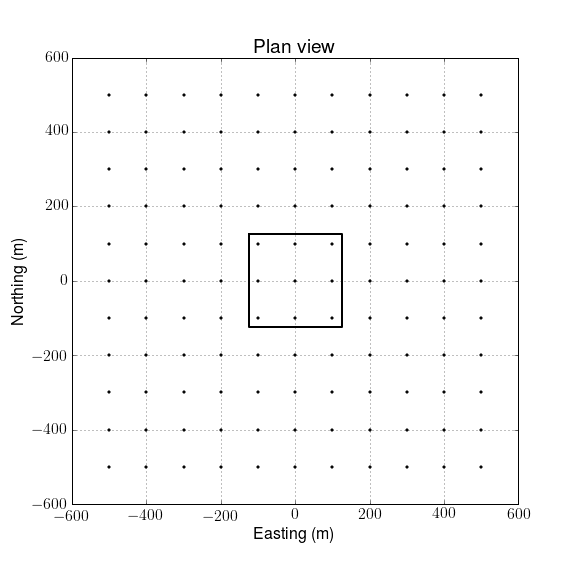
\includegraphics[width=0.5\textwidth]{../figures/syntheticex/Planview.png} \\
  (a) \\
  % 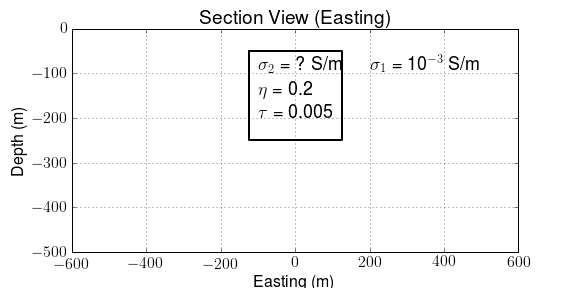
\includegraphics[width=0.5\textwidth]{../figures/syntheticex/Sectionview.png} \\
  (b)
  \caption{Planal (a) and sectional (b) views of IP model. Dashed line in (a) contours the boundary of the IP body. Solid circles in (a) denotes the location of stations.}
  \label{F: IPModel}
\end{figure}
\clearpage

\subsection{Analyses of ATEM-IP responses}
Identification of $d^{IP}$ data, which can be embedded in observed data, is the first step of ATEM-IP inversion. Sometimes, this can be obvious. For example, negative transients of $\frac{\partial b_z}{\partial t}$ responses from coincident loop system can be a clear signature of IP signals. However, we usually observe this in relatively late time channels, which implies that in early time channels we can have dominant EM coupling since we have small IP effect. Even we can face some challenging situations where we do not observe negative transients, and if we use different configuration from coincident loop then identification of IP signals are not trivial. For this, we use EM decoupling method shown in equation (\ref{eq: IPdatum_syn}).

In order to investigate performance of this EM decoupling procedure, we use two different models: canonical and conductive. First we treat canonical model, where $\siginf$ of the IP body is same as $\sigma_{half-space}$. Assuming that we know the true background conductivity model, $\siginf$, we computed $\frac{\partial b_z}{\partial t}$ responses of $d$, $d^F$ and $d^{IP}$ data at the sounding locations. We present those at t=0.37 and t=4.7 ms in Figures ~\ref{F: EMIPresp1_case1} and ~\ref{F: EMIPresp2_case1}, respectively. In Figure ~\ref{F: EMIPresp1_case1}a and ~\ref{F: EMIPresp2_case1}a, we present time decaying curves for both simulations at sounding location at 0 m  easting  and 0 m northing. Black and blue lines respectively indicate $d$ and $d^F$. In addition, we present all of synthetic responses with given survey geometry in Figures ~\ref{F: EMIPresp1_case1}b and ~\ref{F: EMIPresp2_case1}b, and the northing profile at center line on top-right panels. Since there are no conductivity contrast between half-space and IP body. We do not observe any spatial variation in $d$ and $d^F$ at t=0.37 ms as shown in Figure ~\ref{F: EMIPresp1_case1}b. However, in later time channel, t=4.7 ms, we can observe some variations in $d$ (Figure ~\ref{F: EMIPresp2_case1}), which are due to IP effect. We recognize that even in later time channels, we do not have any negative transients so that it is hard for us to recognize $d^{IP}$ responses just by looking the observed data. By subtracting $d^F$ from $d$, we compute $d^{IP}$. With this EM decoupling process we can effectively reduces EM coupling and cleary recognize $d^{IP}$ responses.

Second, we consider conductive model of which $\siginf$ of IP body is $10^2$ time larger than $\sigma_{half\text{-}space}$. In Figure ~\ref{F: EMIPresp2_case1}b, we observe significant anomalous responses in both $d$ and $d^{F}$ at t=0.37 ms due to this conductivity contrast between IP body and half-space. In addition, it is hard to identify IP effect, which are embedded in $d$. However, we can cleary recognize $d^{IP}$ responses through the subtraction process. Different from canonical model, in later time channel, t=4.7 ms, we can observe negative transients as shown in left panel of Figure ~\ref{F: EMIPresp2_case2}b. We have shown that we can better identify IP effect by computing $d^{IP}$ responses with two different models. Even we recognize that we can detect IP responses, which we did not see in the observed data with the EM decoupling process.

Conversely, since we have two different model where the only difference is $\siginf$ of the IP body, we investigate some features in $d^{IP}$ responses for these models. As shown in time decaying curves for both models (left panels of Figure \ref{F: EMIPresp1_case1}a and \ref{F: EMIPresp1_case2}a), $d^F$ are always positive in both cases. $d^{IP}$ responses always have opposite sign to $d^F$ except some early time channels. This is nice property that we need to identify when we process the measured data to compute $d^{IP}$ in practice. Relative strength of $d^{IP}$ responses to $d^F$ is greater with conductive model than those with canonical model which indicate that we may have more possibility to see negative transients for conductive IP body. In addition, as shown in the right panel of Figures \ref{F: EMIPresp2_case1}b and \ref{F: EMIPresp2_case2}b, $d^{IP}$ responses for canonical model has broader distribution than those for conductive model.

We assumed that we know correct 3D distribution of the background conductivity model to compute $d^{IP}$ responses. However, in practice, we may not know the exact background conductivity model, whereas we can have some chances that we can restore reasonable background conductivity model by inverting ATEM data with exception of severely IP contaminated data. To investigate this, first we choose conductive model case and generated $d^{IP}$ data using incorrect background conductivity models, $2\siginf$ and $0.5\siginf$. We chose conductive model since this might be more affected by incorrect background conductivity model. In Figure ~\ref{F: Regionalresp_case2}a, we presented $d^{IP}$ responses for all sounding locations at t=4.2 ms, and we also present northing profile of $d^{IP}$ responses  at the center line in Figure ~\ref{F: Regionalresp_case2}b.  Compared to $d^{IP}$ from the correct conductivity model, data from incorrect conductivity models are biased. $d^{IP}[0.5\siginf]$ shows higher magnitude than $\dip[\siginf]$, whereas $\dip[2\siginf]$ has smaller magnitude than $\dip[\siginf]$. This example shows the potential need of estimating a regional field ($\delta d$) and subtracting it from EM decoupled data. For relatively late time channels where we have considerable IP effect compared to EM coupling, we can ignore positive $d^{IP}$ data since we already recognized that $d^{IP}$ responses are commonly negatives.




\begin{figure}[htb]
  \centering
  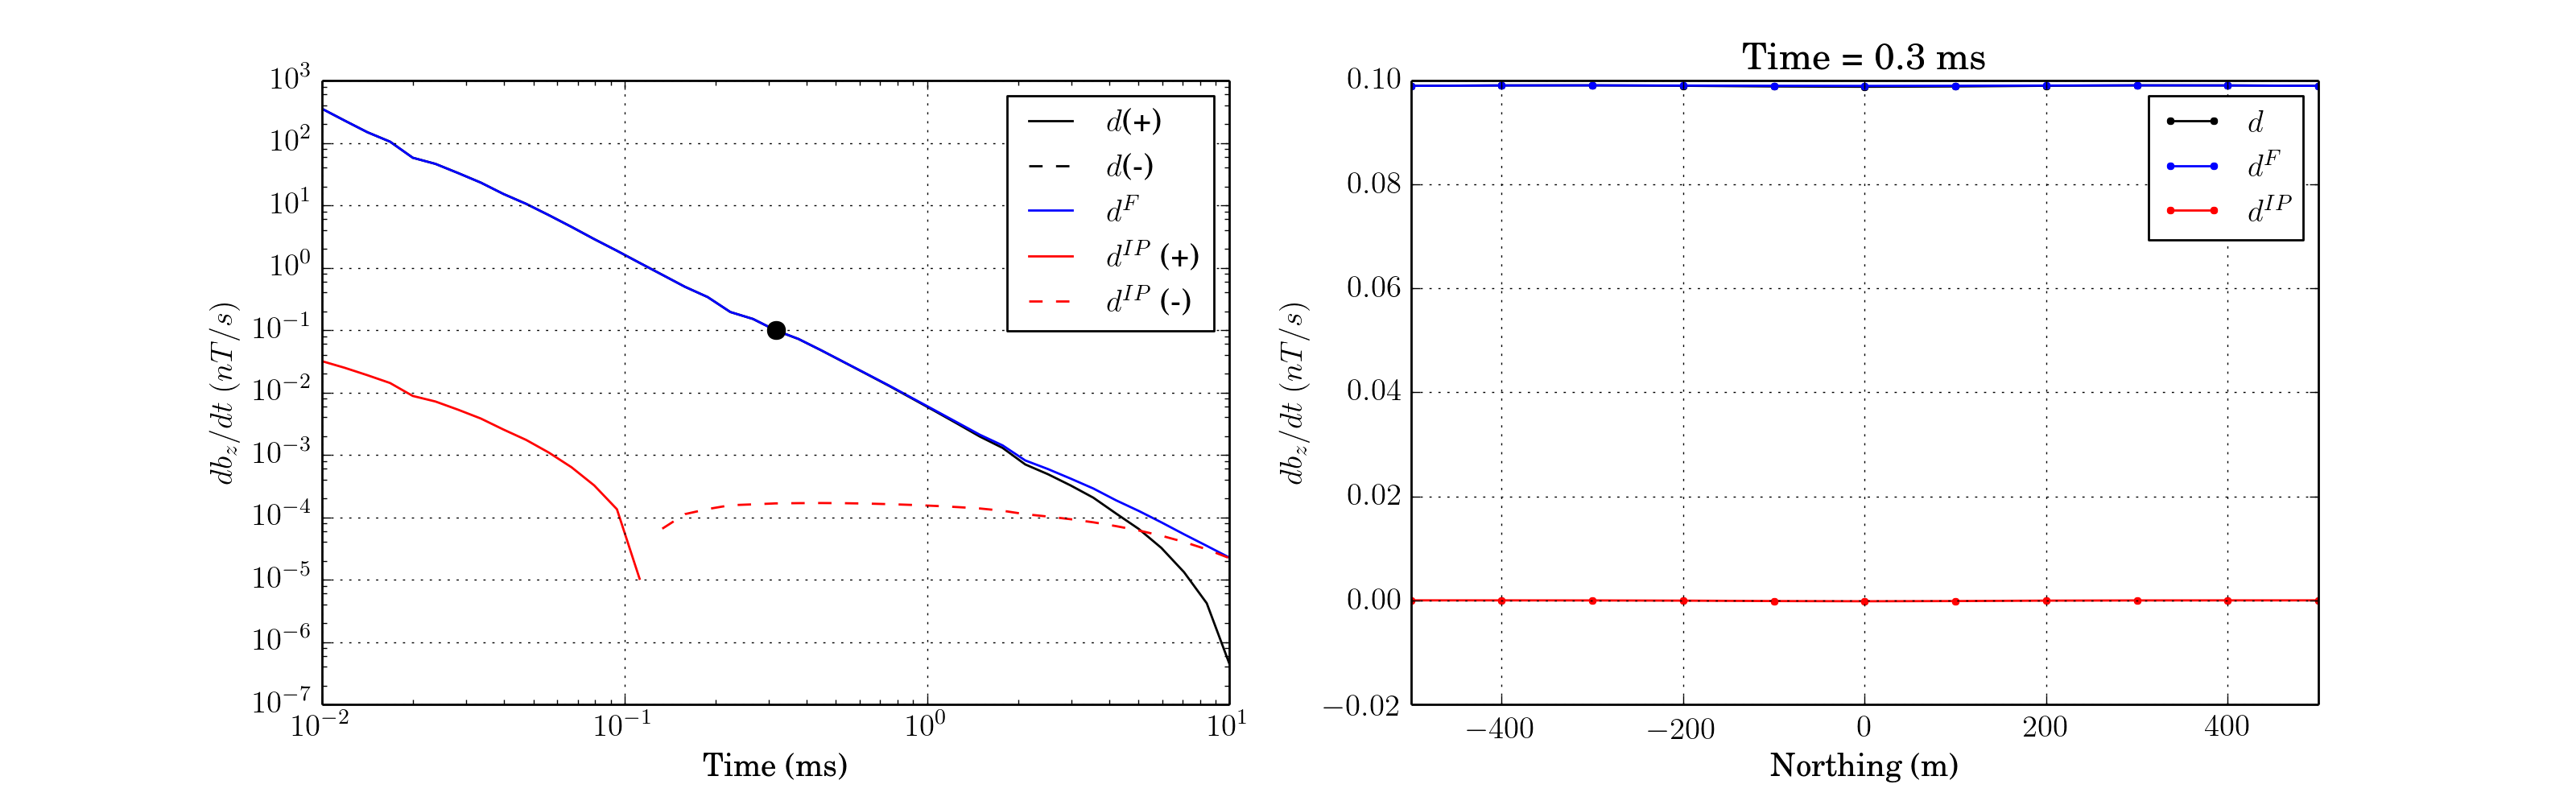
\includegraphics[height=0.2\textheight]{figures/synthetic/EMIPCase1_ch20_profile.png} \\ (a)
  \\
  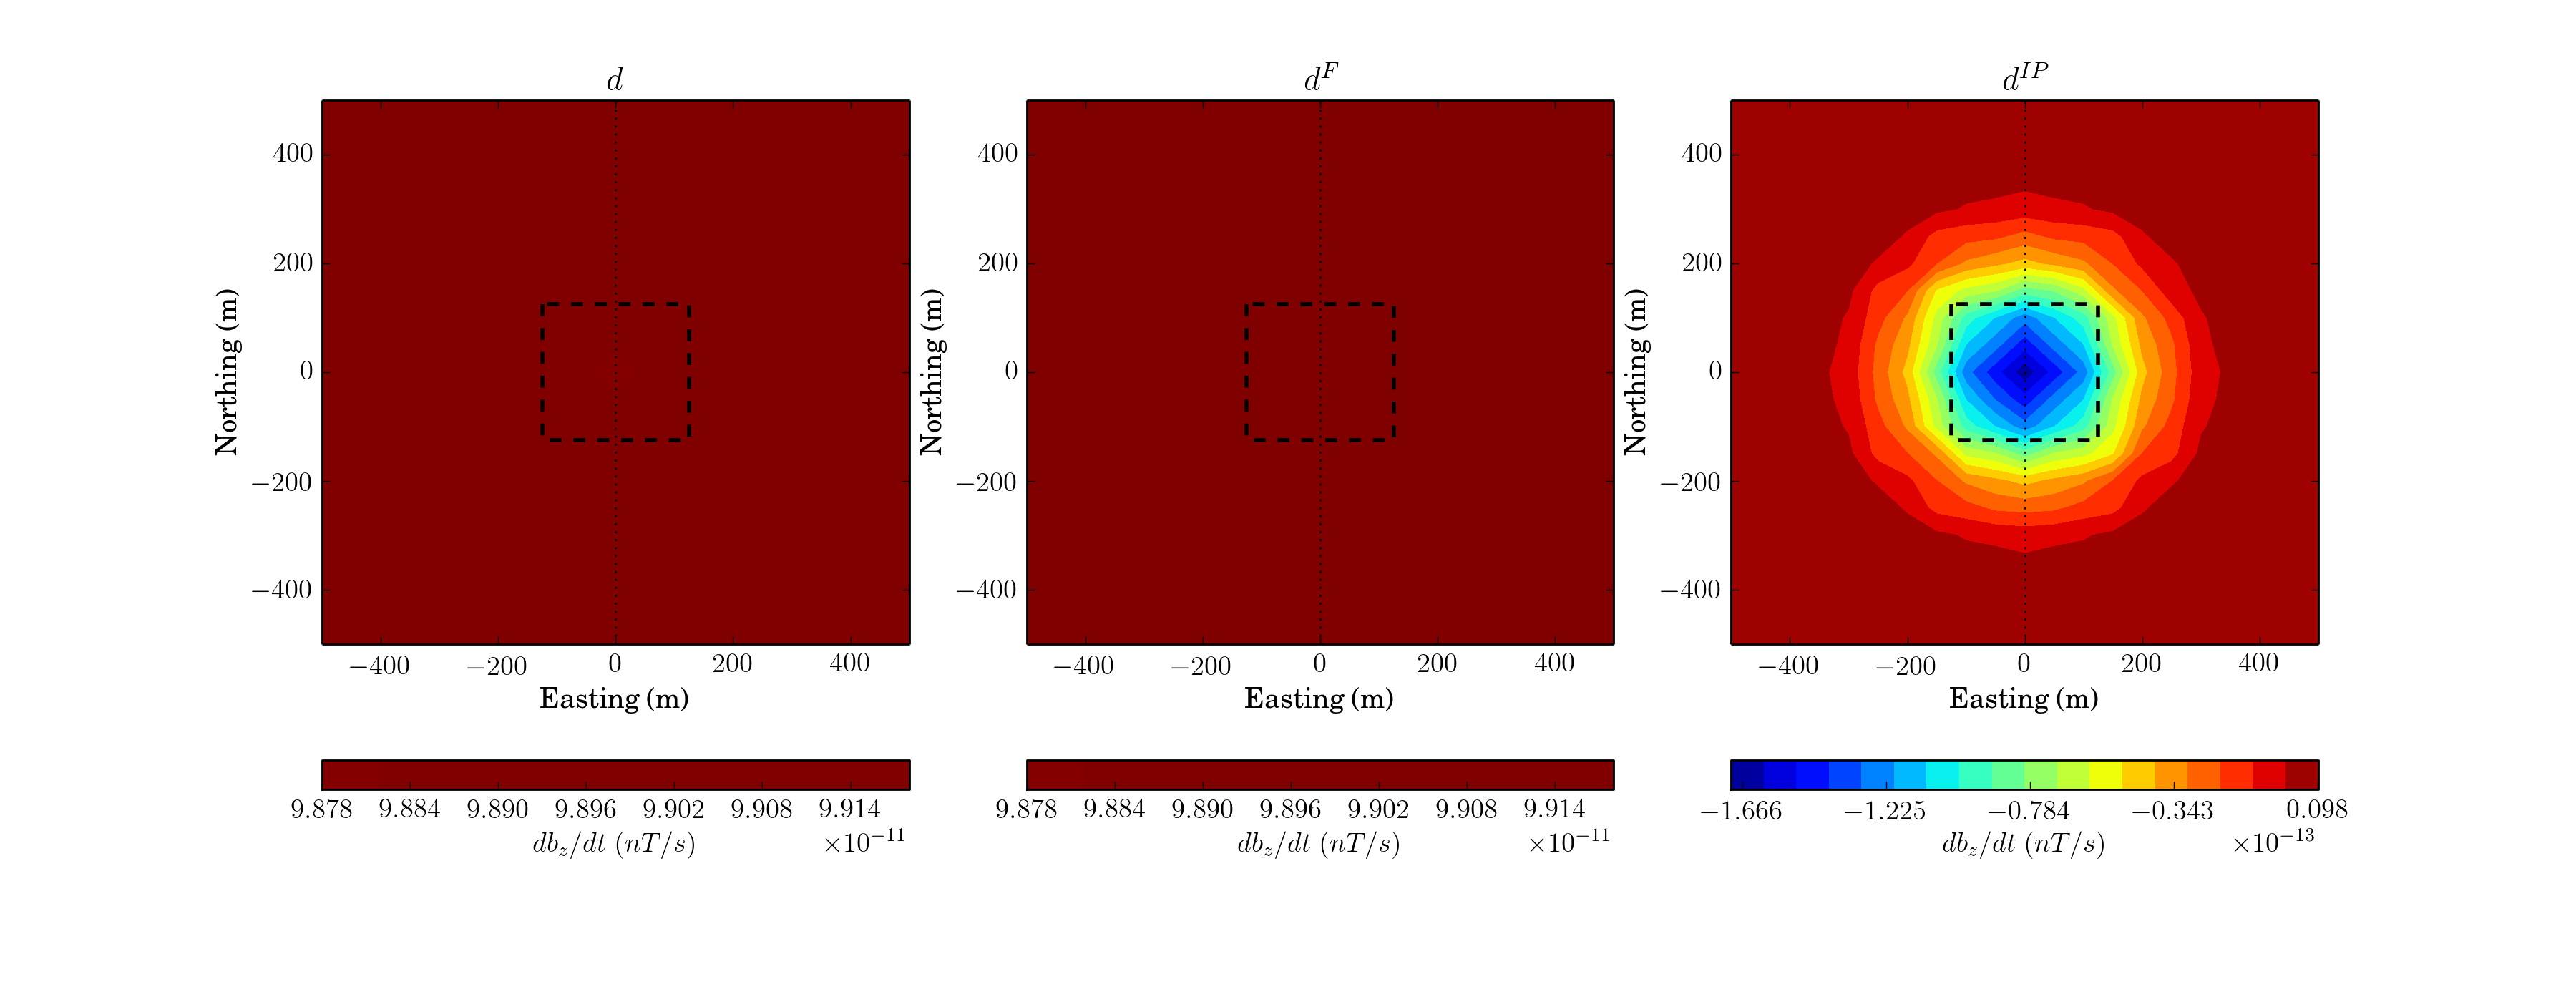
\includegraphics[height=0.25\textheight]{figures/synthetic/EMIPCase1_ch20_plan.png} \\ (b)
  \caption{Responses of $d$, $d^{F}$ and $d^{IP}$ at $t=0.37$ ms for canonical model. (a) Time decaying curves at the center sounding location (left panel) and northing profile at center line (right panel). (b) Interpolated maps of $d$ (left panel), $d^{F}$ (middle panel) and $d^{IP}$ (right panel) at all sounding locations. Black dotted line indicates the profile lines, which are shown at bottom-right panel, and black dashed line outlines IP body. Black, blue and red curves indicate $d$, $d^{F}$ and $d^{IP}$responses, respectively; solid and dotted line differentiate positive and negative values. }
  \label{F: EMIPresp1_case1}
\end{figure}
\begin{figure}[htb]
  \centering
  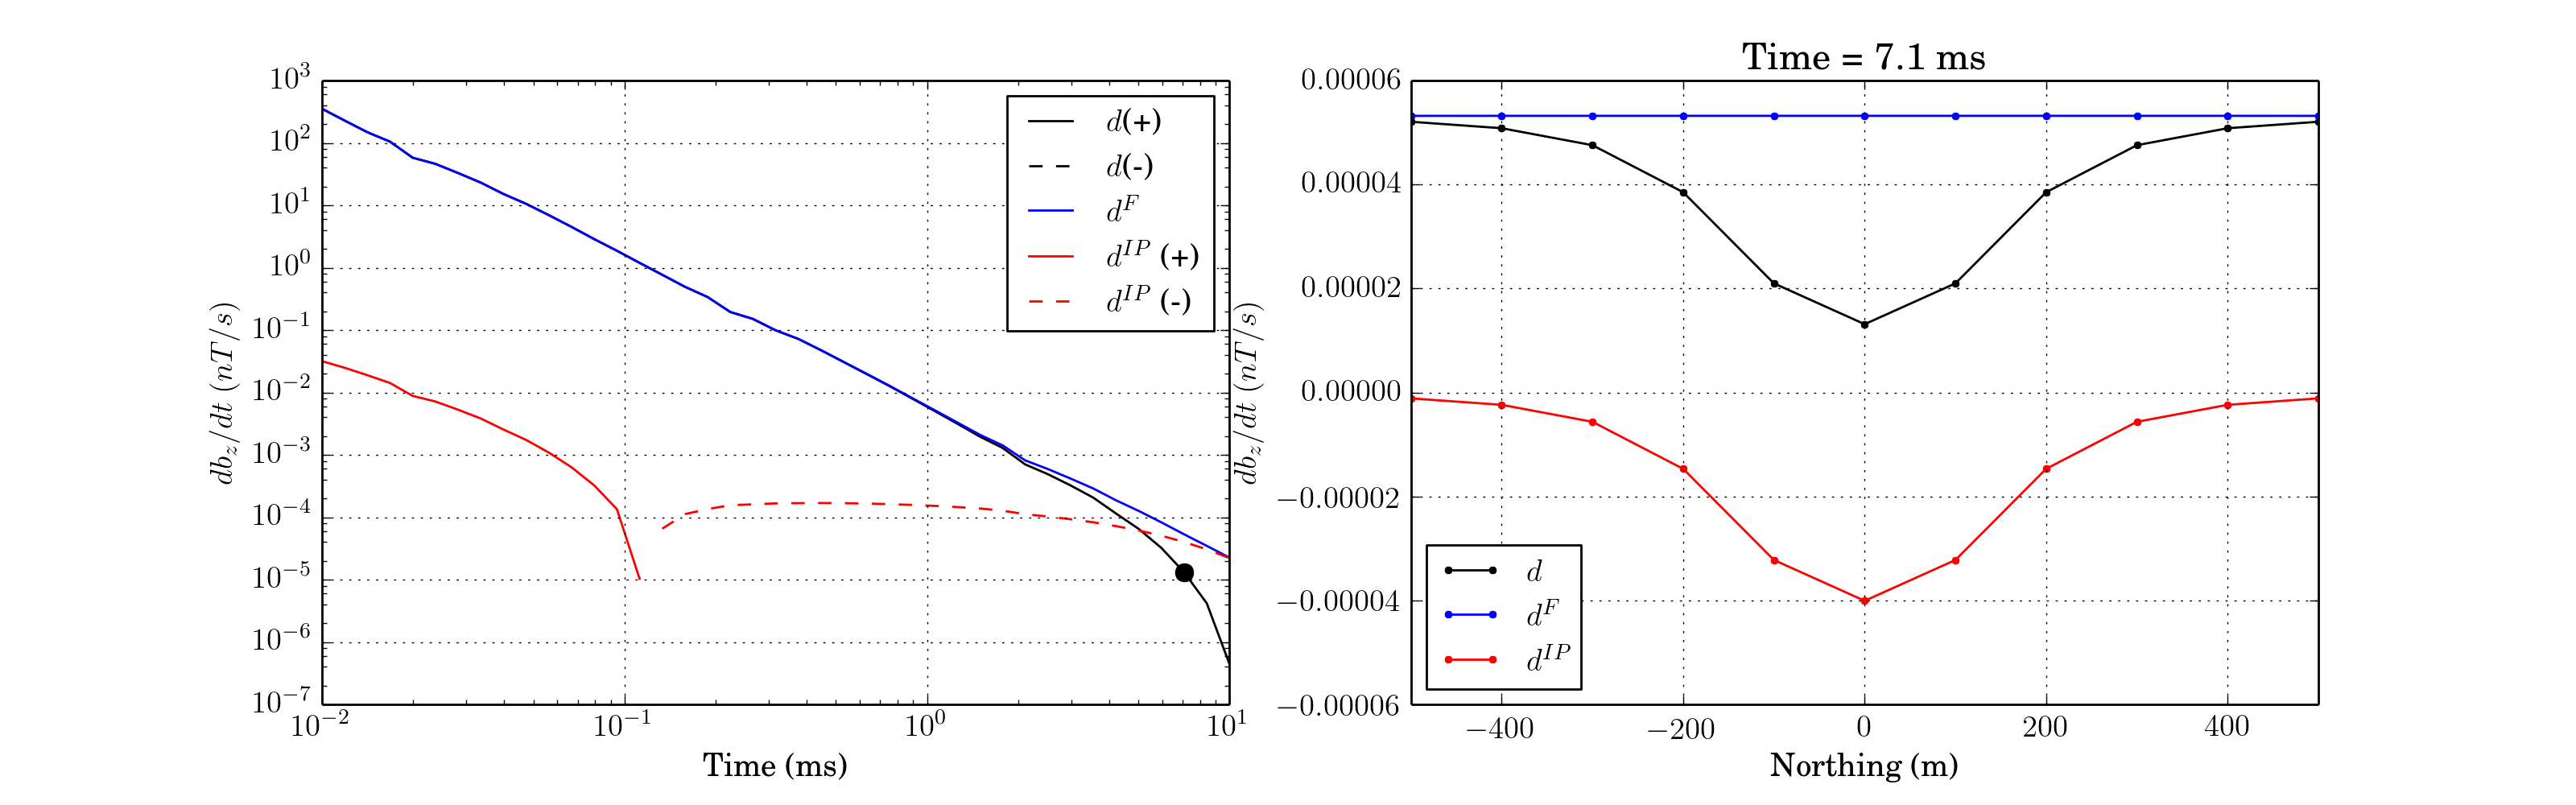
\includegraphics[height=0.2\textheight]{figures/synthetic/EMIPCase1_ch38_profile.png} \\ (a)
  \\
  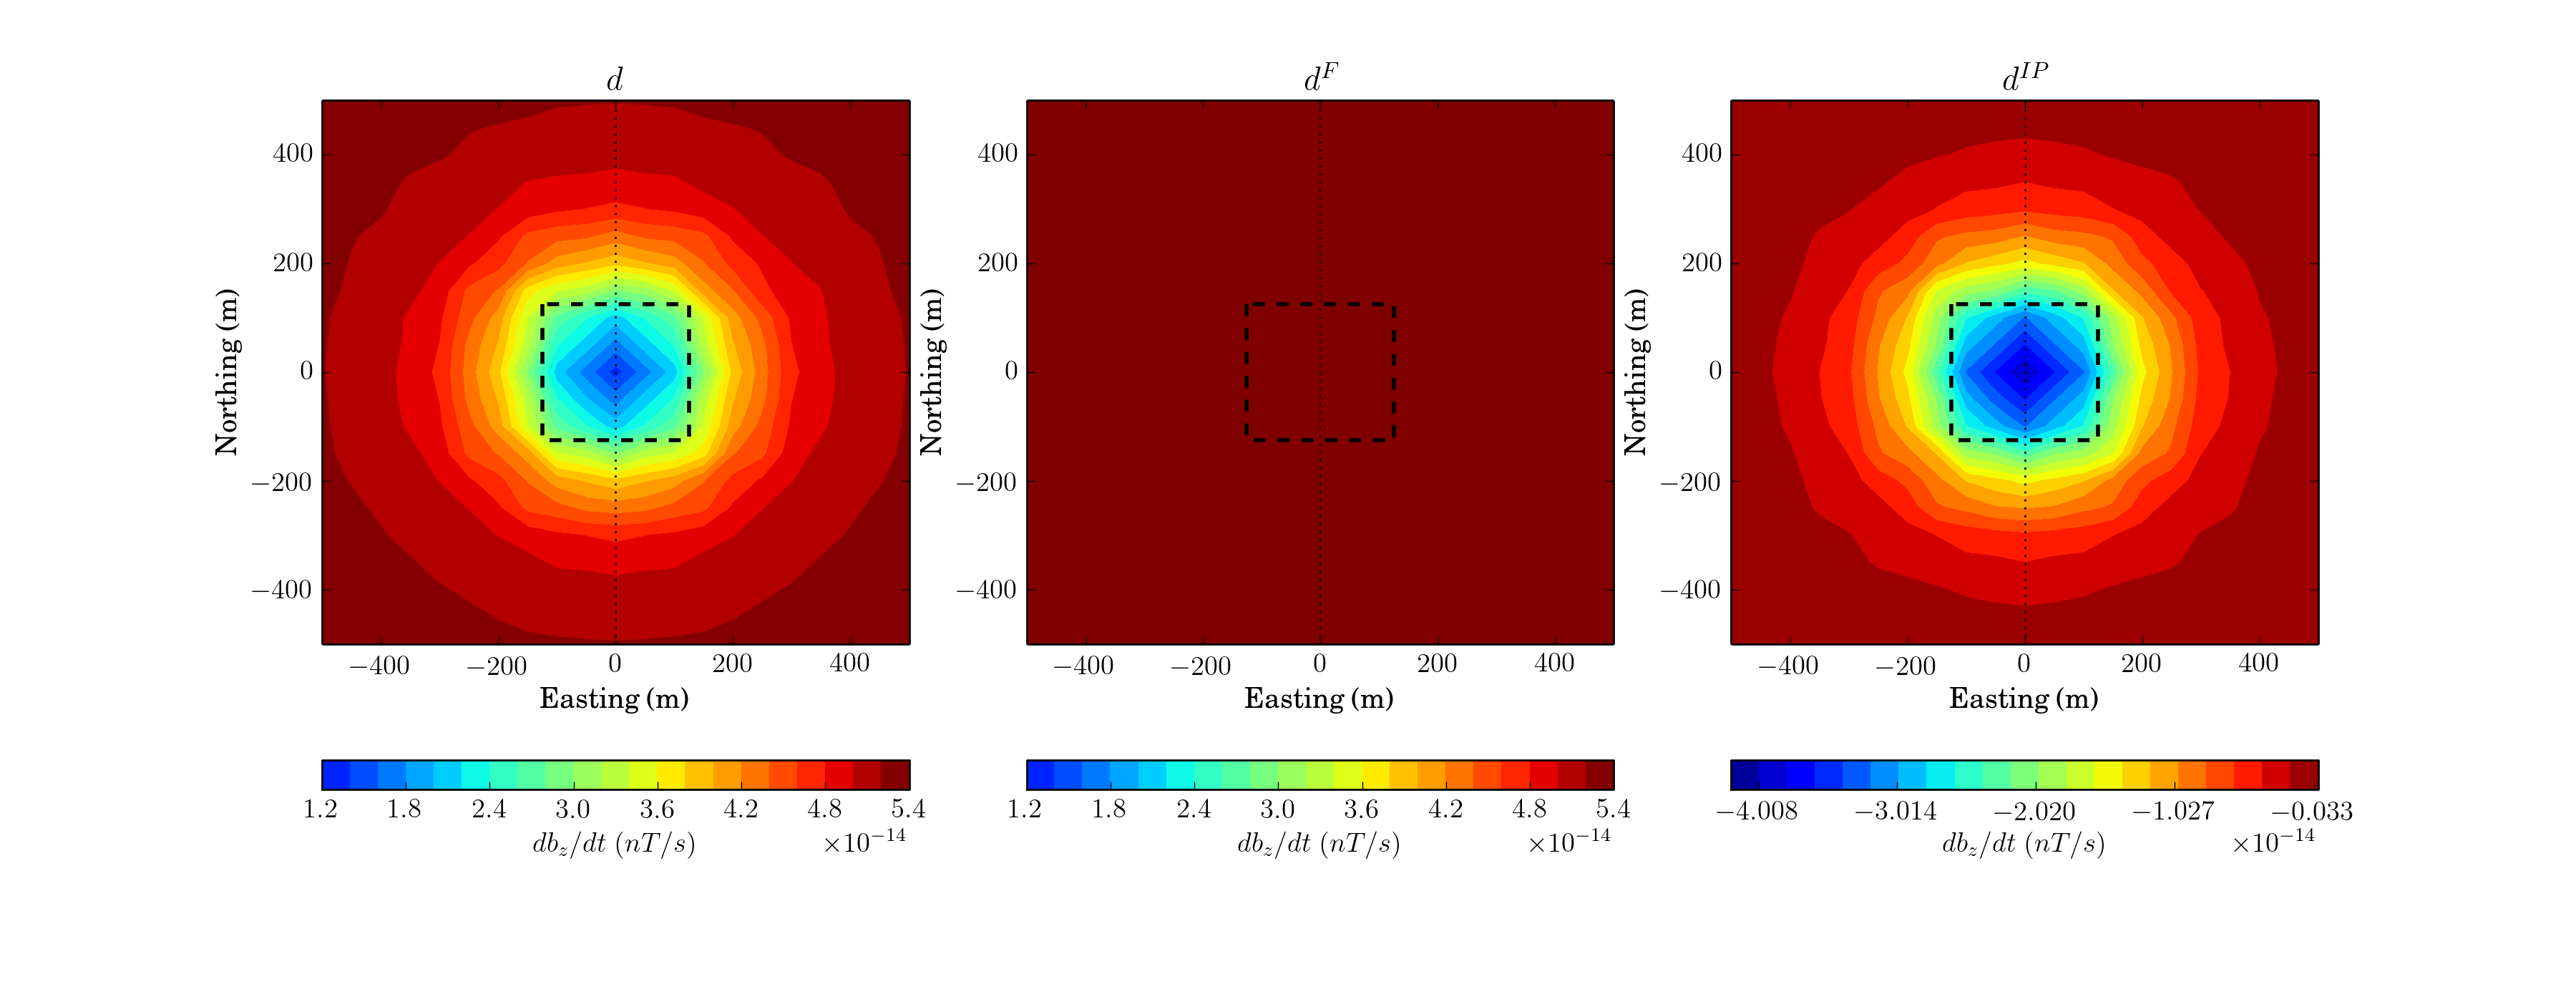
\includegraphics[height=0.25\textheight]{figures/synthetic/EMIPCase1_ch38_plan.png} \\ (b)
  \caption{Responses of $d$, $d^{F}$ and $d^{IP}$ at $t=4.7$ ms for canonical model. (a) Time decaying curves at the center sounding location (left panel) and northing profile at center line (right panel). (b) Interpolated maps of $d$ (left panel), $d^{F}$ (middle panel) and $d^{IP}$ (right panel) at all sounding locations.}
  \label{F: EMIPresp2_case1}
\end{figure}

\begin{figure}[htb]
  \centering
  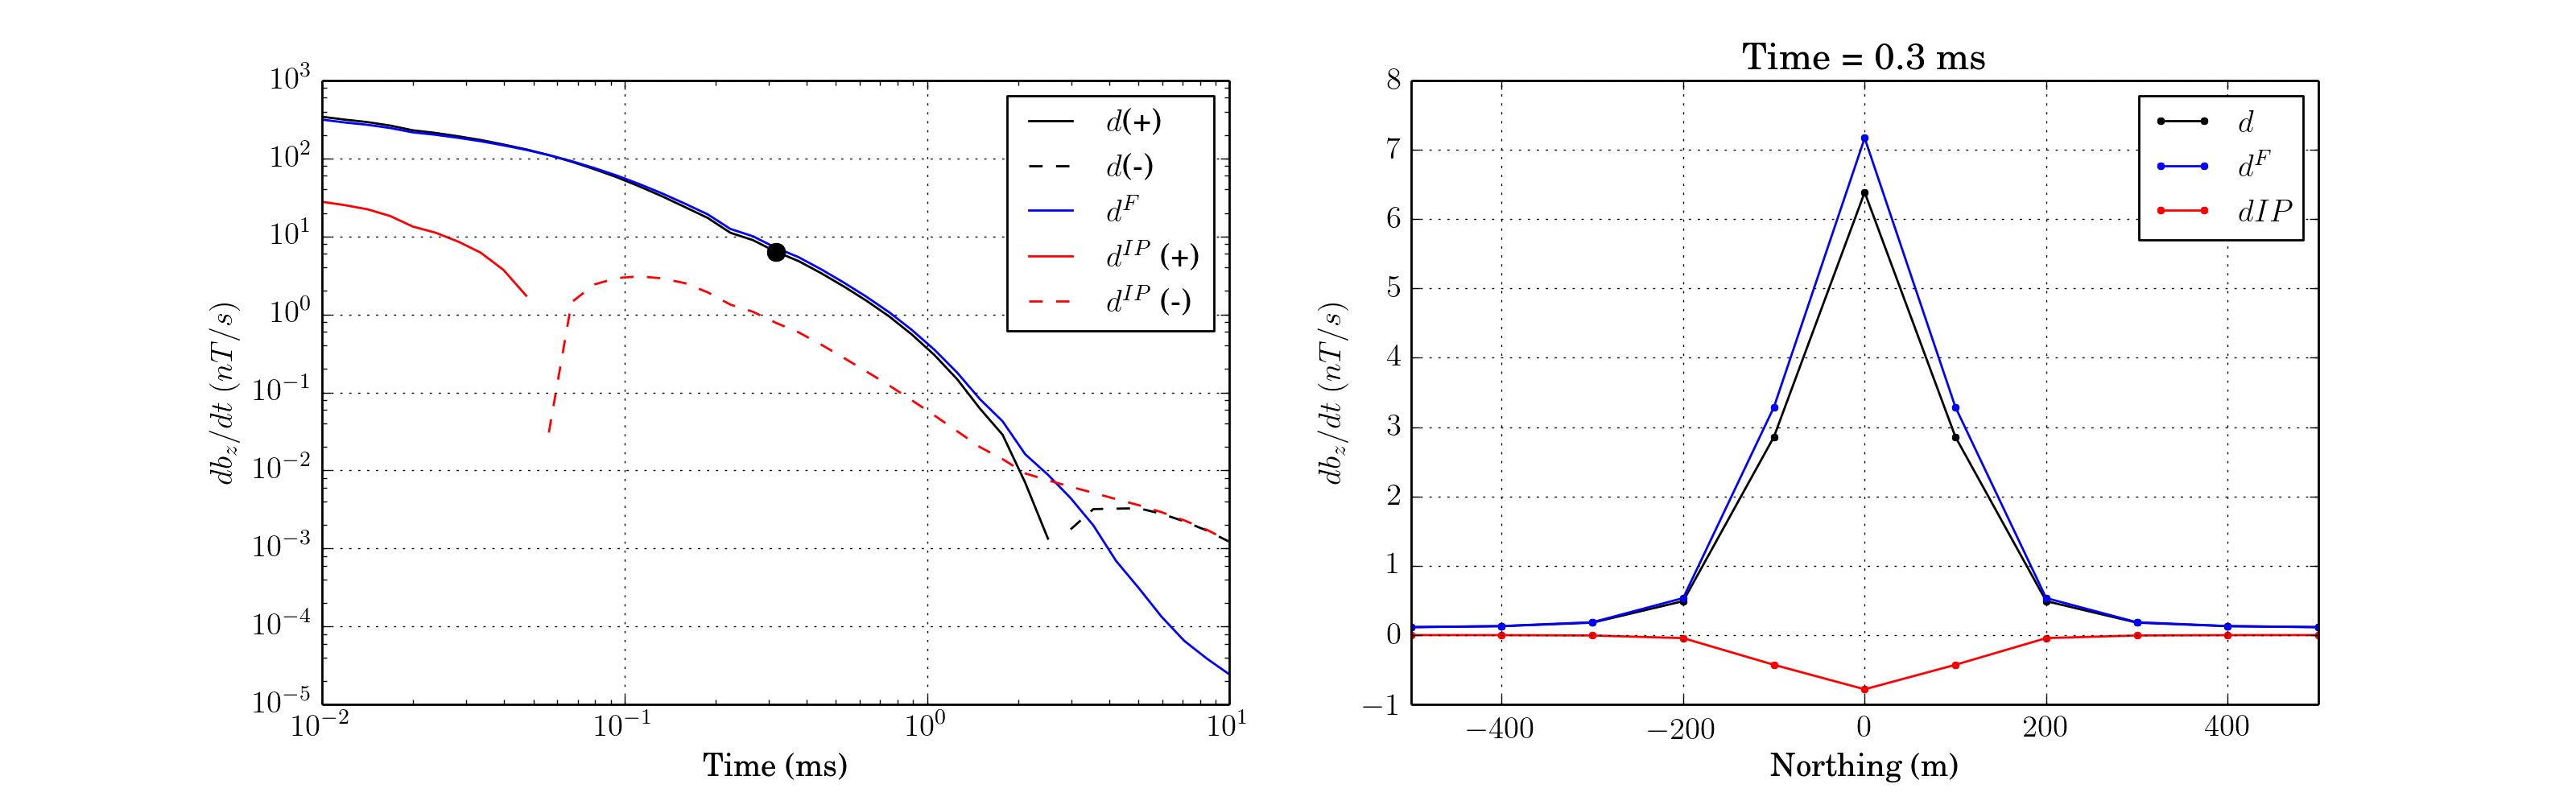
\includegraphics[height=0.2\textheight]{figures/synthetic/EMIPCase2_ch20_profile.png} \\ (a)
  \\
  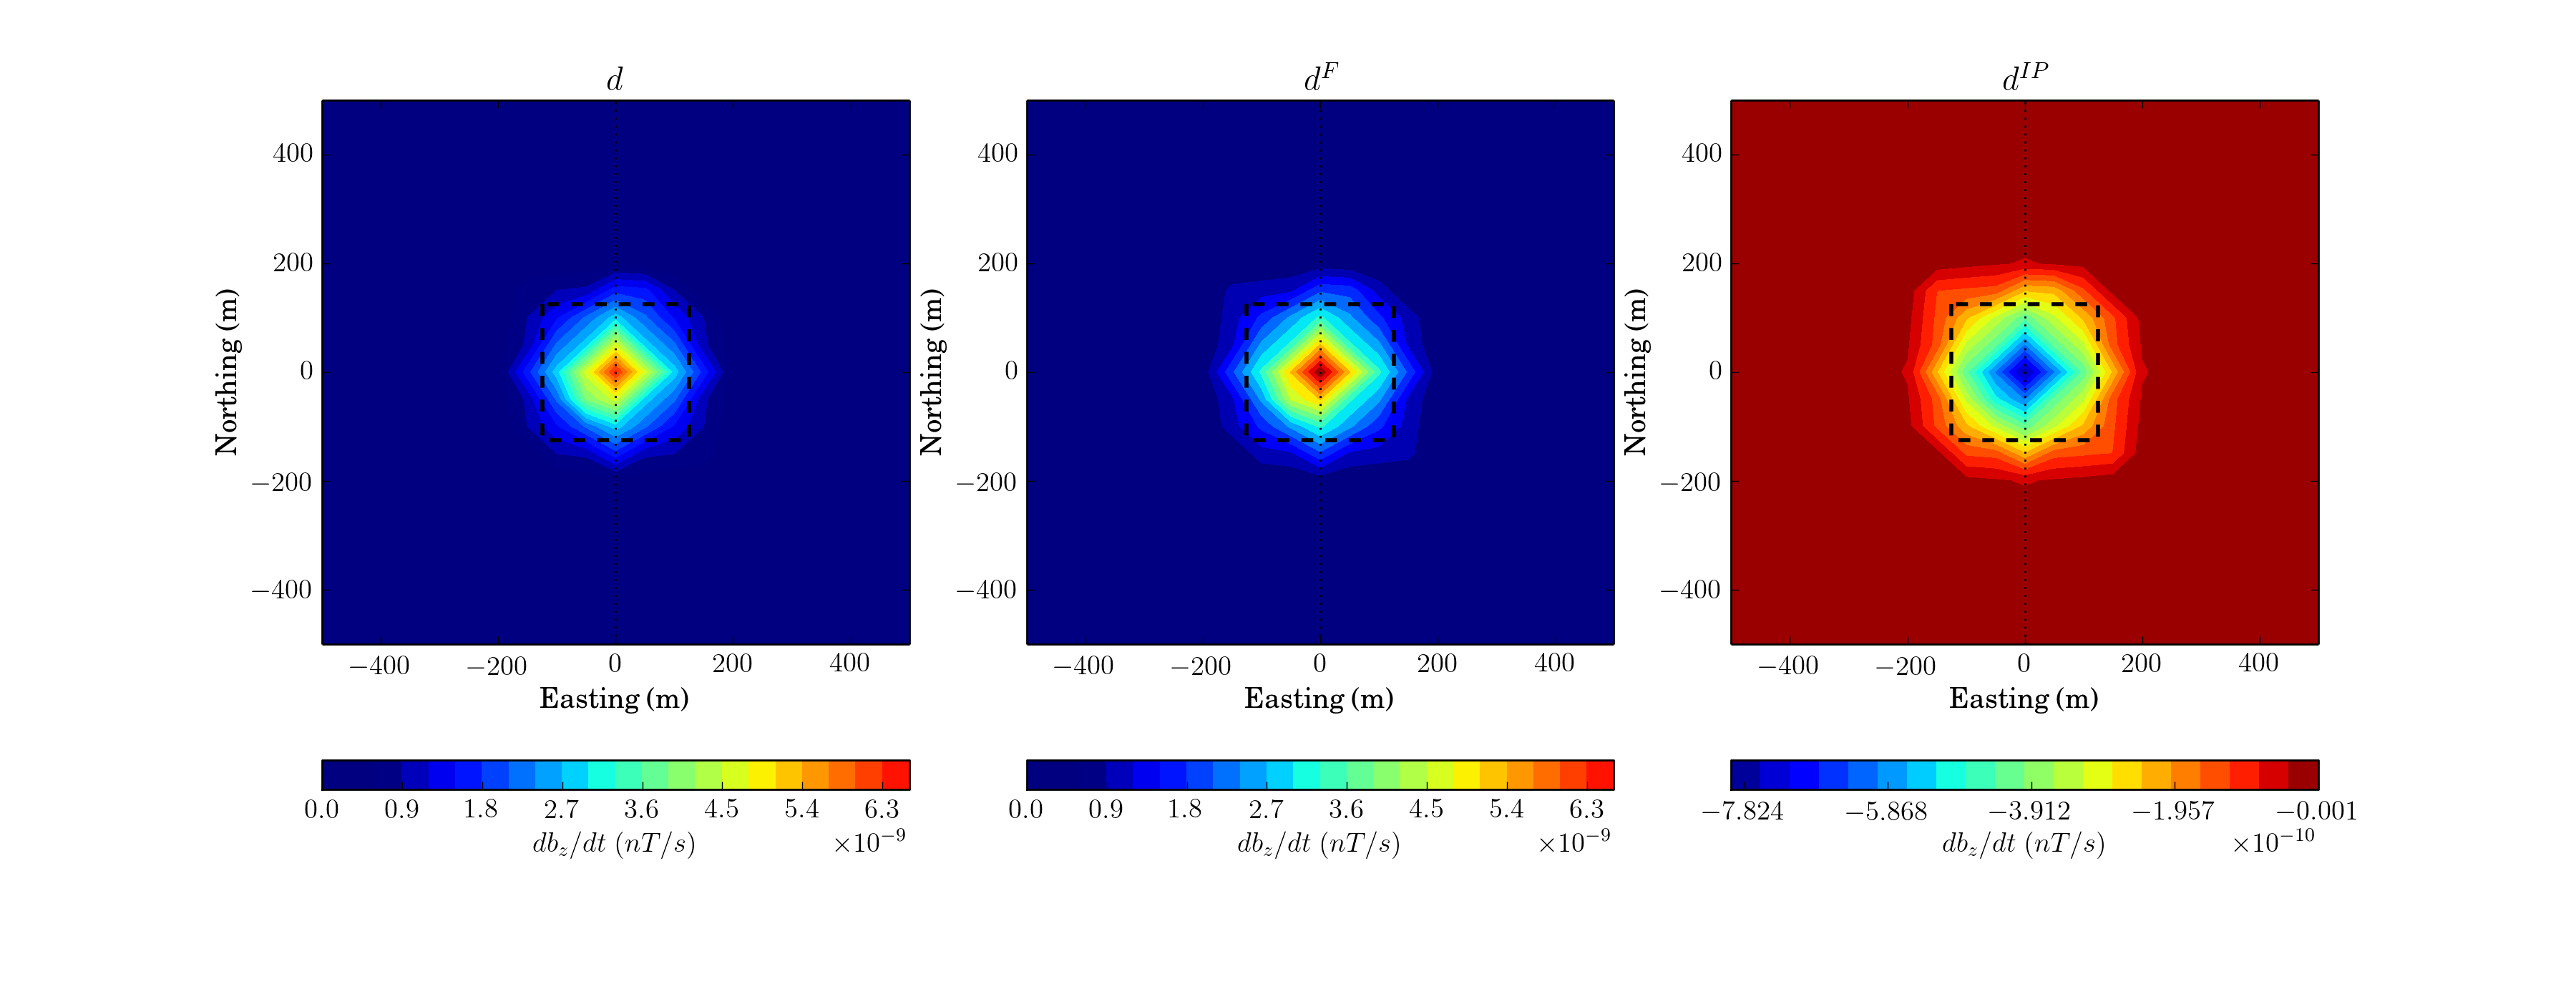
\includegraphics[height=0.25\textheight]{figures/synthetic/EMIPCase2_ch20_plan.png} \\ (b)
  \caption{Responses of $d$, $d^{F}$ and $d^{IP}$ at $t=0.37$ ms for conductive model. (a) Time decaying curves at the center sounding location (left panel) and northing profile at center line (right panel). (b) Interpolated maps of $d$ (left panel), $d^{F}$ (middle panel) and $d^{IP}$ (right panel) at all sounding locations. }
  \label{F: EMIPresp1_case2}
\end{figure}
\begin{figure}[htb]
  \centering
  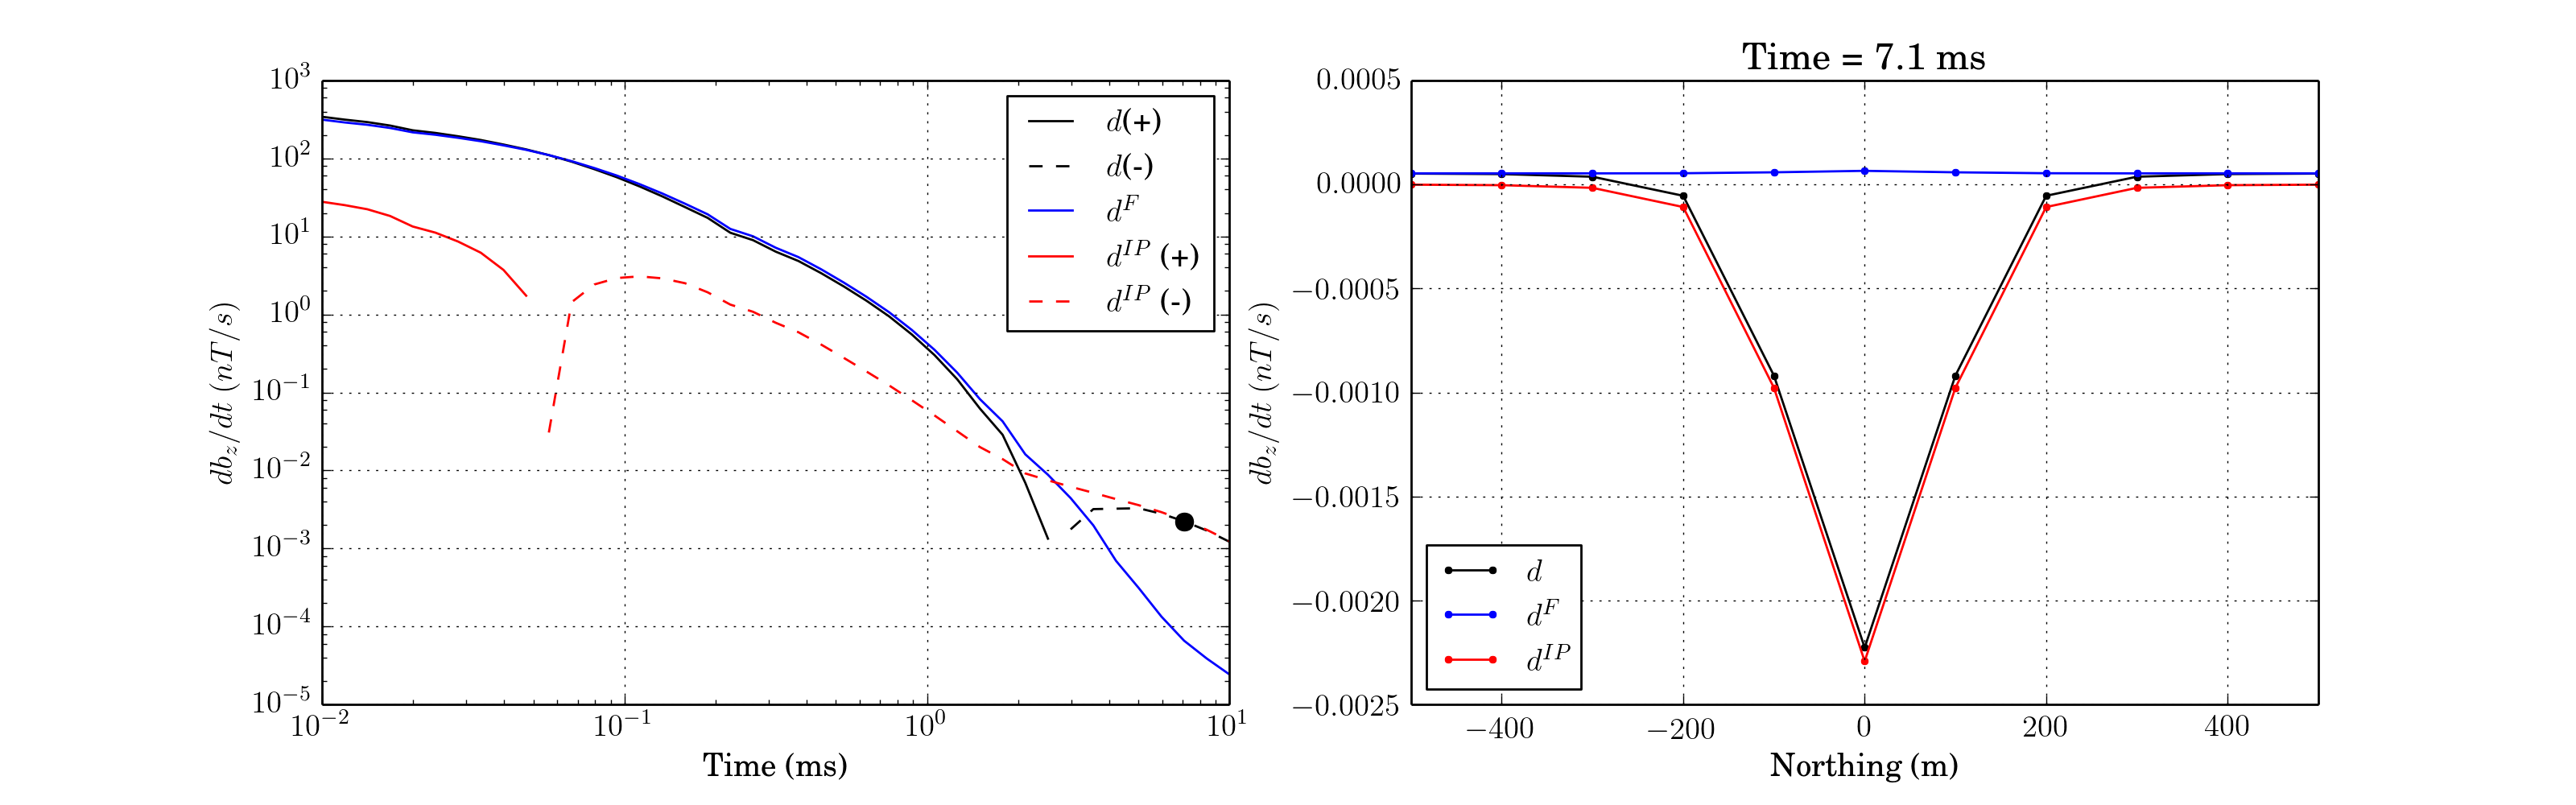
\includegraphics[height=0.2\textheight]{figures/synthetic/EMIPCase2_ch38_profile.png} \\ (a)
  \\
  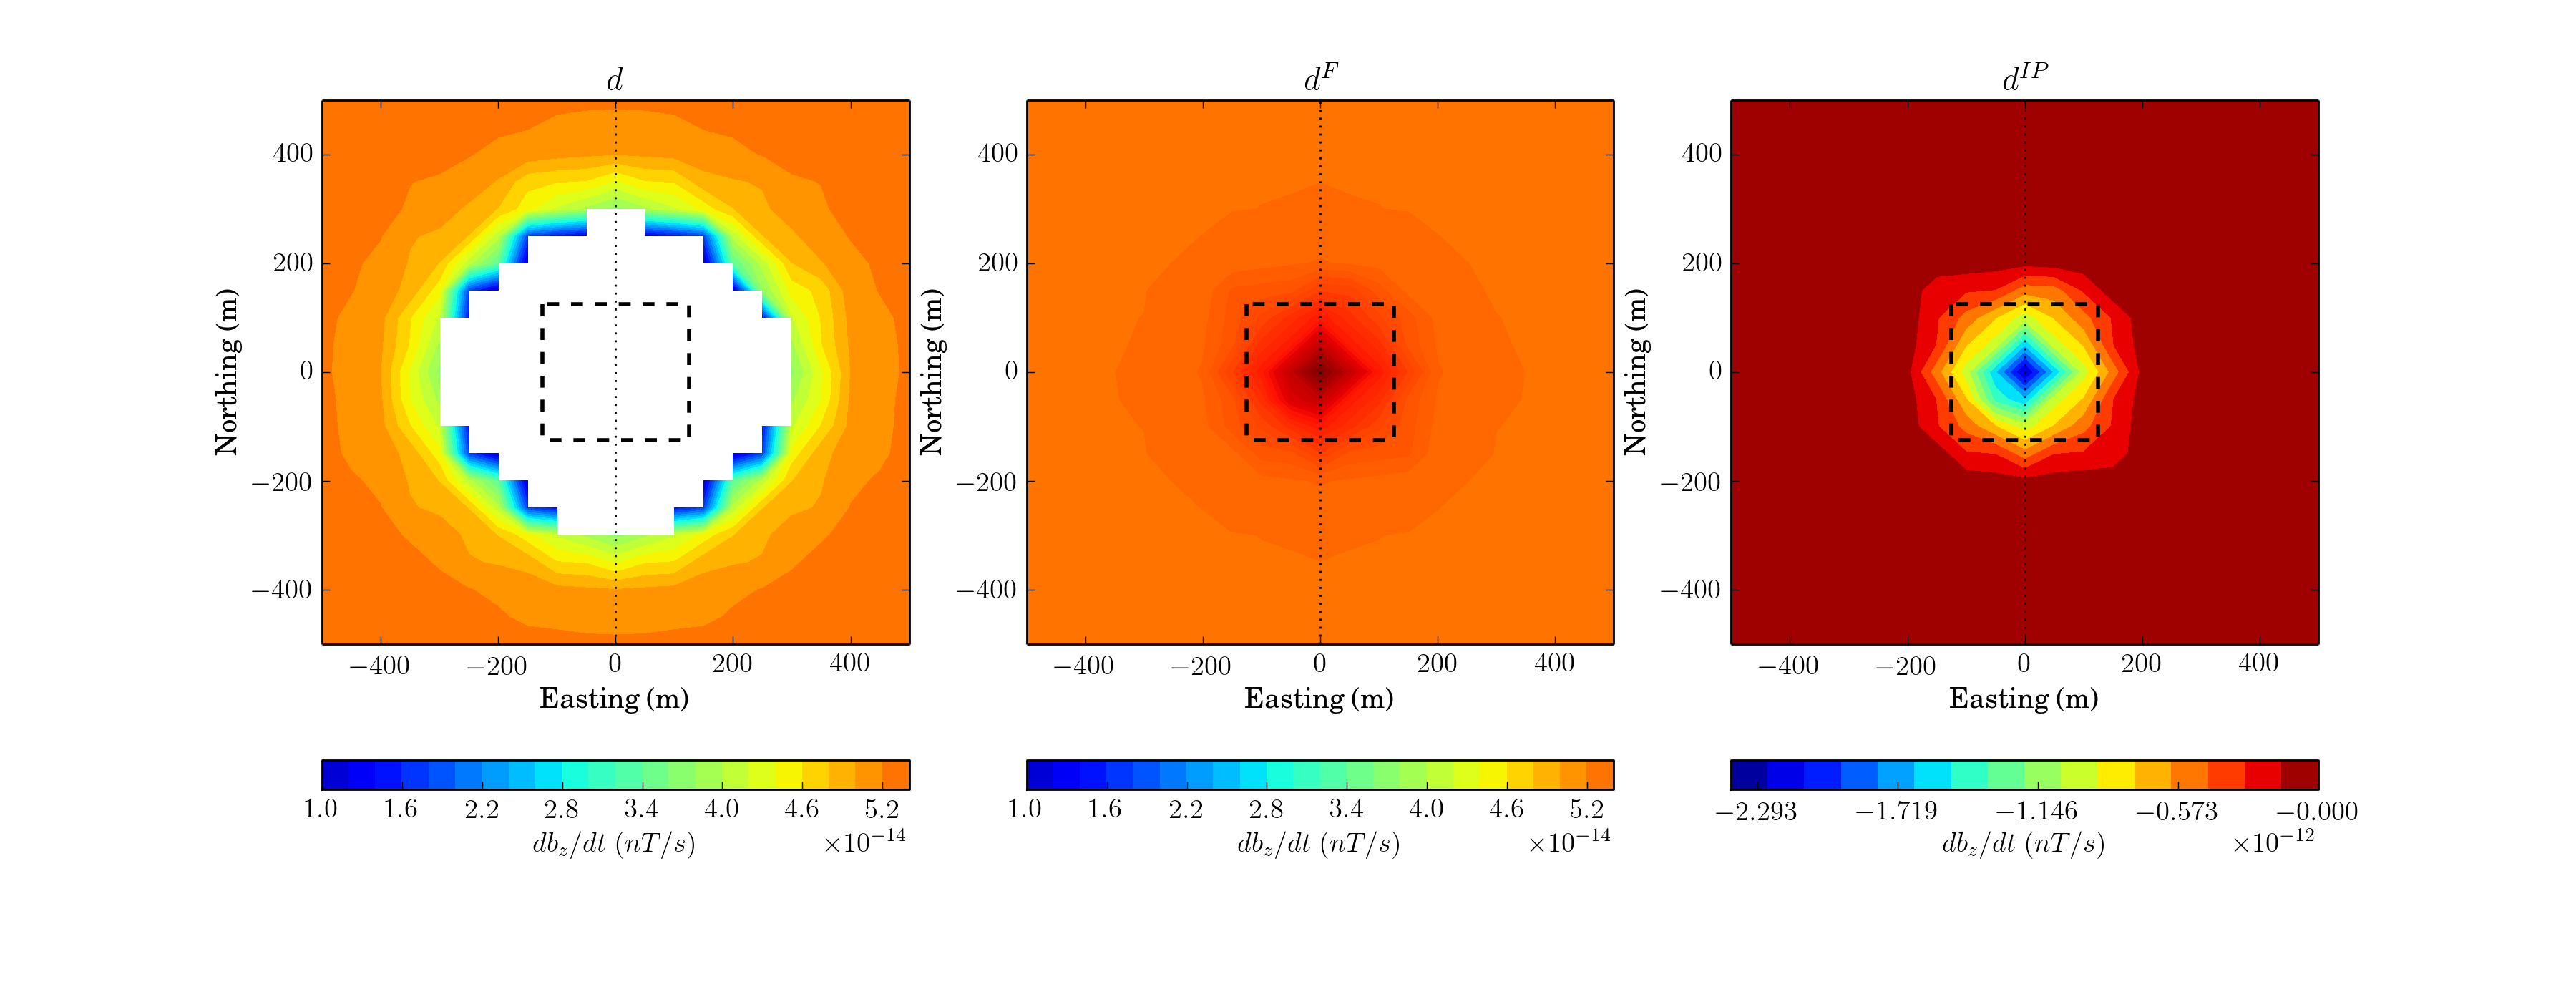
\includegraphics[height=0.25\textheight]{figures/synthetic/EMIPCase2_ch38_plan.png} \\ (b)
  \caption{Responses of $d$, $d^{F}$ and $d^{IP}$ at $t=4.7$ ms for conductive model. (a) Time decaying curves at the center sounding location (left panel) and northing profile at center line (right panel). (b) Interpolated maps of $d$ (left panel), $d^{F}$ (middle panel) and $d^{IP}$ (right panel) at all sounding locations. }
  \label{F: EMIPresp2_case2}
\end{figure}
\begin{figure}[htb]
  \centering
  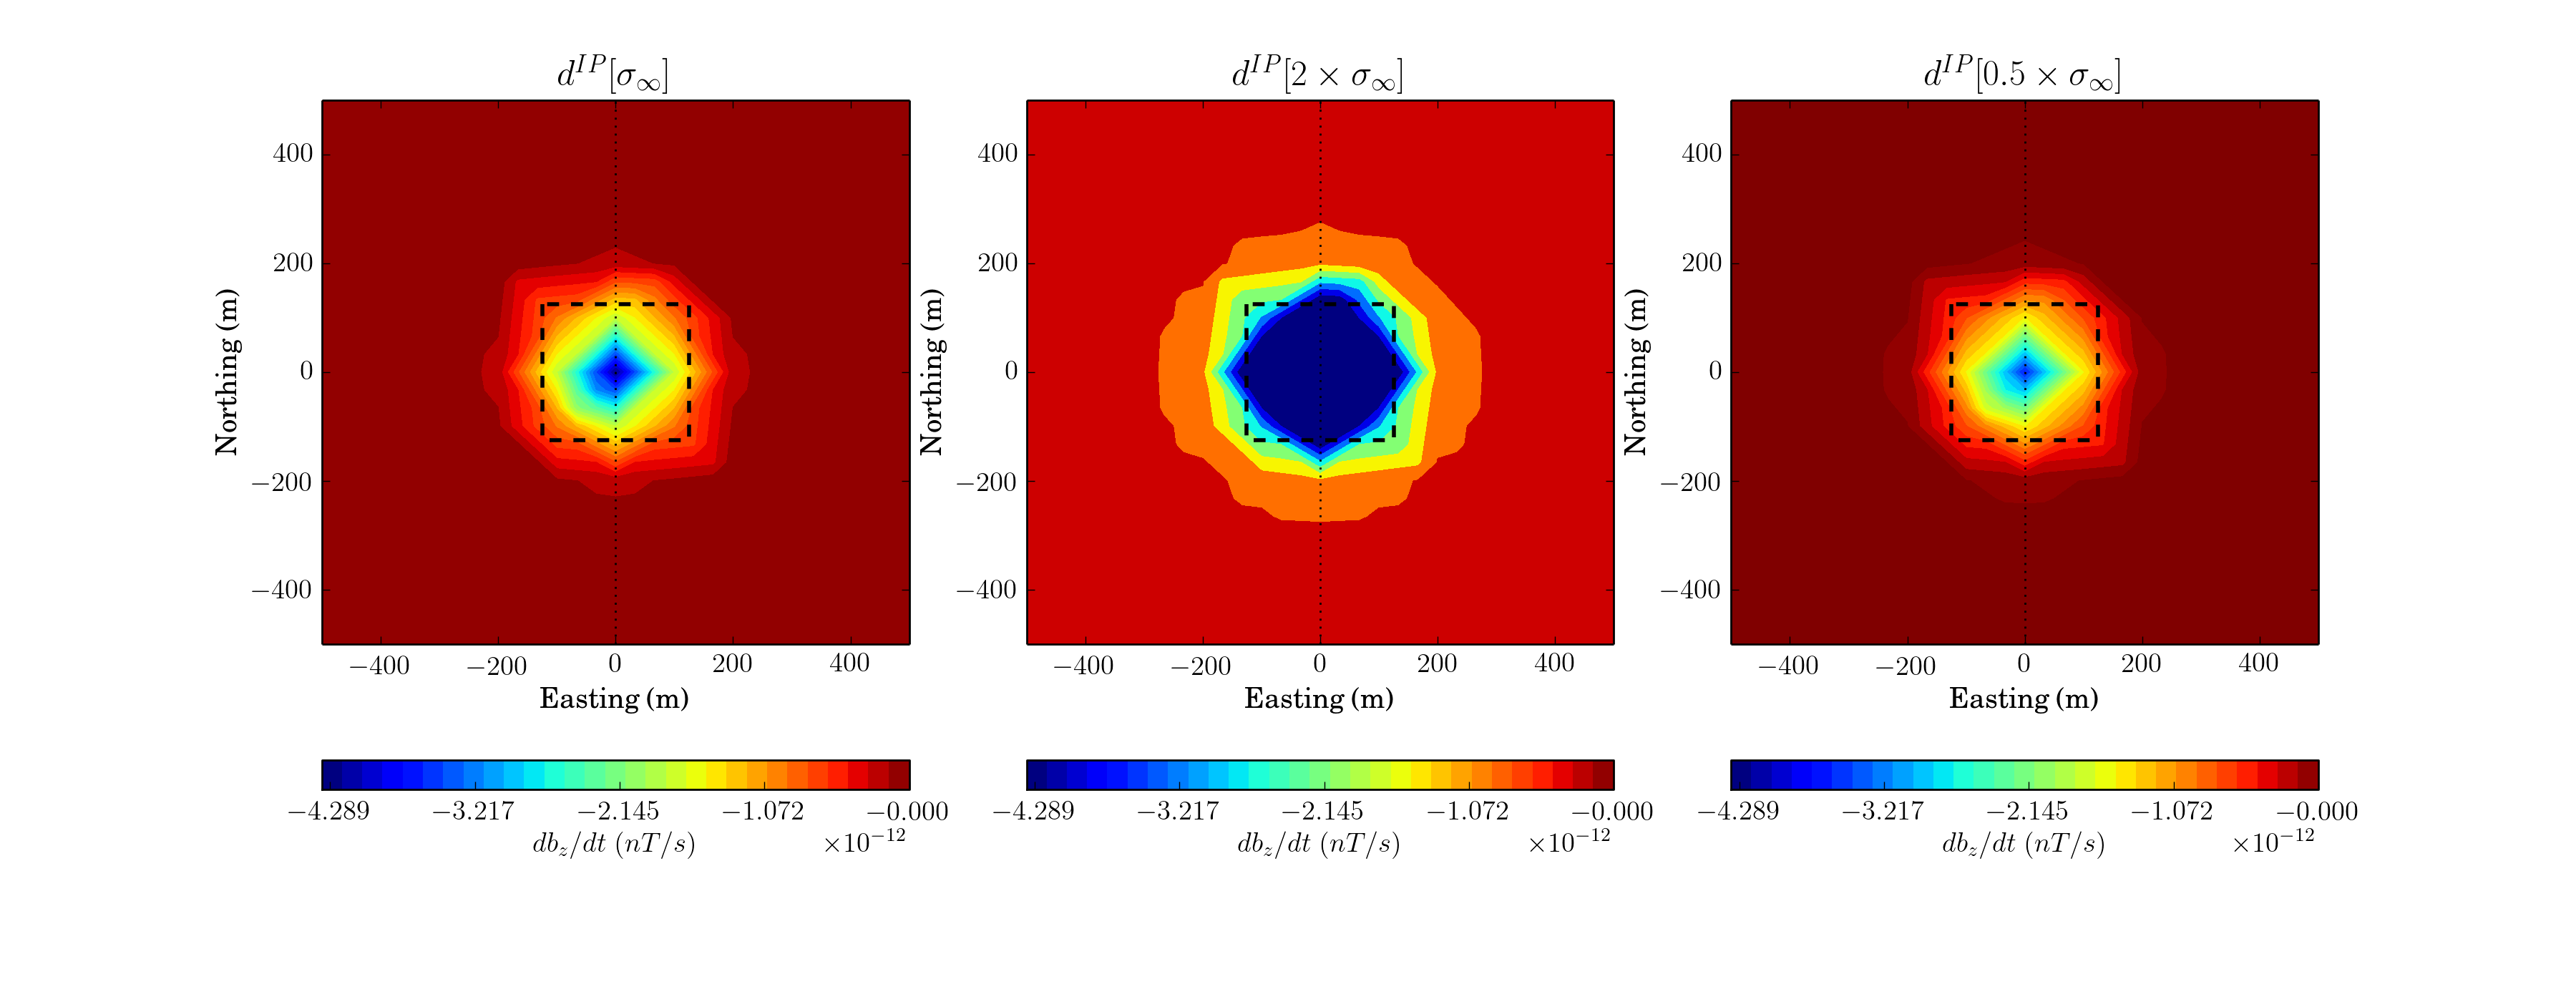
\includegraphics[height=0.25\textheight]{figures/synthetic/EMIPCase2_ch35_plan_reg.png} \\
  (a) \\
  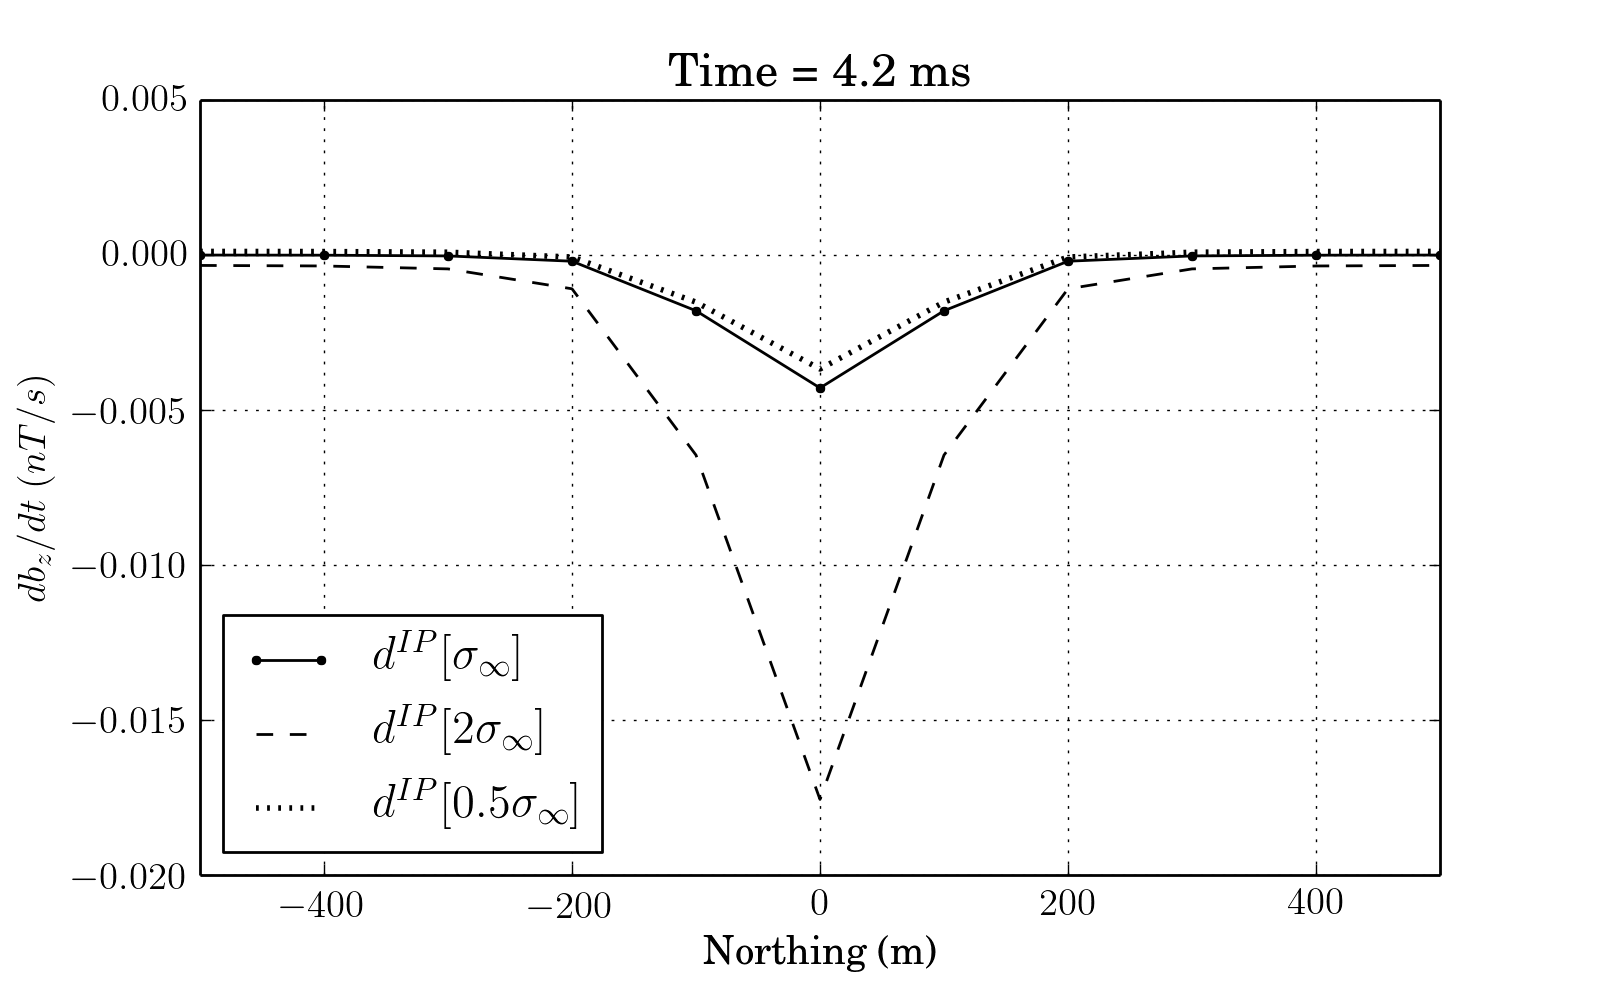
\includegraphics[height=0.25\textheight]{figures/synthetic/EMIPCase2_ch35_profile_reg.png} \\
  (b)
  \caption{$d^{IP}$ responses with correct and incorrect background conductivity models from all sounding locations (a) and the center South-North line (b) at $t = $ 2.5 ms. To compute $d^{IP}$ responses correct background conductivity model ($\sigma_{\infty}$; left panel), and 2 times of correct model (2$\sigma_{\infty}$; middle) and 0.5 times of correct model (0.5$\sigma_{\infty}$; right panel) were used. }
  \label{F: Regionalresp_case2}
\end{figure}
\clearpage

\subsection{Validation of approximation in $\j^{IP}_{approx}$}
Recall that the fundamental approximation approximation that we made to derive linear relation ship between $\d^{IP}$ and $\peta$ was that we ignore inductive effect ($\frac{\partial \b^{IP}}{\partial t} \approx 0$) in $\e^{IP}$ so that we let $\e^{IP}_{approx} = -\grad\phi^{IP}$. We compute approximated $\j^{IP}$ using this $\e^{IP}_{approx}$ as shown in equation (\ref{eq: eip_approx_full}), and then compute $\b^{IP}$ or $\frac{\partial \b^{IP}}{\partial t}$ using Biot-Savart law. Therefore, we can evaluate validity of our linearization by comparing approximated current density with true one. Before we compare $\j^{IP}$ and $\j^{IP}_{approx}$, we first investigate $\j$, $\j^{F}$ and $\j^{IP}$, since this can give us some insights about $\b^{IP}$ or $\frac{\partial \b^{IP}}{\partial t}$ which we measure in practice.

Similarly, we first treat canonical model. To investigate current density, we locate Tx at (-200, 0, -175), which indicates (Easting, Northing, Depth), and provide $\j$, $\j^{F}$ and $\j^{IP}$ at ?? m depth. In Figure \ref{F: currentEMIP_case1_plan} we presented those at t=0.37 and 7 ms. At t=0.37 ms, $\j$ and $\j^{F}$ show similar magnitude and direction, whereas they have significant difference in later time channel, t=4.7 ms. Although, $\j$ show significant difference in early and late time channels, geometry of $\j^{IP}$ between those time channels does not vary significantly whereas magnitude of them are decaying in time. This is analogous results to our conceptual model for IP responses. In addition, IP body for this case acts like a dipole, which has opposite direction to $\j^{\ ref}$. Here corresponding $\j^{\ ref}$ is $\siginf\e^{F}_{max}$. We presented  $\siginf\e^{F}_{max}$ and $t^{max}$ in the left and right panels of Figure ~\ref{F: JmaxTmaxCase1_plan}, respectively. To identify time dependent characteristics of those three current densities, we put Rx at (100, 0, -175). In Figure ~\ref{F: currentEMIP_case1_decay}a, we plotted transients of $j_y$, $j_y^{F}$ and $j_y^{IP}$ in $y$-direction. In early time range ($10^{-3}$-$10^{-1}$ ms), $j_y$ and $j_y^F$ are almost same, which shows significant EM coupling. Fundamental current density increases until it reaches to the maximum then it decays. $j_y^{IP}$ emerges in $j_y$ near t = $10^0$ ms. This supports our choice of $\e^{\  ref}$ as $\e^{F}_{max}$. As shown in equation (\ref{eq: jip_three}), $\j^{IP}$ was decomposed as three terms:
\begin{eqnarray*}
    \j^{IP} = \siginf\e^{IP} + \dsig\otimes\e^F+\dsig\otimes\e^{IP} \\
            = \j^{IP}_1 + \j^{IP}_2 + \j^{IP}_3.
\end{eqnarray*}
Since we know all components shown in above equation, we can compute all three $\j^{IP}$ terms separately. In Figure \ref{F: currentEMIP_case1_decay}b, we presented transients of each current density with same Tx and Rx locations above. In early time range ($10^{-3}$-$10^{-4}$ ms), both $\j^{IP}_1$ and $\j^{IP}_2$ are significant, whereas effect of $\j^{IP}_1$ is negligible. As we go later time channels, $\j^{IP}_2$ is getting more dominant. Effect of $\j^{IP}_3$ increases as time increases, but still negligible in our time ranges.

We evaluate approximation in $\j^{IP}$ as we referred in the beginning of this section. For this, we compare $\j^{IP}$ and $\j^{IP}_{approx}$. In Figure \ref{F: currentIP_case1_plan}, we presented plan view of $\j^{IP}$ and $\j^{IP}_{approx}$ at -175 m depth. Here we provided two different time channels t=0.37 and 7 ms (Figure \ref{F: currentIP_case1_plan}a and b). In both time channels, $\j^{IP}$ and $\j^{IP}_{approx}$ show almost same magnitude and direction. We also present time decaying curves at Rx location in Figure \ref{F: currentIP_case1_decay}. Here we provide $j_y^{IP}$, $j_{y \ 1}^{IP}$ and $j_{y \ 1 \ approx}^{IP}$, since our assumption is applied in $\e^{IP}$, which is only related to $\j^{IP}_1=\siginf\e^{IP}$. In early time range ($10^{-3}$-$10^{-1}$ ms), there are signicant difference between $j_{y \ 1}^{IP}$ and $j_{y \ 1 \ approx}^{IP}$; however, $j_{y \ 1 \ approx}^{IP}$ converges to $j_{y \ 1}^{IP}$ as we go later time channels. This shows that our approximation is reasonable in certain late time channels, whereas it is not reasonable in early time channels where we have strong EM induction effect. Therefore, our linear inversion approach is applicable for certain late time channels where galvanic IP effect is dominant compared to inductive IP effect ($\grad\phi^{IP}\gg\vec{a}^{IP}$).

Now we apply same analyses of current density to conductive model and compare with canonical model. We presented plan view of $\j$, $\j^{F}$ and $\j^{IP}$ at t=0.37 and 7 ms in Figure \ref{F: currentEMIP_case2_plan}a and b, respectively. Similar to canonical model, $\j$ and $\j^F$ in earlier time channel are almost same, whereas those are different in later time channel due to IP effect. Different from canonical model, higher values of $\j$ and $\j^F$ are concentrated on the region where we have conductive IP body due to the strong EM induction effect. In addition, $\j^{IP}$ in earlier time channel (left panel of Figure ~\ref{F: currentEMIP_case2_plan}a) shows complicated directions so that our conceptual model seems not valid at this earlier time channel. However, in later time channel, we recognize that IP body acts like a dipole, which has opposite direction to $\siginf\e^{F}_{max}$ as shown in the right panel Figure \ref{F: JmaxTmaxCase2_plan}. This analogous to our conceptual model which implies applicability of our method in certain late time channels. We also presented $t^{max}$ in the right panel of Figure ~\ref{F: JmaxTmaxCase2_plan}.
Transients of $j_y$, $j^{F}_y$ and $j^{IP}_y$ were shown in Figure \ref{F: currentEMIP_case2_decay}a. Relative strength of maximum $j^{IP}_y$ to that of $j^{F}_y$, is greater in conductive model than canonical one which may be the reason why we have strong $d^{IP}$ responses for conductive model. Same decomposition of $\j^{IP}$ was applied to this case and all transients of $j^{IP}_{y \ 1}$, $j^{IP}_{y \ 2}$ and $j^{IP}_{y \ 3}$ are shown in Figure \ref{F: currentEMIP_case2_decay}b. Different from canonical model, $j^{IP}_{y \ 1}$ is dominant term in late time range ($10^{-3}$-$10^{-2}$ ms). Similarly, effect of $j^{IP}_{y \ 3}$ increases as we move on to later time channels, but still it is not significant in our time range. In addition, we evaluate approximation in $\j^{IP}$ for conductive model. Plan views of $\j^{IP}$ and $\j^{IP}_{approx}$ at t= 0.37 and 4.7 ms are shown in Figure ~\ref{F: currentIP_case2_plan}a and b, respectively. At t=0.37 ms, $\j^{IP}$ and $\j^{IP}_{approx}$ are different in terms of both magnitude and direction. However, in later time channel at t=4.7 ms, they show almost same magnitude and direction. We present time decaying curves of $j_y^{IP}$, $j_{y \ 1}^{IP}$ and $j_{y \ 1 \ approx}^{IP}$ in Figure \ref{F: currentIP_case2_decay}. Similarly, $j_{y \ 1 \ approx}^{IP}$ converges to $j_{y \ 1}^{IP}$, and we recognize that $\j^{IP}_1$ is the dominant term of $\j^{IP}$ for conductive case.

To summarize, in early time channel when we have significant EM induction effect, our assumption, which ignores inductive IP term in $\e^{IP}$ is not valid. However, in certain late time channels, this assumption is reasonable so that we can linearize $d^{IP}$ responses. By comparing canonical and conductive models, we recognize that conductive model can have much more EM induction effect, which makes significant complication in $\j^{IP}$ at early time channels. However, this complication disappears in certain late time channels, thus we can apply same linearization approach even for this case. Similarly, we investigated that our conceptual model can be applicable in certain later time channels. In addition, we recognize that $\j^{IP}_1$ and $\j^{IP}_2$ are the dominant term for canonical and conductive models, respectively. Effect of $\j^{IP}_3$ increases as time increases, but it was not significant in our experiments.

\begin{figure}[htb]
  \centering
  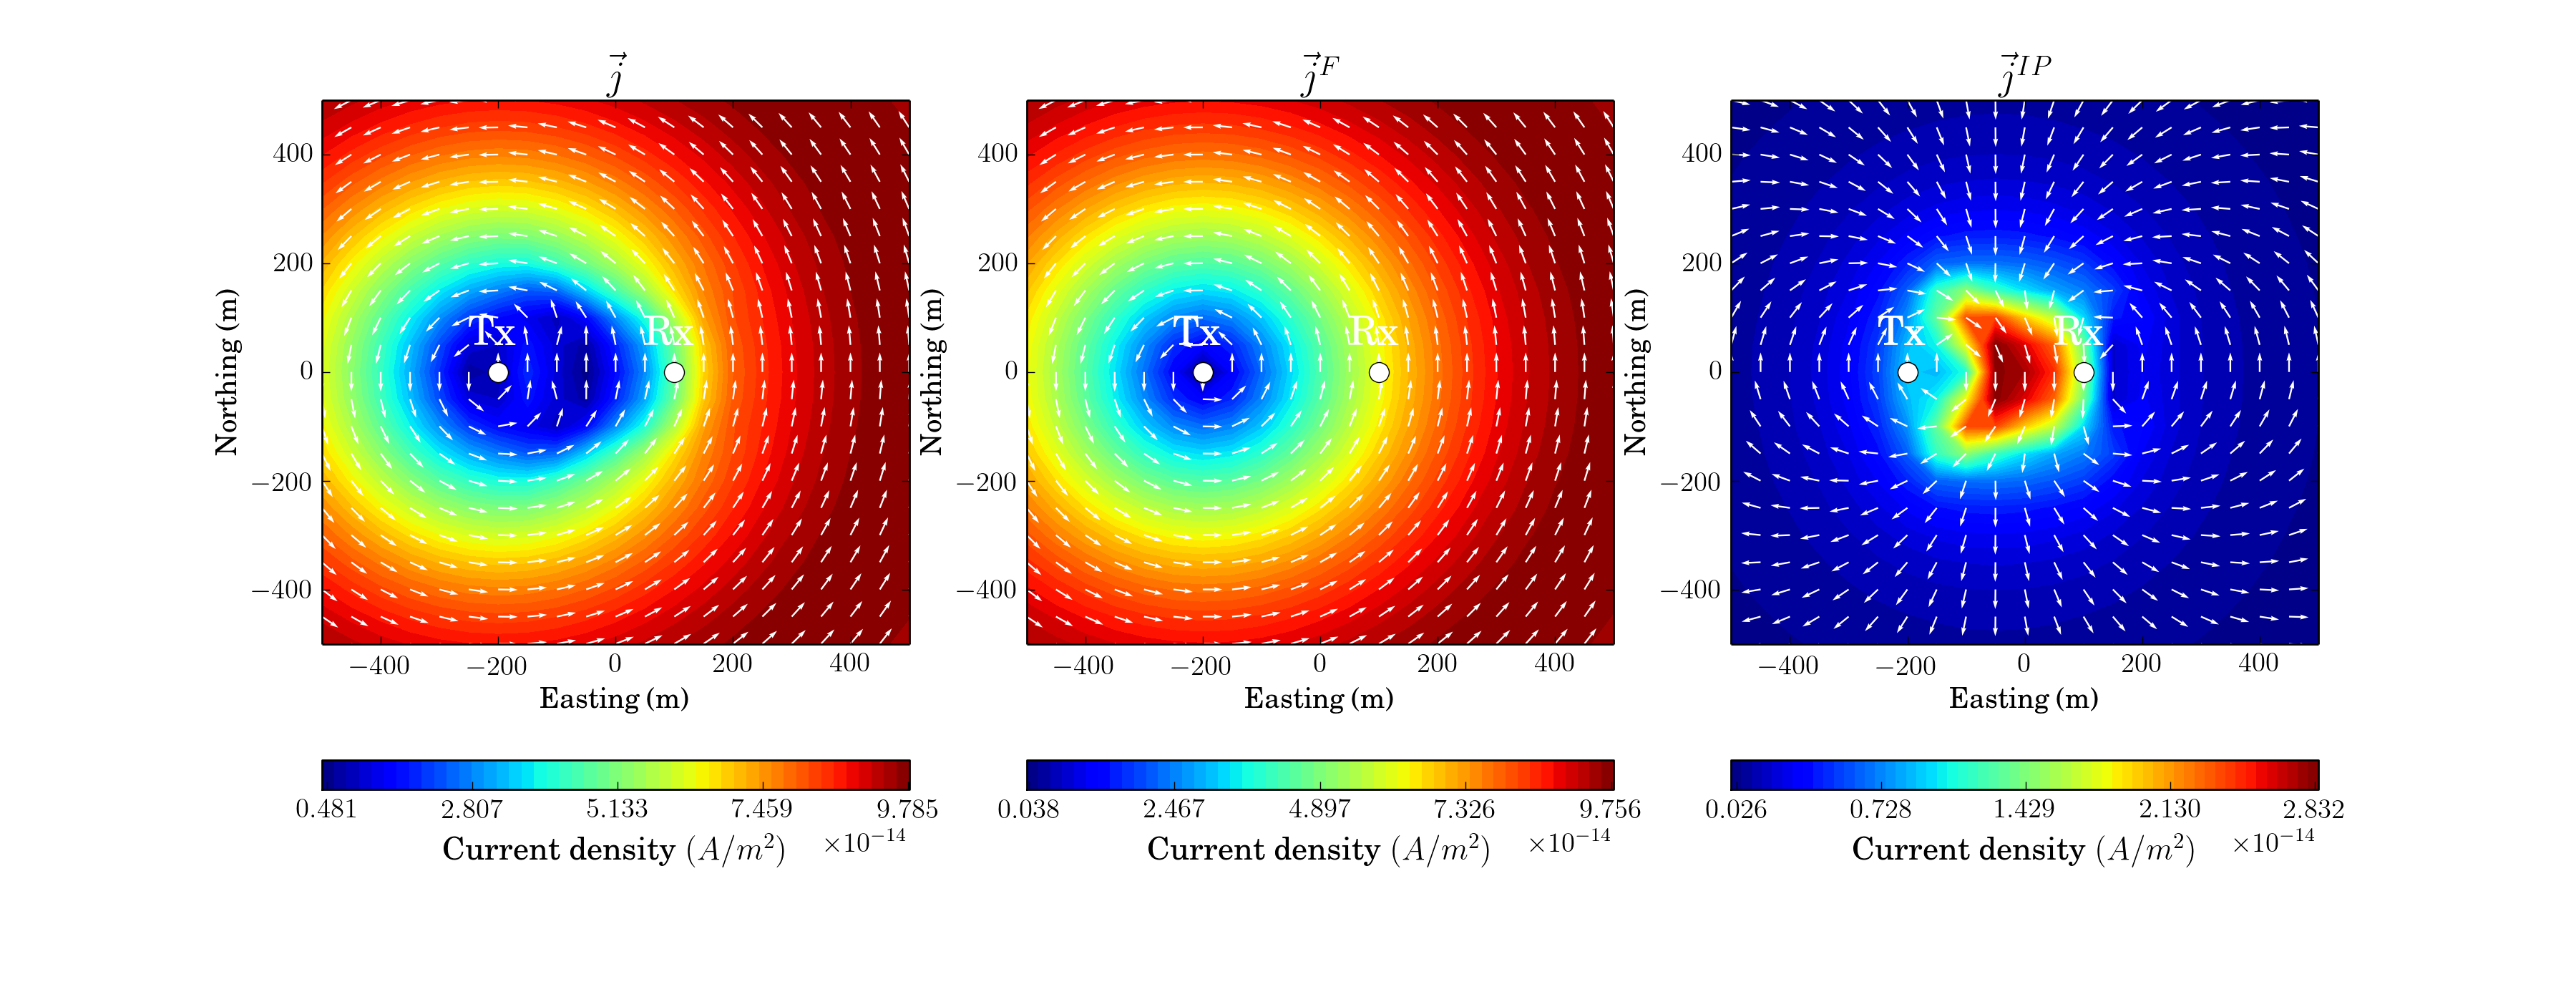
\includegraphics[height=0.25\textheight]{figures/synthetic/CurrentEMIP_case1_ch20.png} \\
  (a) \\
  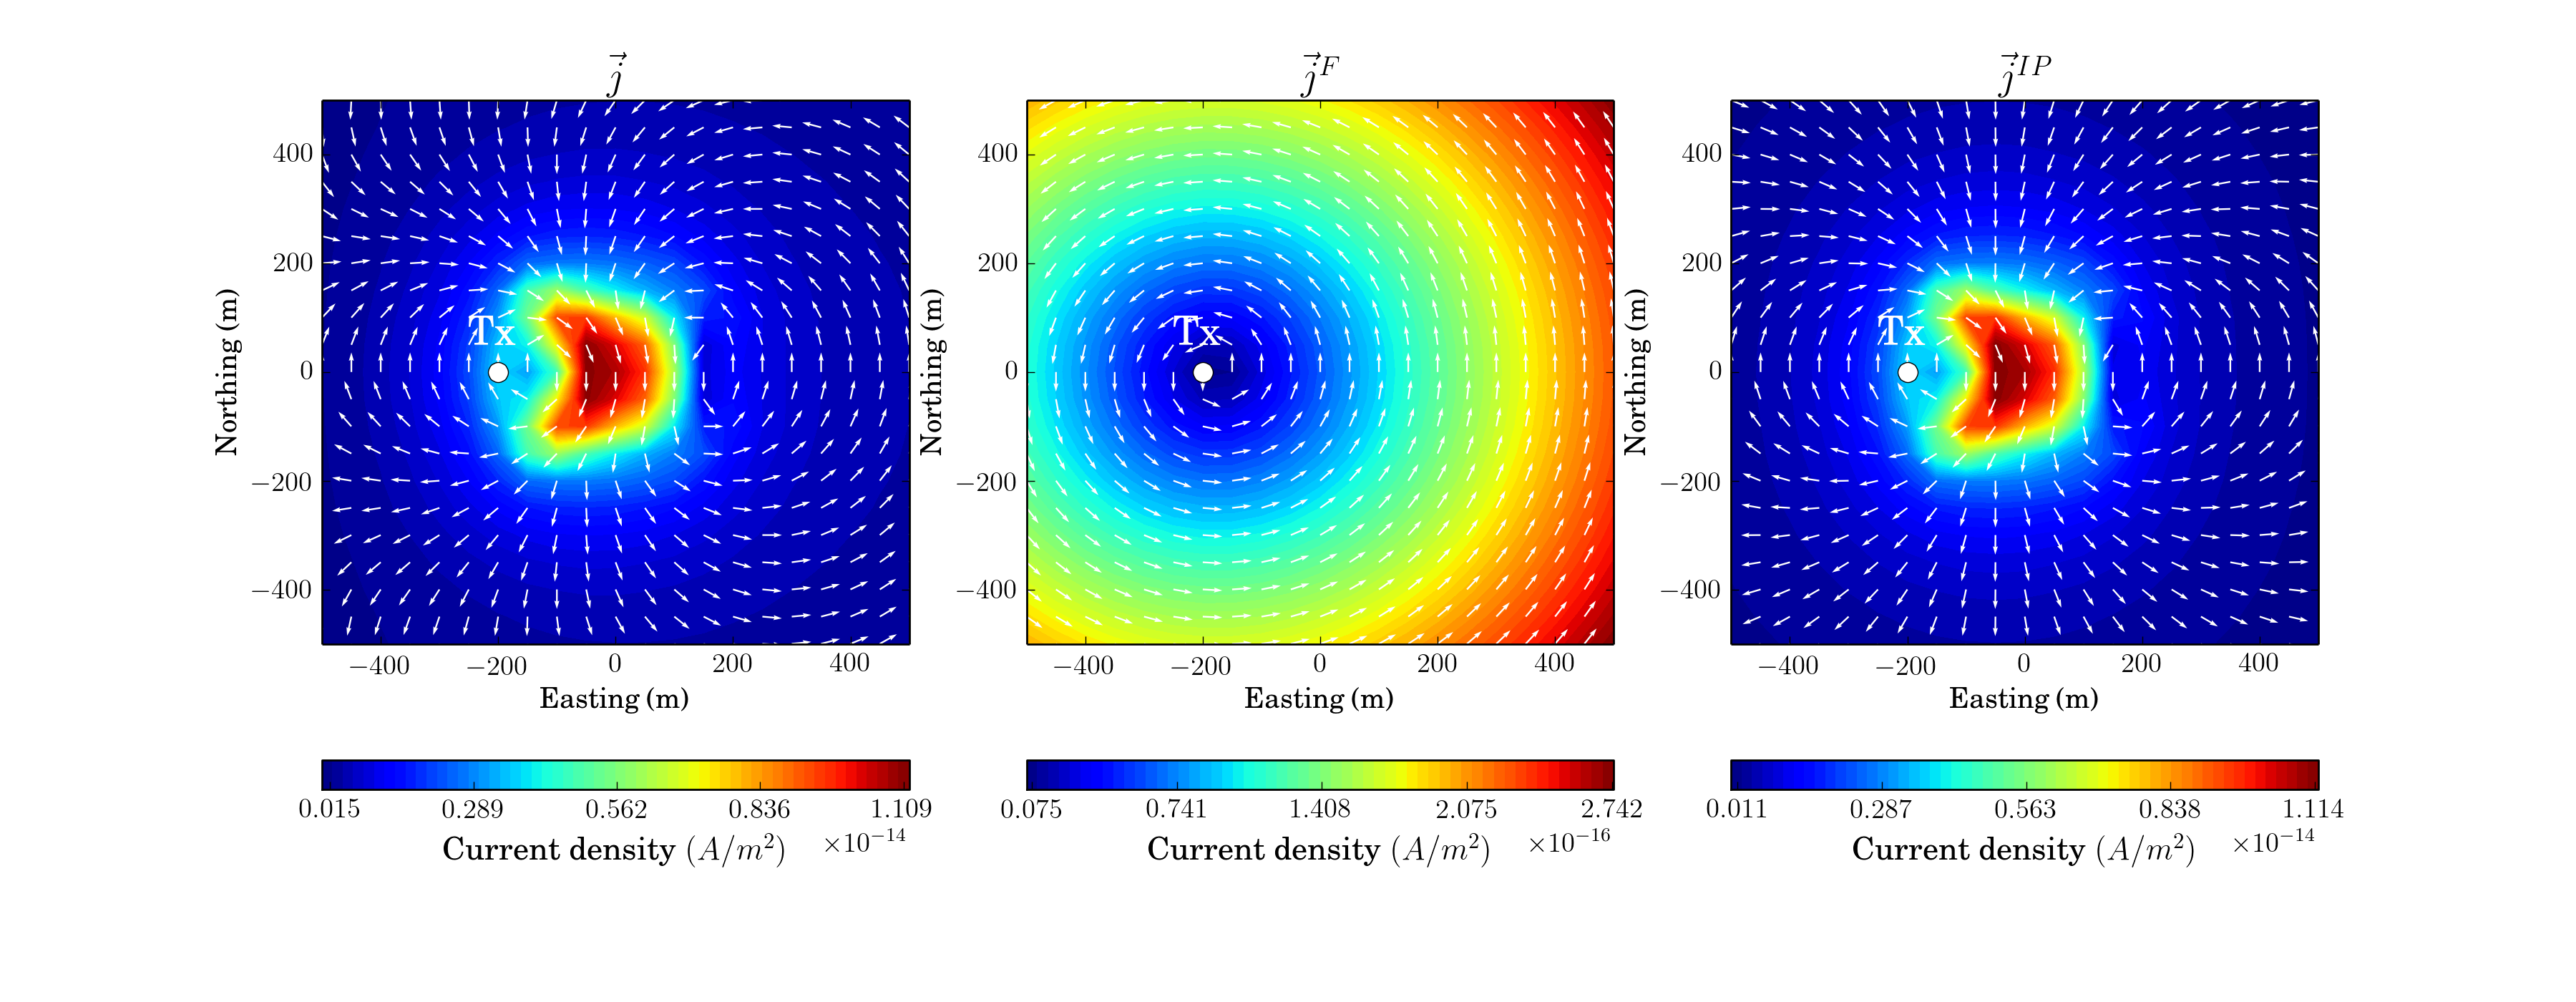
\includegraphics[height=0.25\textheight]{figures/synthetic/CurrentEMIP_case1_ch38.png} \\
  (b)
  \caption{Interpolated map of $\j$, $\j^F$ and $\j^{IP}$ at -175 m depth for canonical model. (a) Current densities at t=0.37 ms. (b)  Current densities at t=4.7 ms. }
  \label{F: currentEMIP_case1_plan}
\end{figure}

\begin{figure}[htb]
  \centering
  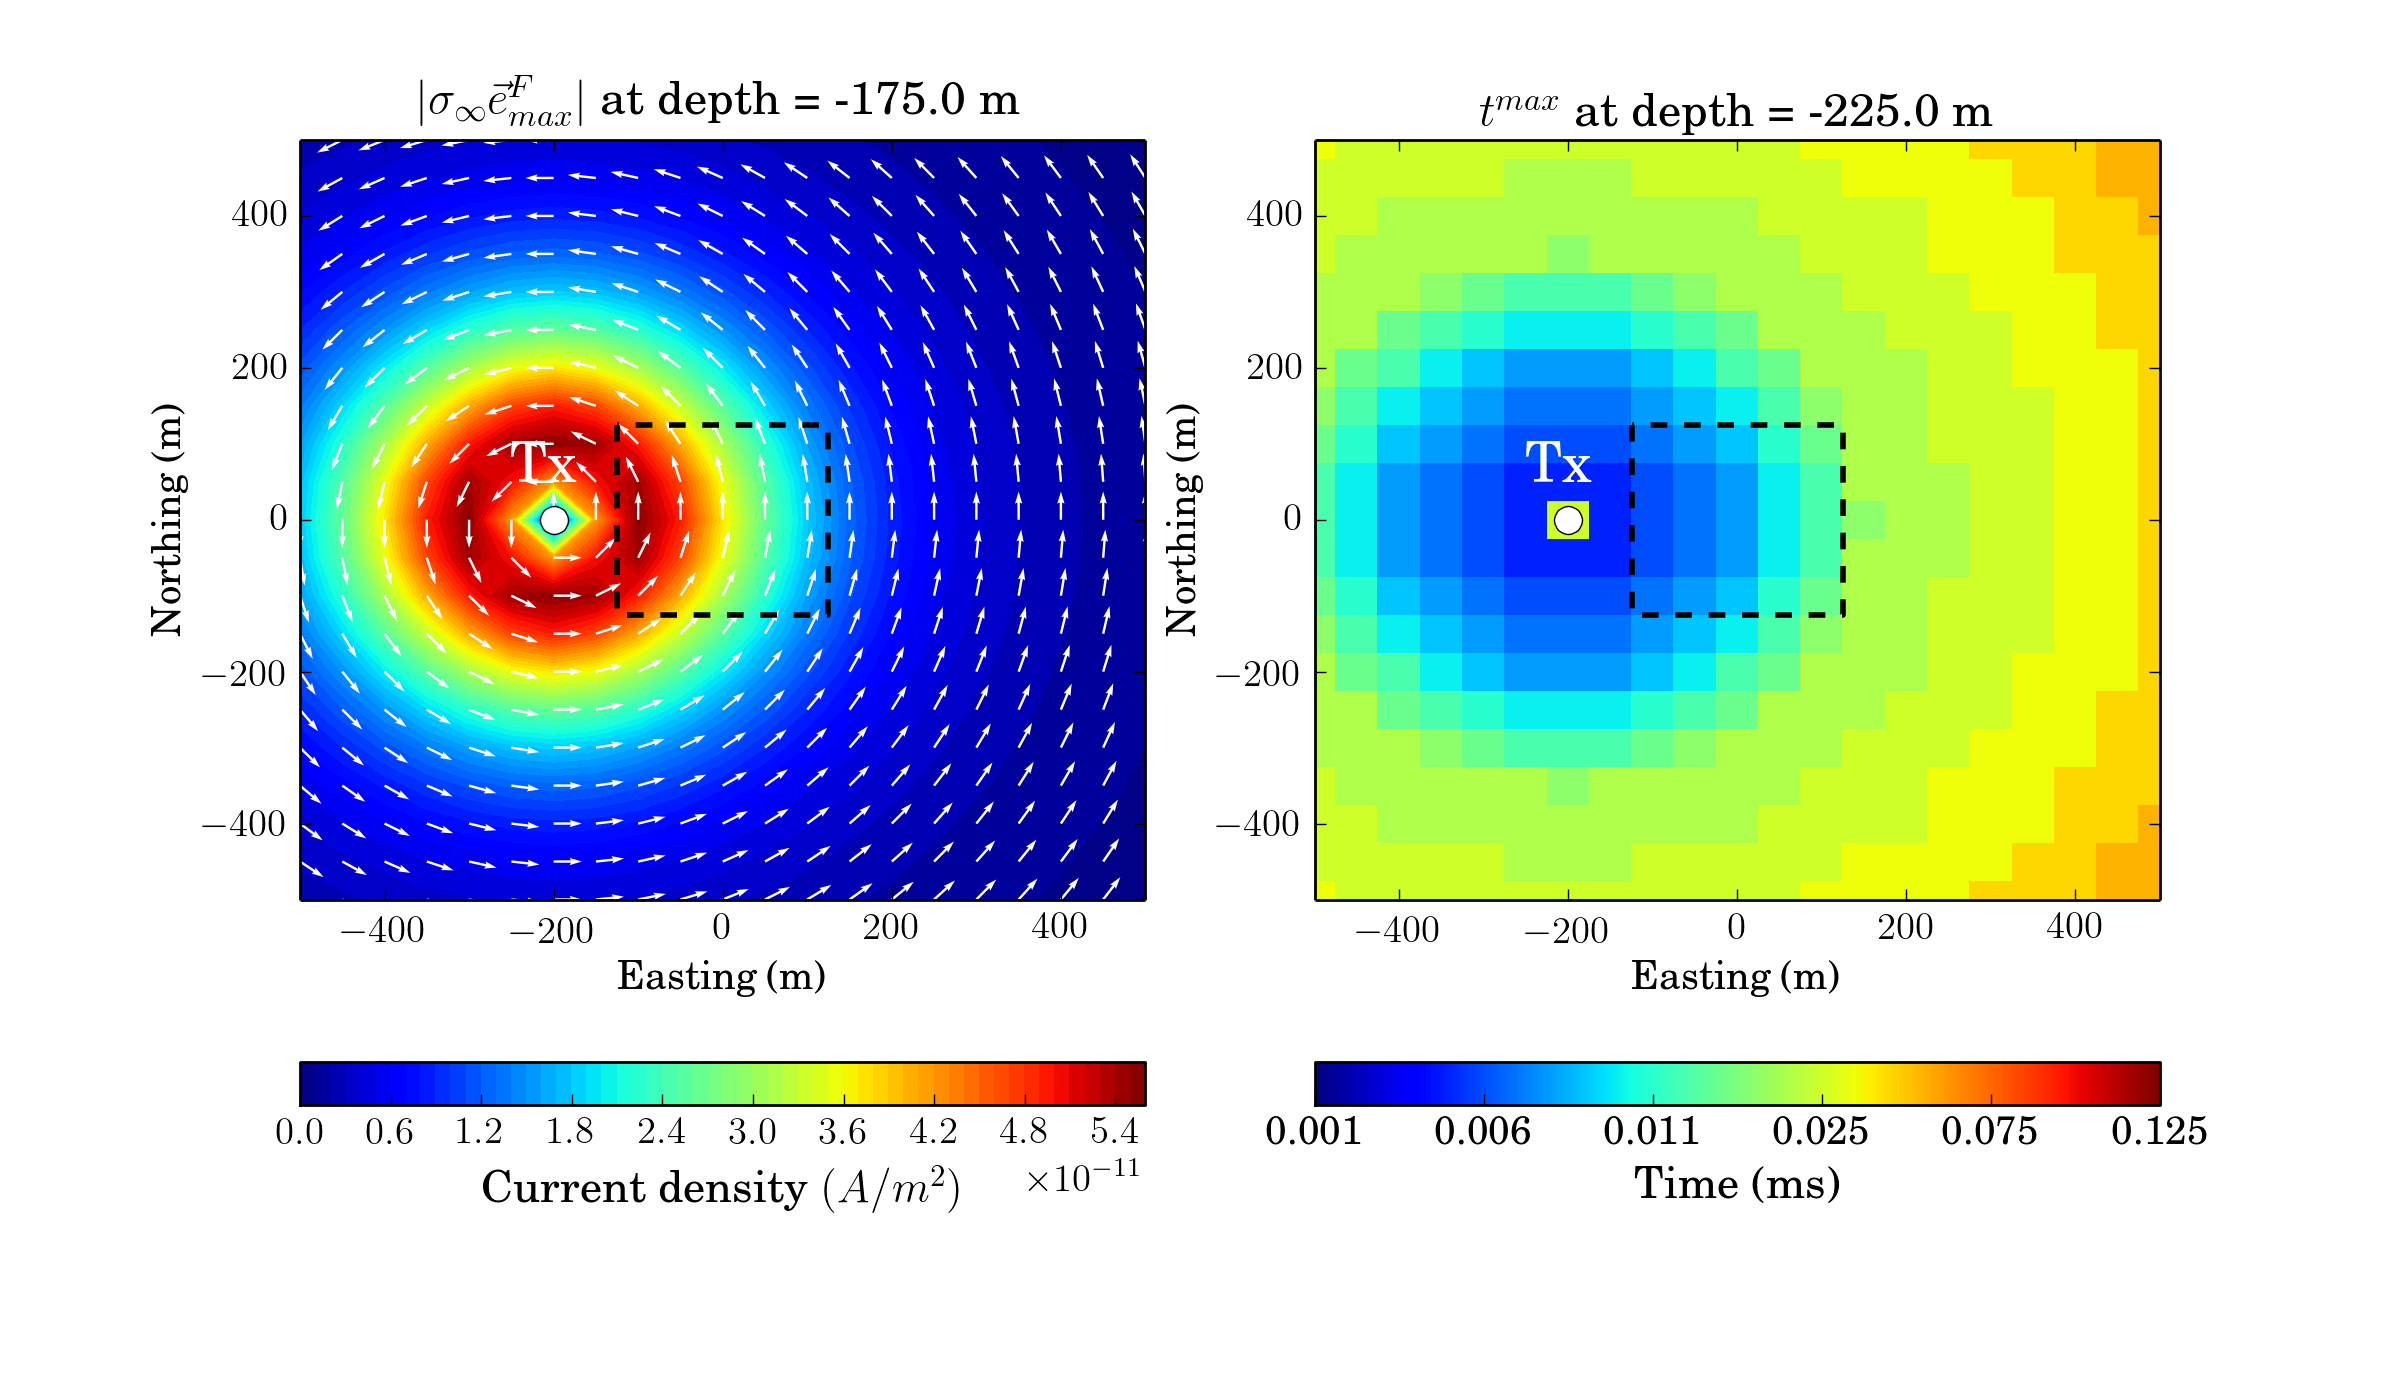
\includegraphics[height=0.4\textheight]{figures/synthetic/JmaxTmaxCase1_plan.png} \\
  \caption{Interpolated maps of $\siginf\e^F_{max}$ and $t^{max}$ at -175 m depth for canonical model. (a) $\siginf\e^F_{max}$ and (b) $t^{max}$.}
  \label{F: JmaxTmaxCase1_plan}
\end{figure}

\begin{figure}[htb]
  \centering
  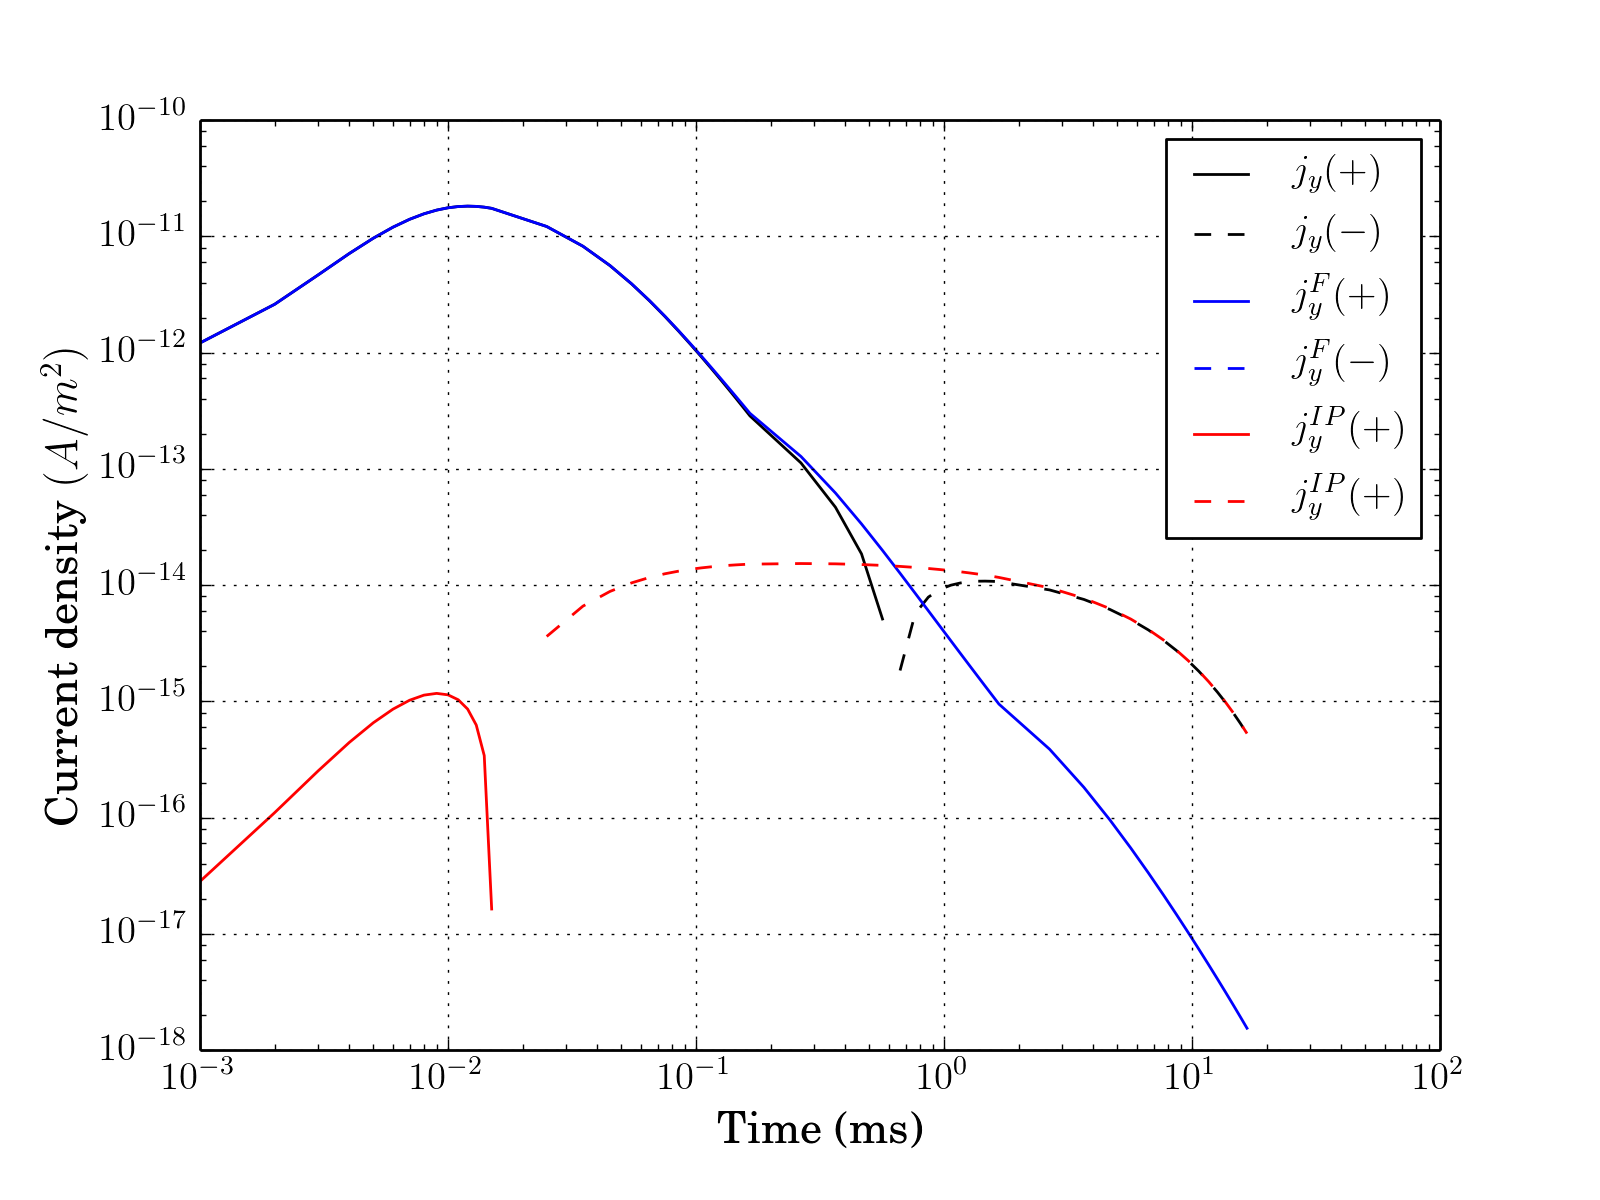
\includegraphics[height=0.4\textheight]{figures/synthetic/CurrentIP_case1_decay.png} \\
  (a) \\
  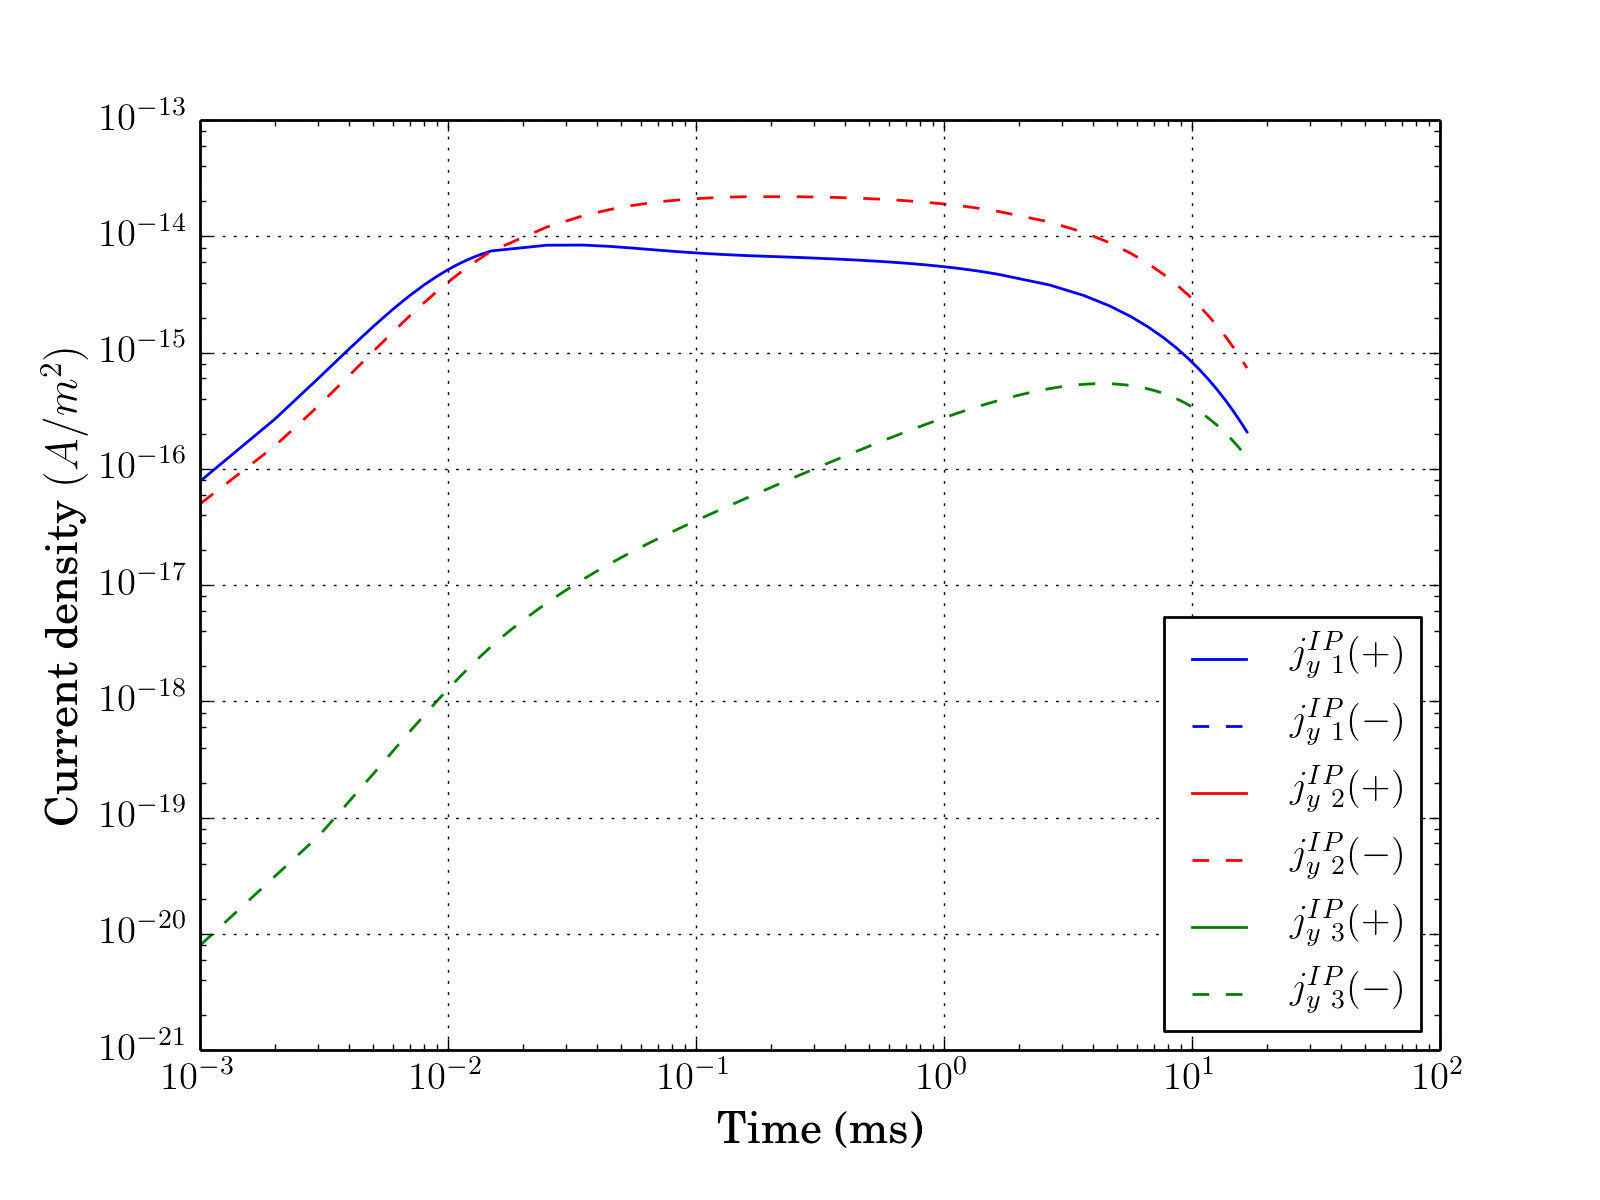
\includegraphics[height=0.4\textheight]{figures/synthetic/CurrentIP_decay_case1_2.png} \\
  (b)
  \caption{(a) Time decaying curves of current densities at Rx location for canonical model. (a) $\j_y$ (black), $\j^F_y$ (blue) and $\j^{IP}_y$ (red). (b) $\j^{IP}_{y \ 1}$ (blue), $\j^{IP}_{y \ 2}$ (red) and $\j^{IP}_{y \ 3}$ (green).}
  \label{F: currentEMIP_case1_decay}
\end{figure}

\begin{figure}[htb]
  \centering
  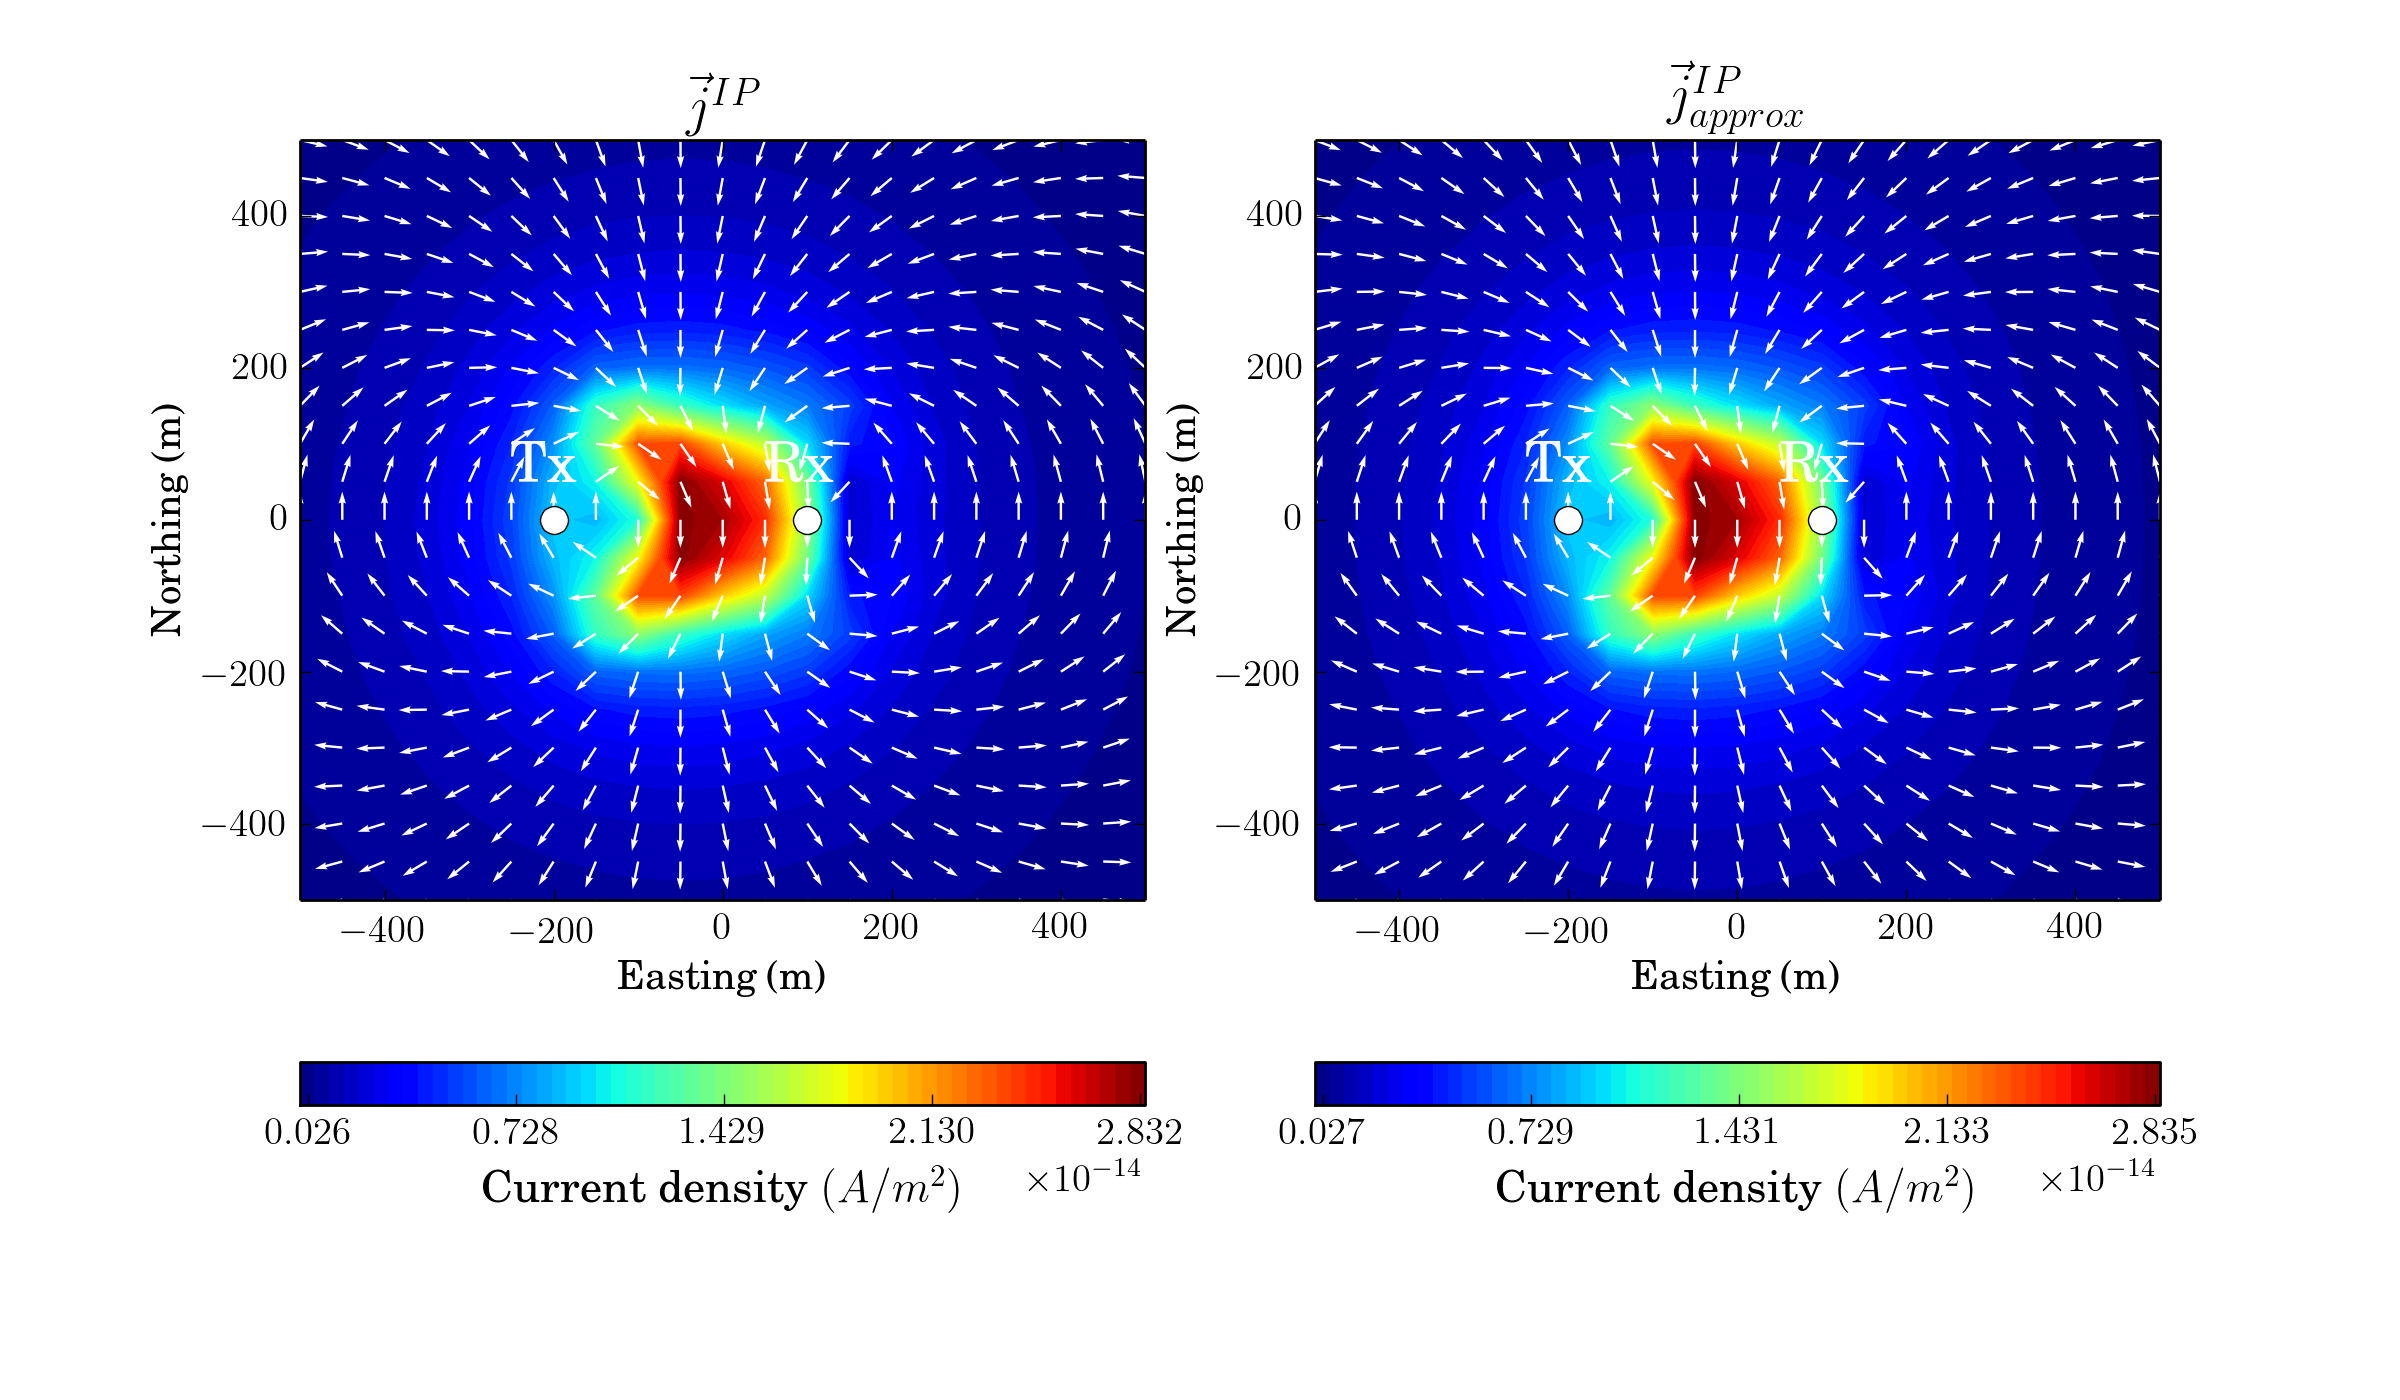
\includegraphics[height=0.4\textheight]{figures/synthetic/CurrentIP_case1_ch20.png} \\
  (a) \\
  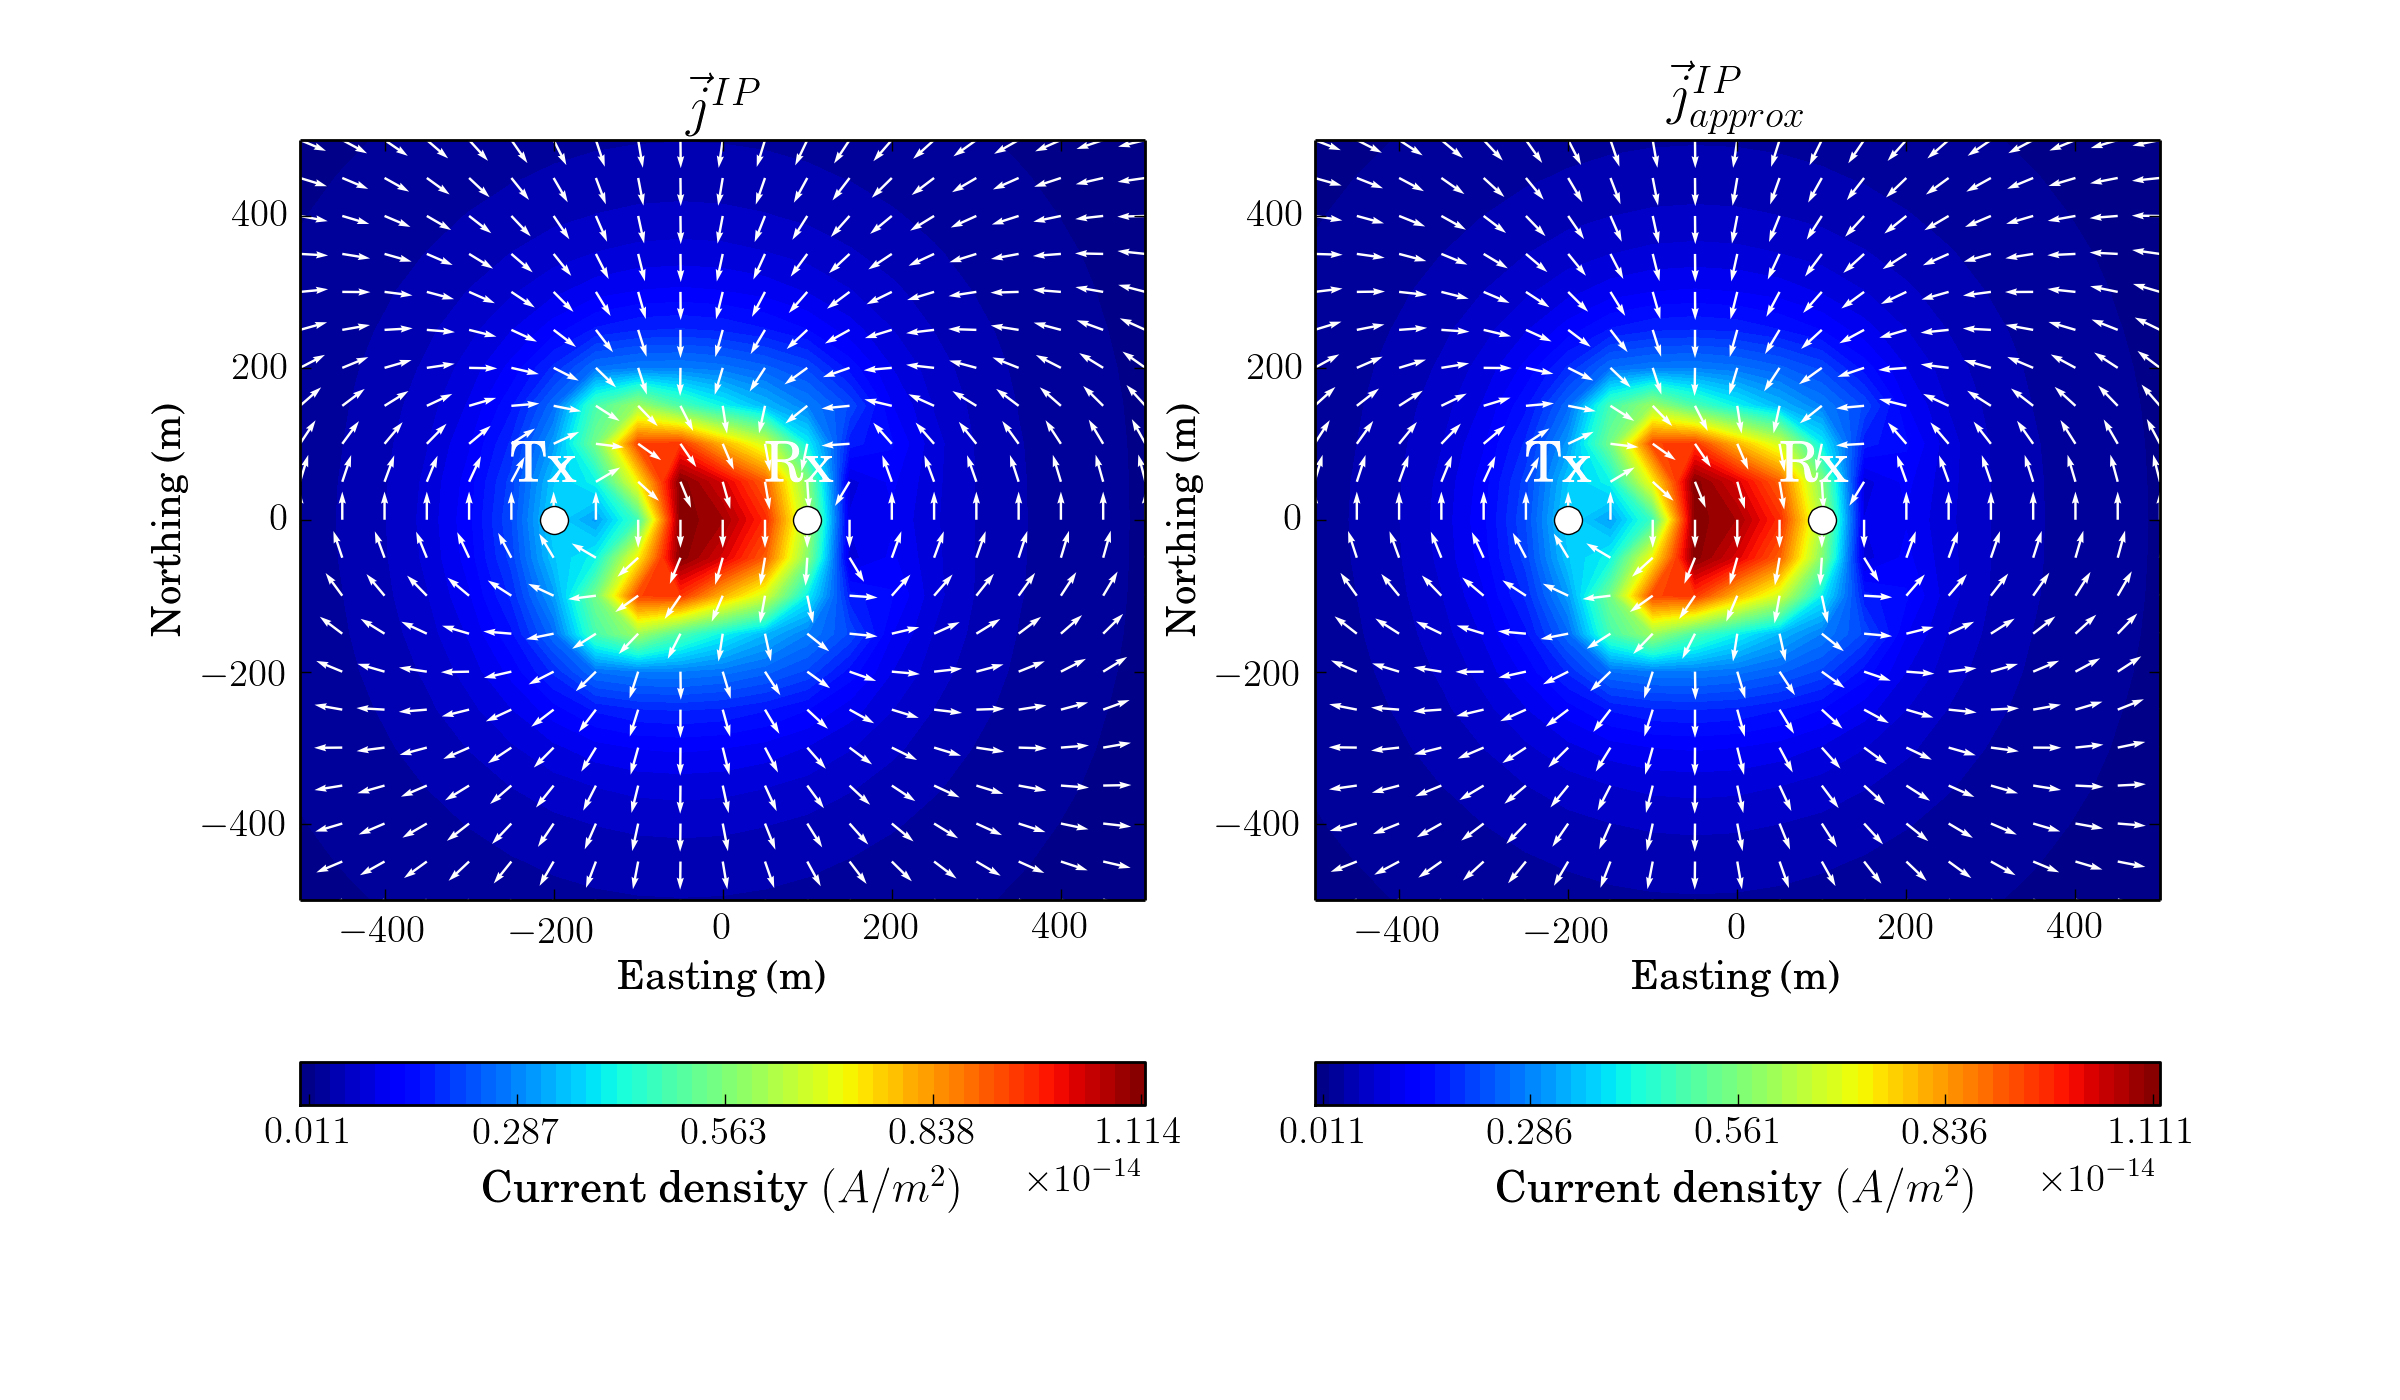
\includegraphics[height=0.4\textheight]{figures/synthetic/CurrentIP_case1_ch38.png} \\
  (b)
  \caption{Interpolated maps of $\j^{IP}$ and $\j^{IP}_{approx}$ at -175 m depth for canonical model. (a) t=0.37 ms and (b) t=4.7 ms.}
  \label{F: currentIP_case1_plan}
\end{figure}

\begin{figure}[htb]
  \centering
  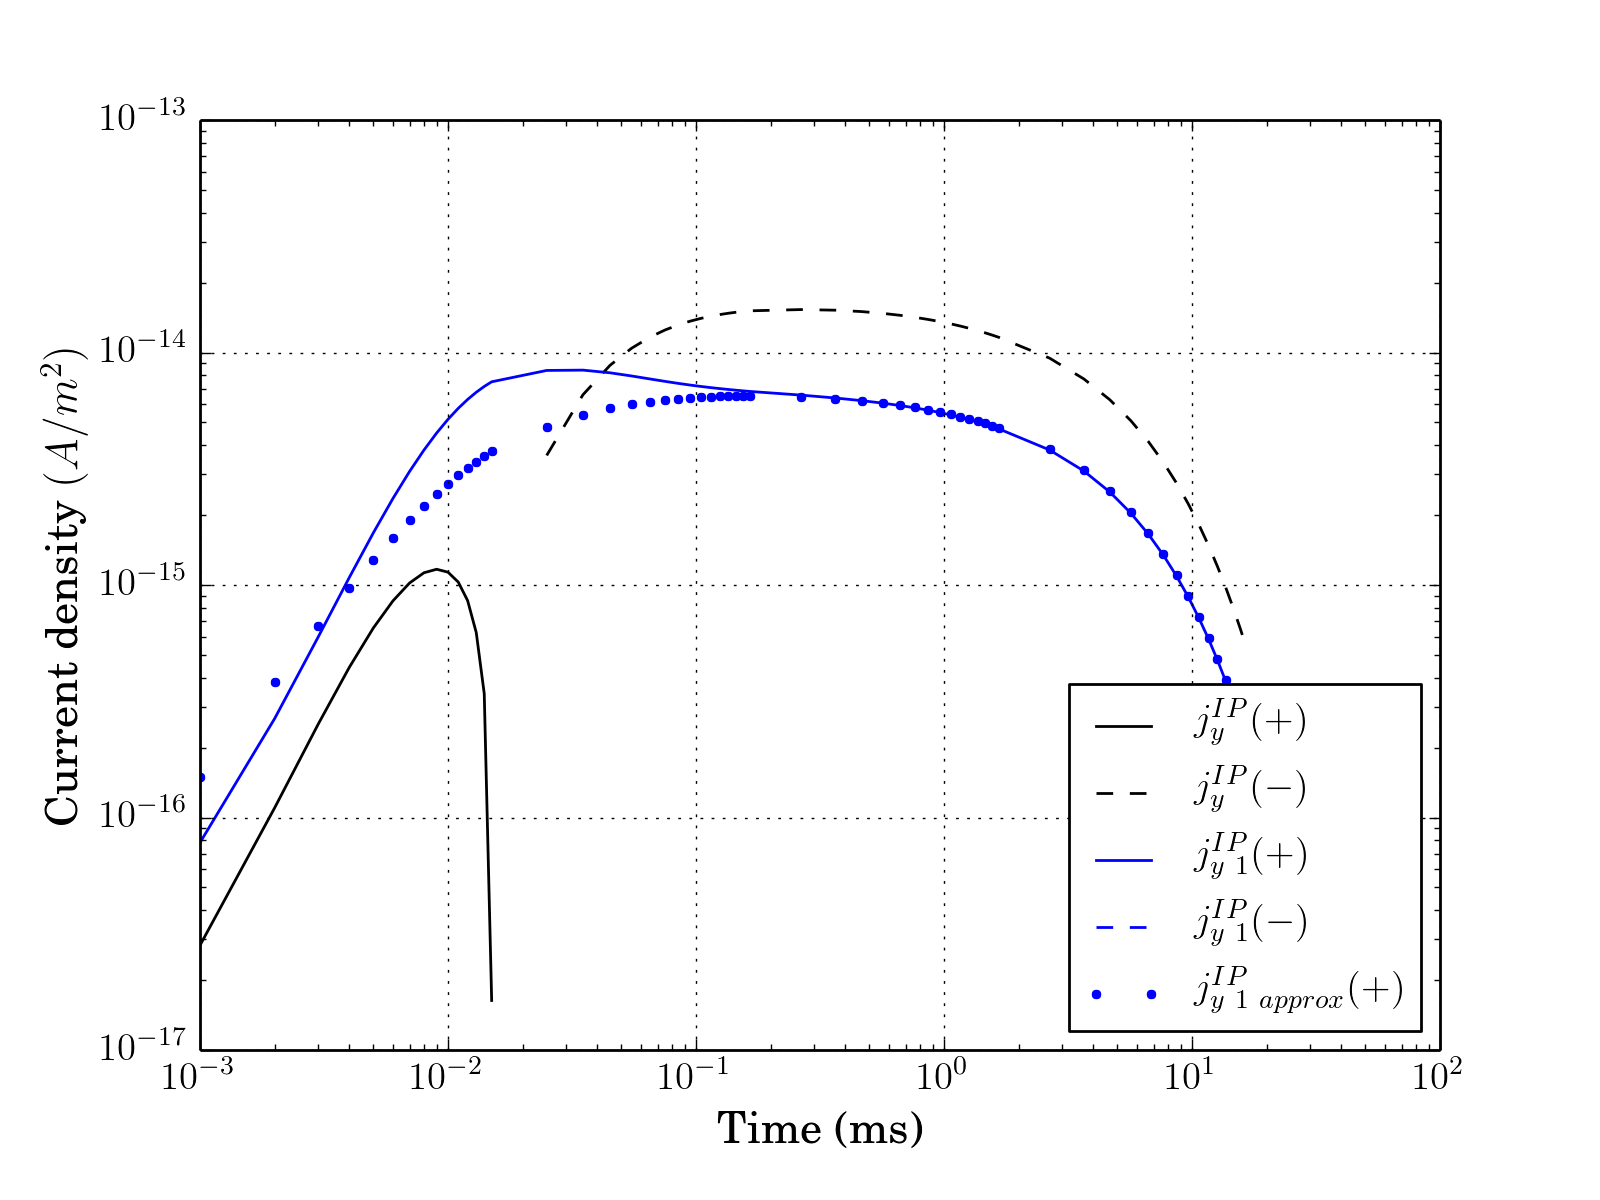
\includegraphics[height=0.4\textheight]{figures/synthetic/CurrentIP_decay_case1_1.png} \\
  \caption{Time decaying curves of $j_y^{IP}$ (black), $j_{y \ 1}^{IP}$ (blue) and $j_{y \ 1 \ approx}^{IP}$ (blue dots) at Rx location for canonical model. }
  \label{F: currentIP_case1_decay}
\end{figure}
\clearpage
\begin{figure}[htb]
  \centering
  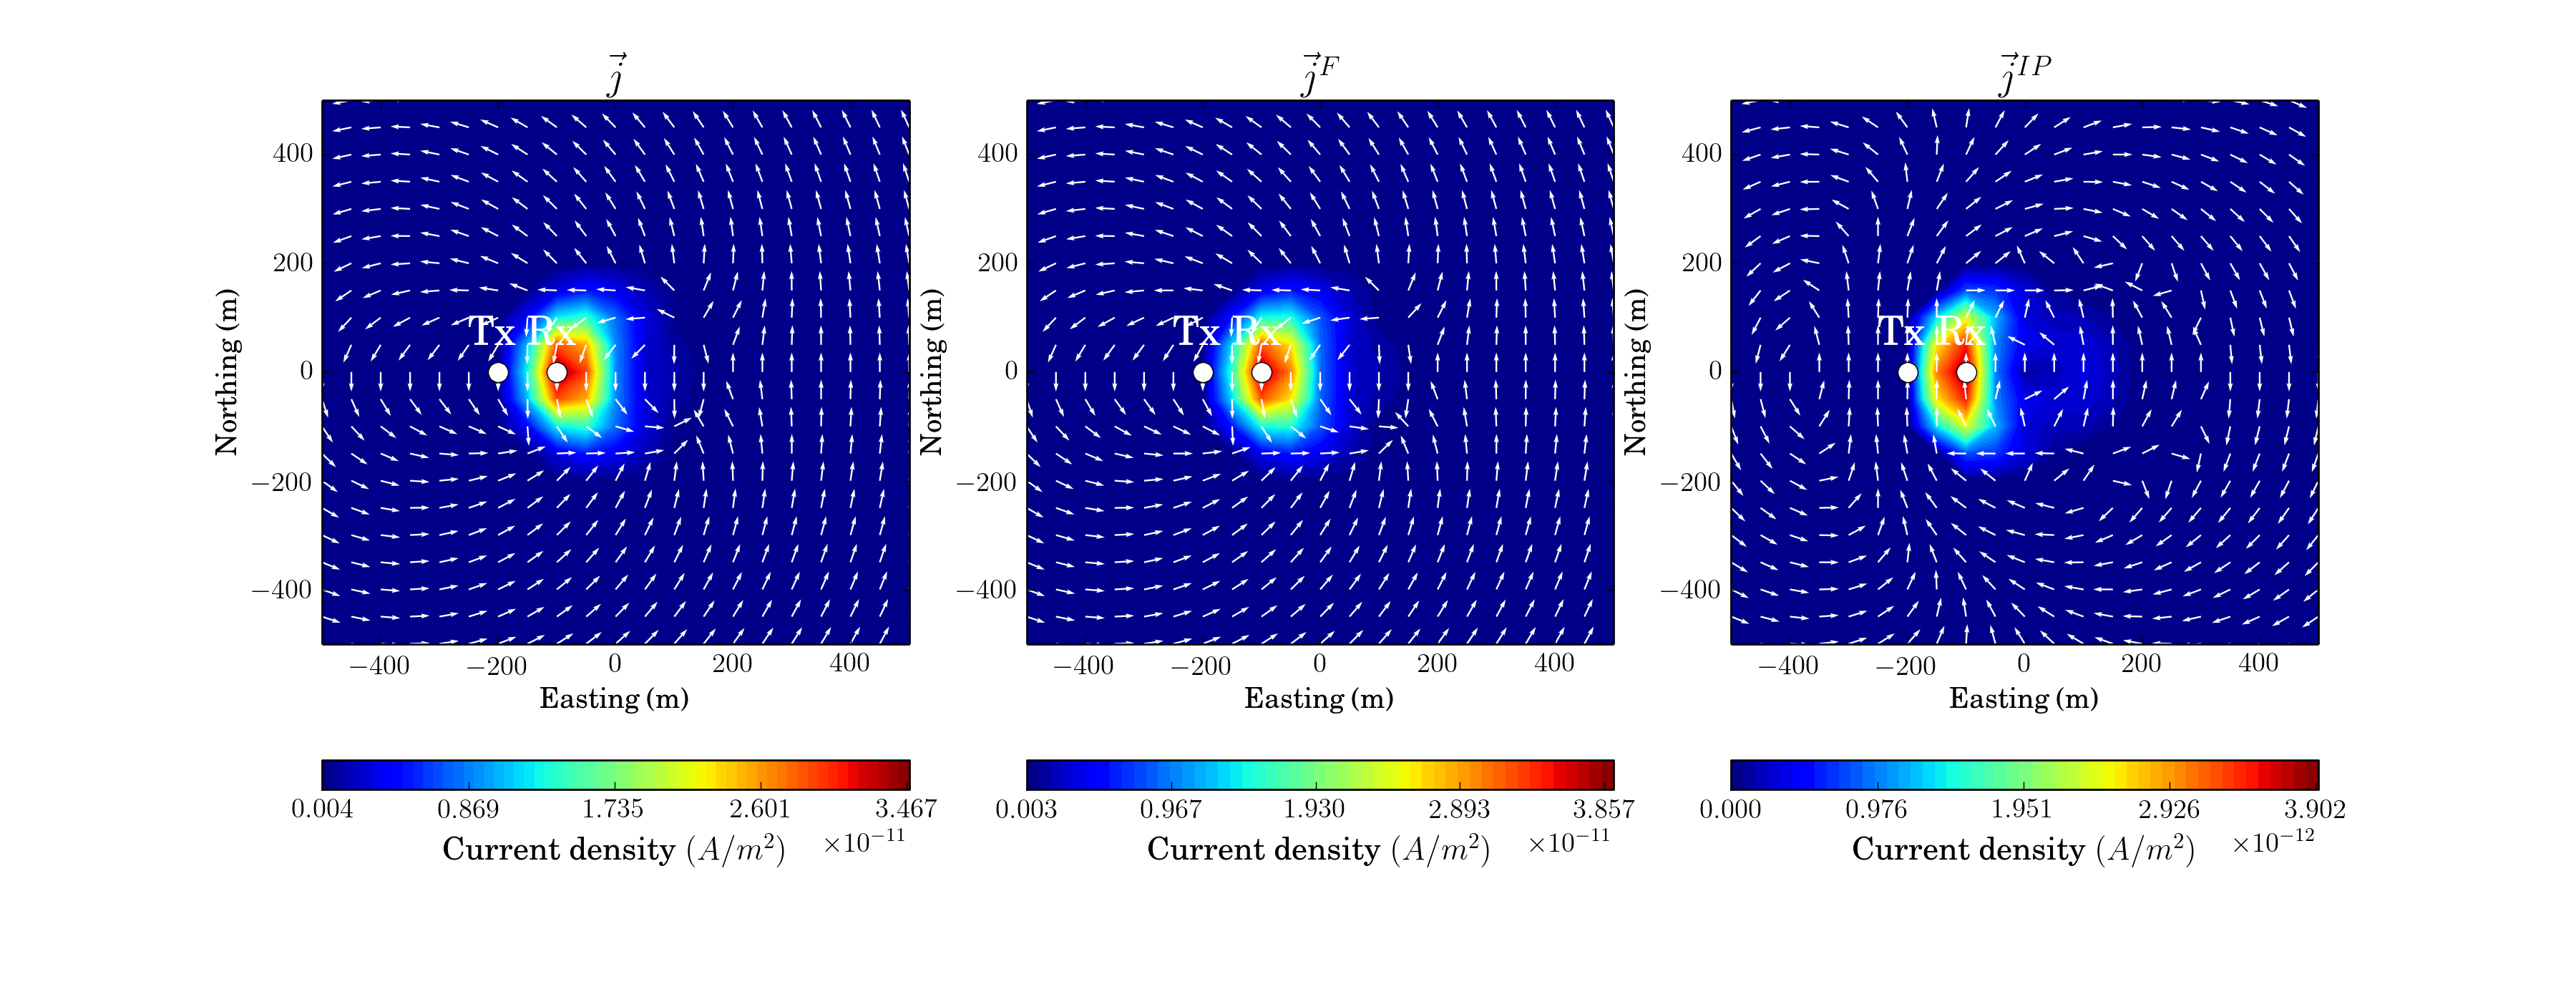
\includegraphics[height=0.25\textheight]{figures/synthetic/CurrentEMIP_case2_ch20.png} \\
  (a) \\
  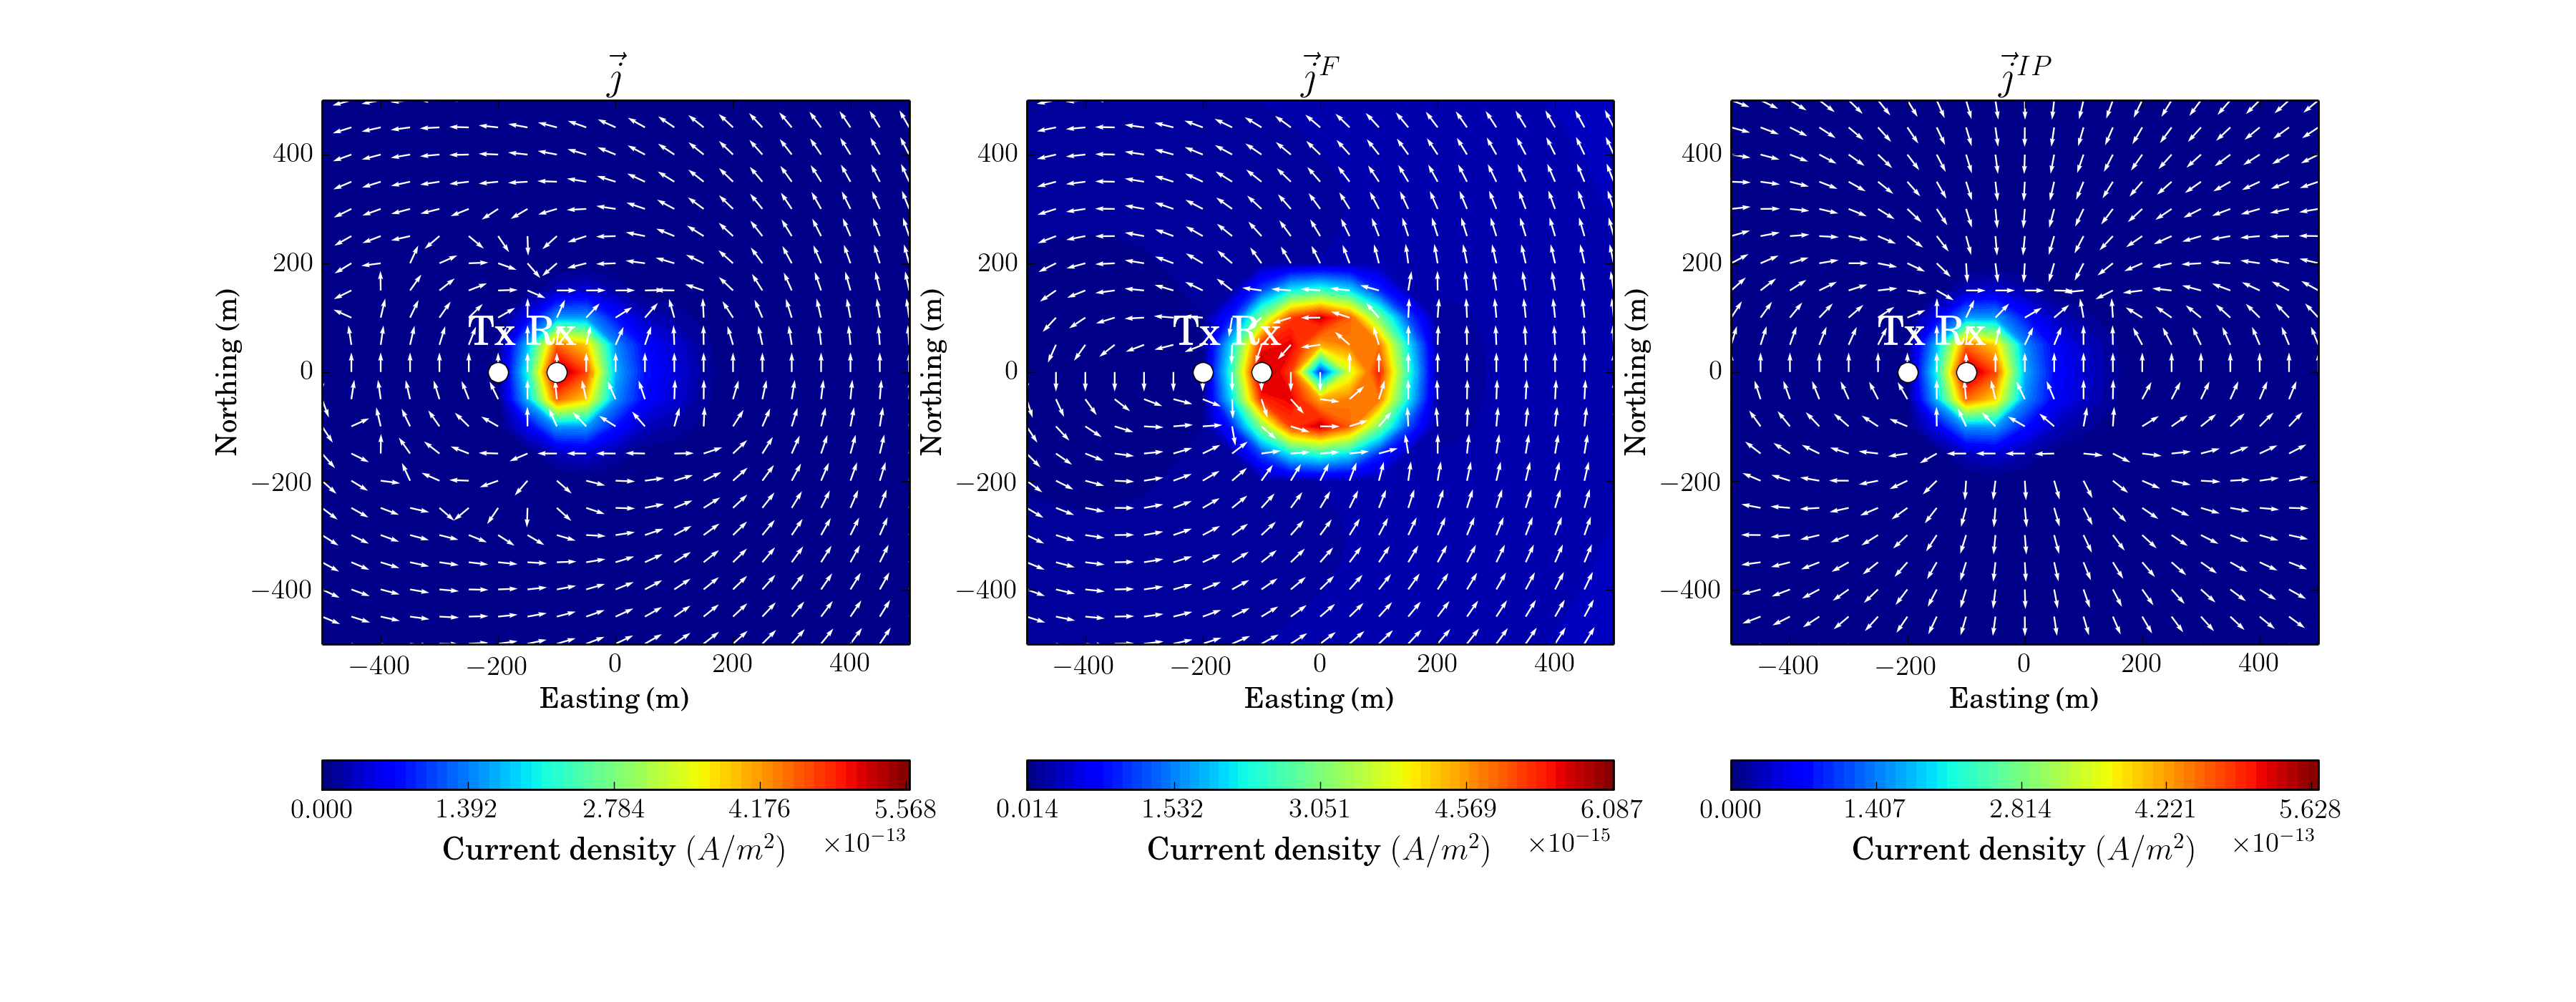
\includegraphics[height=0.25\textheight]{figures/synthetic/CurrentEMIP_case2_ch38.png} \\
  (b)
  \caption{Interpolated map of $\j$, $\j^F$ and $\j^{IP}$ at -175 m depth for Conductive     model. (a) Current densities at t=0.37 ms. (b)  Current densities at t=4.7 ms. }
  \label{F: currentEMIP_case2_plan}
\end{figure}

\begin{figure}[htb]
  \centering
  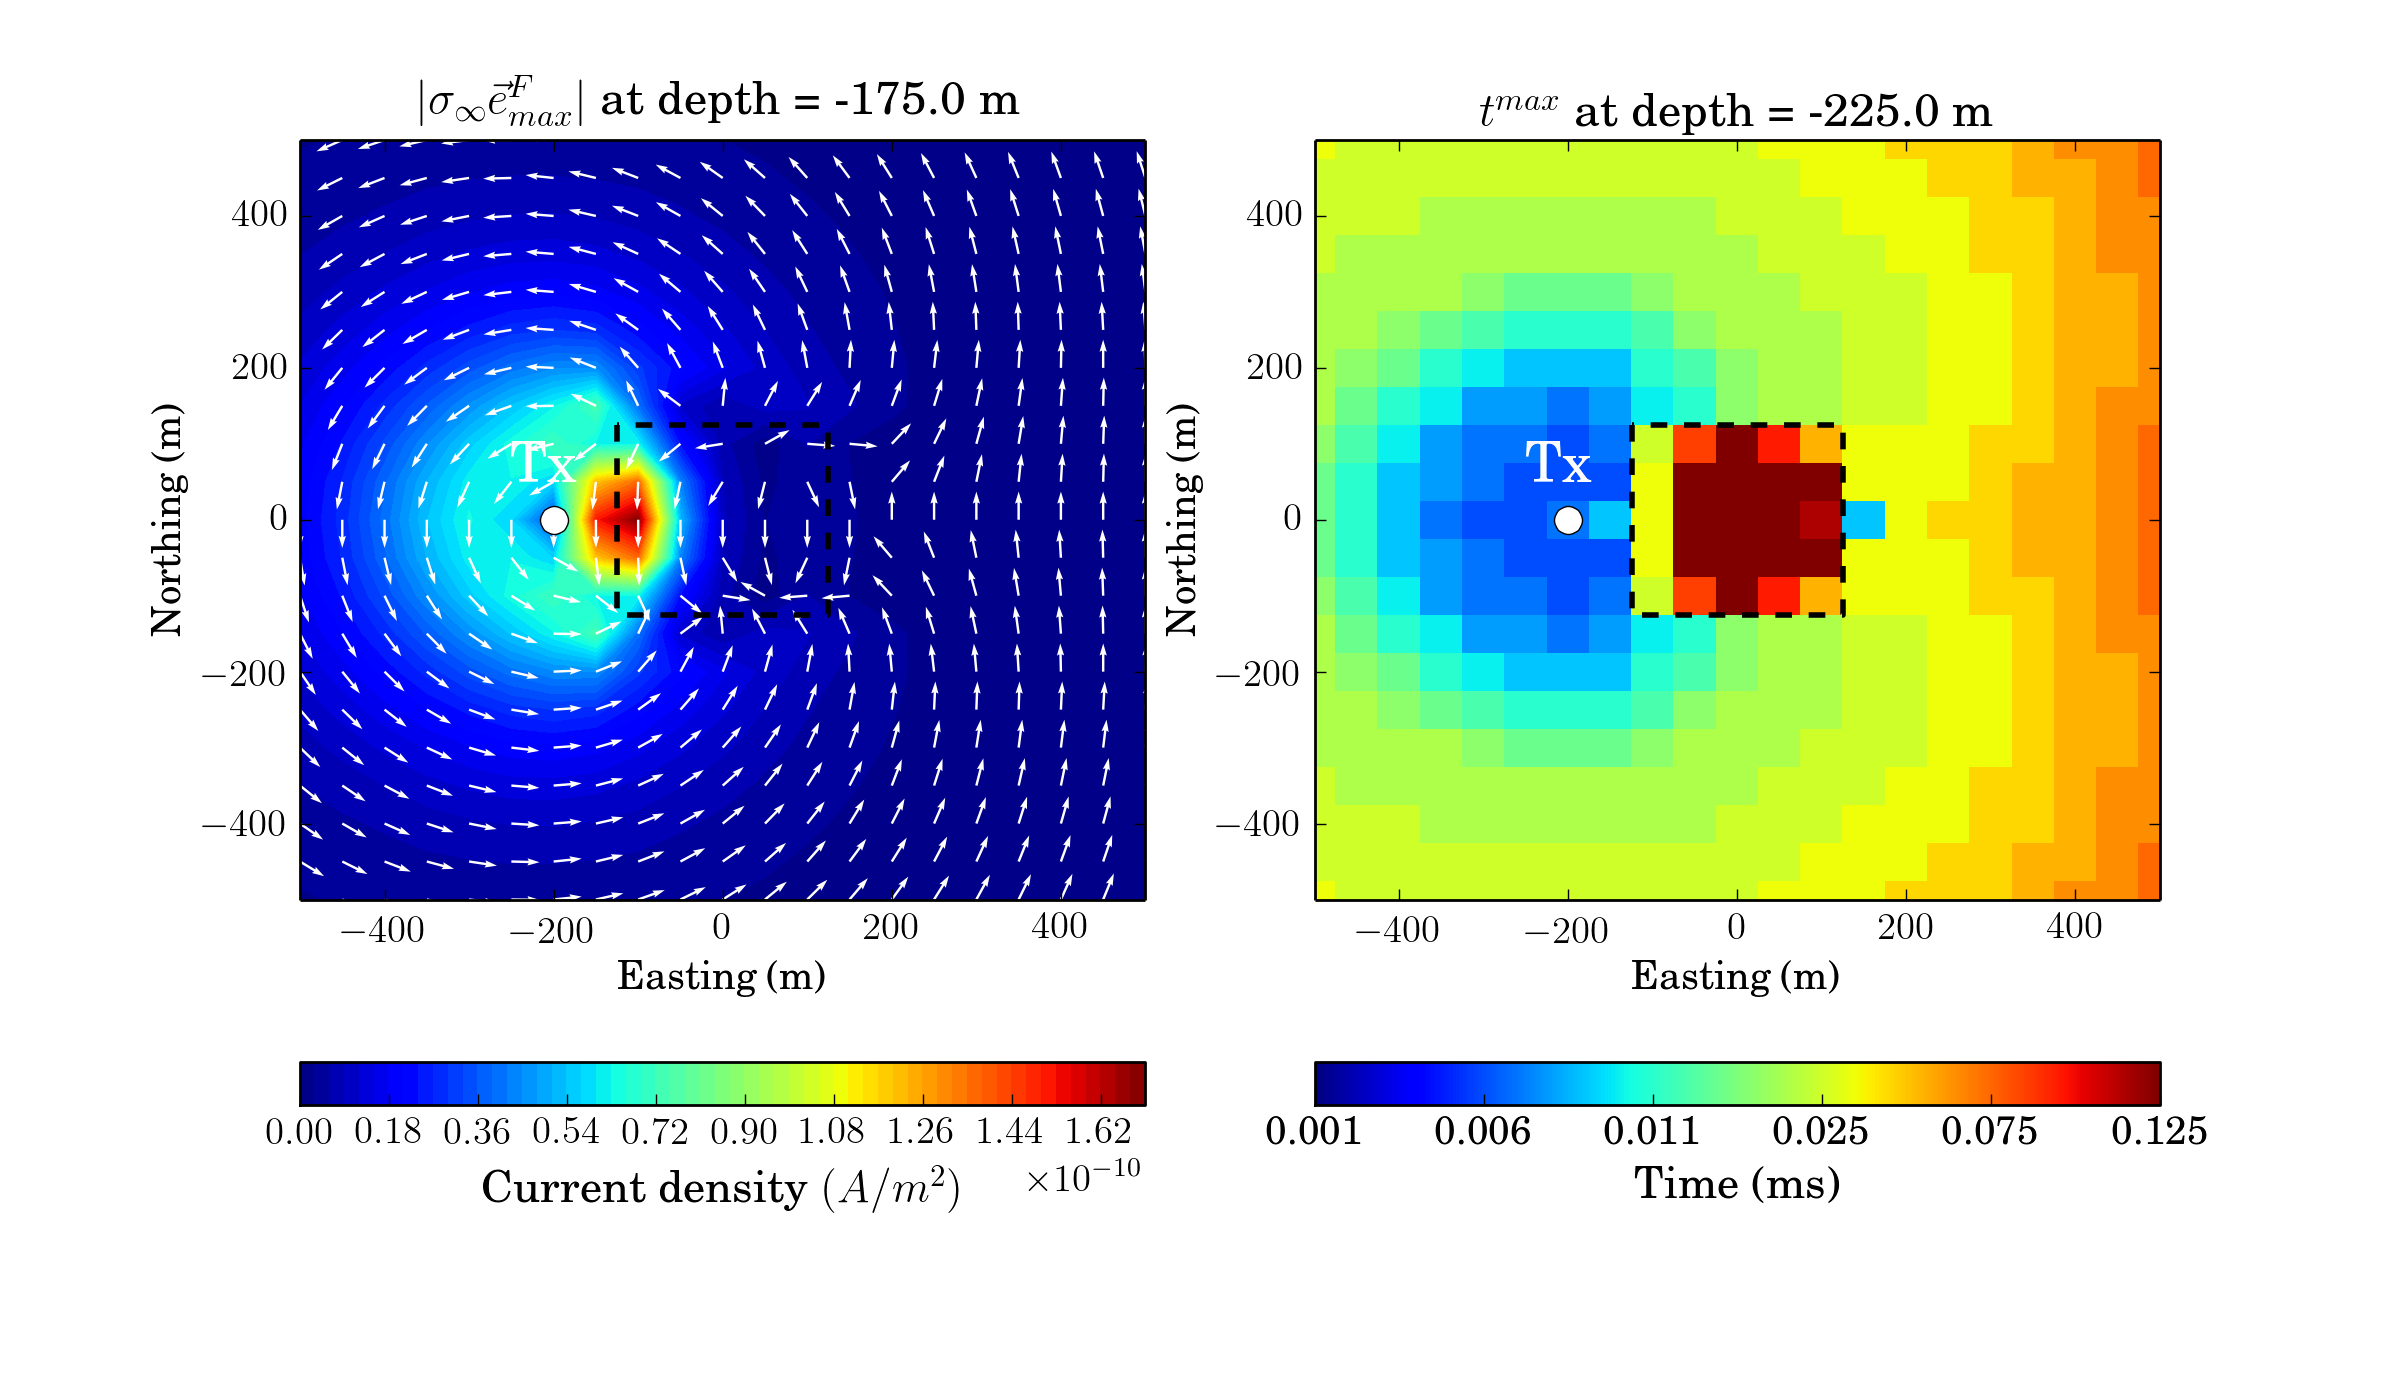
\includegraphics[height=0.4\textheight]{figures/synthetic/JmaxTmaxCase2_plan.png} \\
  \caption{Interpolated maps of $\siginf\e^F_{max}$ and $t^{max}$ at -175 m depth for conductive model. (a) $\siginf\e^F_{max}$ and (b) $t^{max}$.}
  \label{F: JmaxTmaxCase2_plan}
\end{figure}

\begin{figure}[htb]
  \centering
  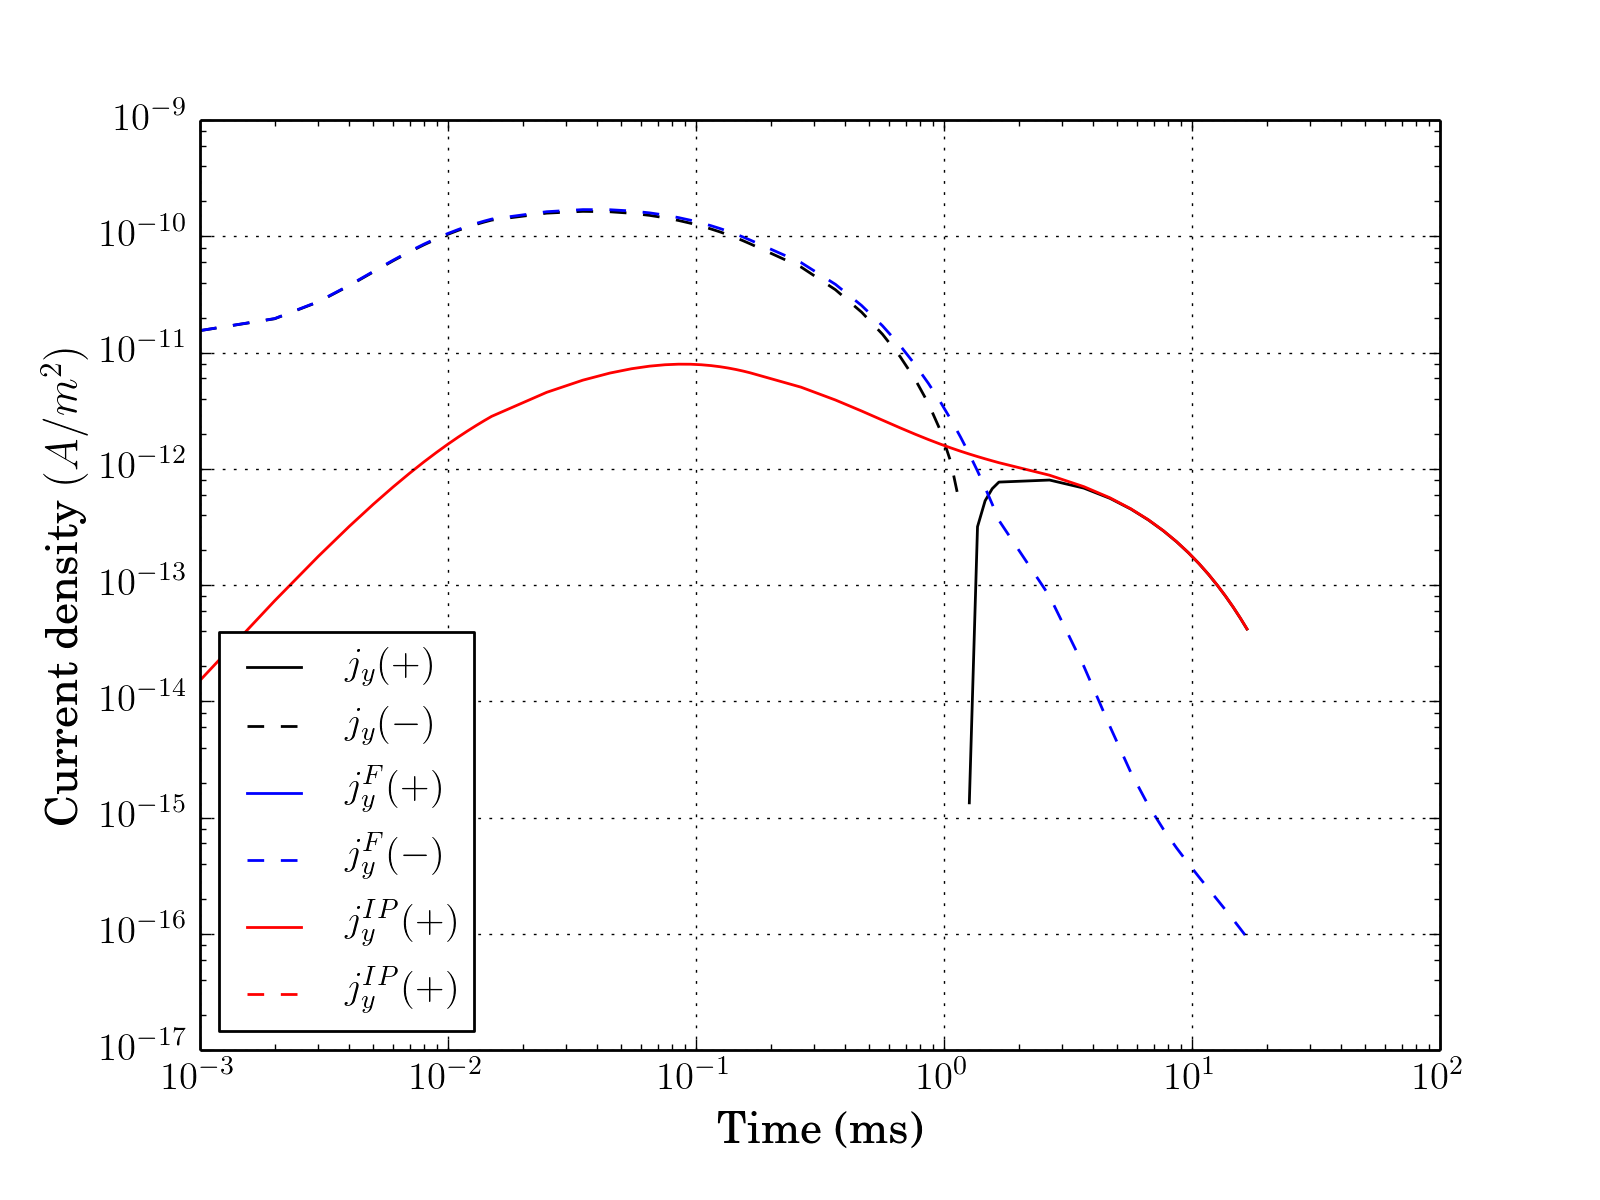
\includegraphics[height=0.4\textheight]{figures/synthetic/CurrentIP_case2_decay.png} \\
  (a) \\
  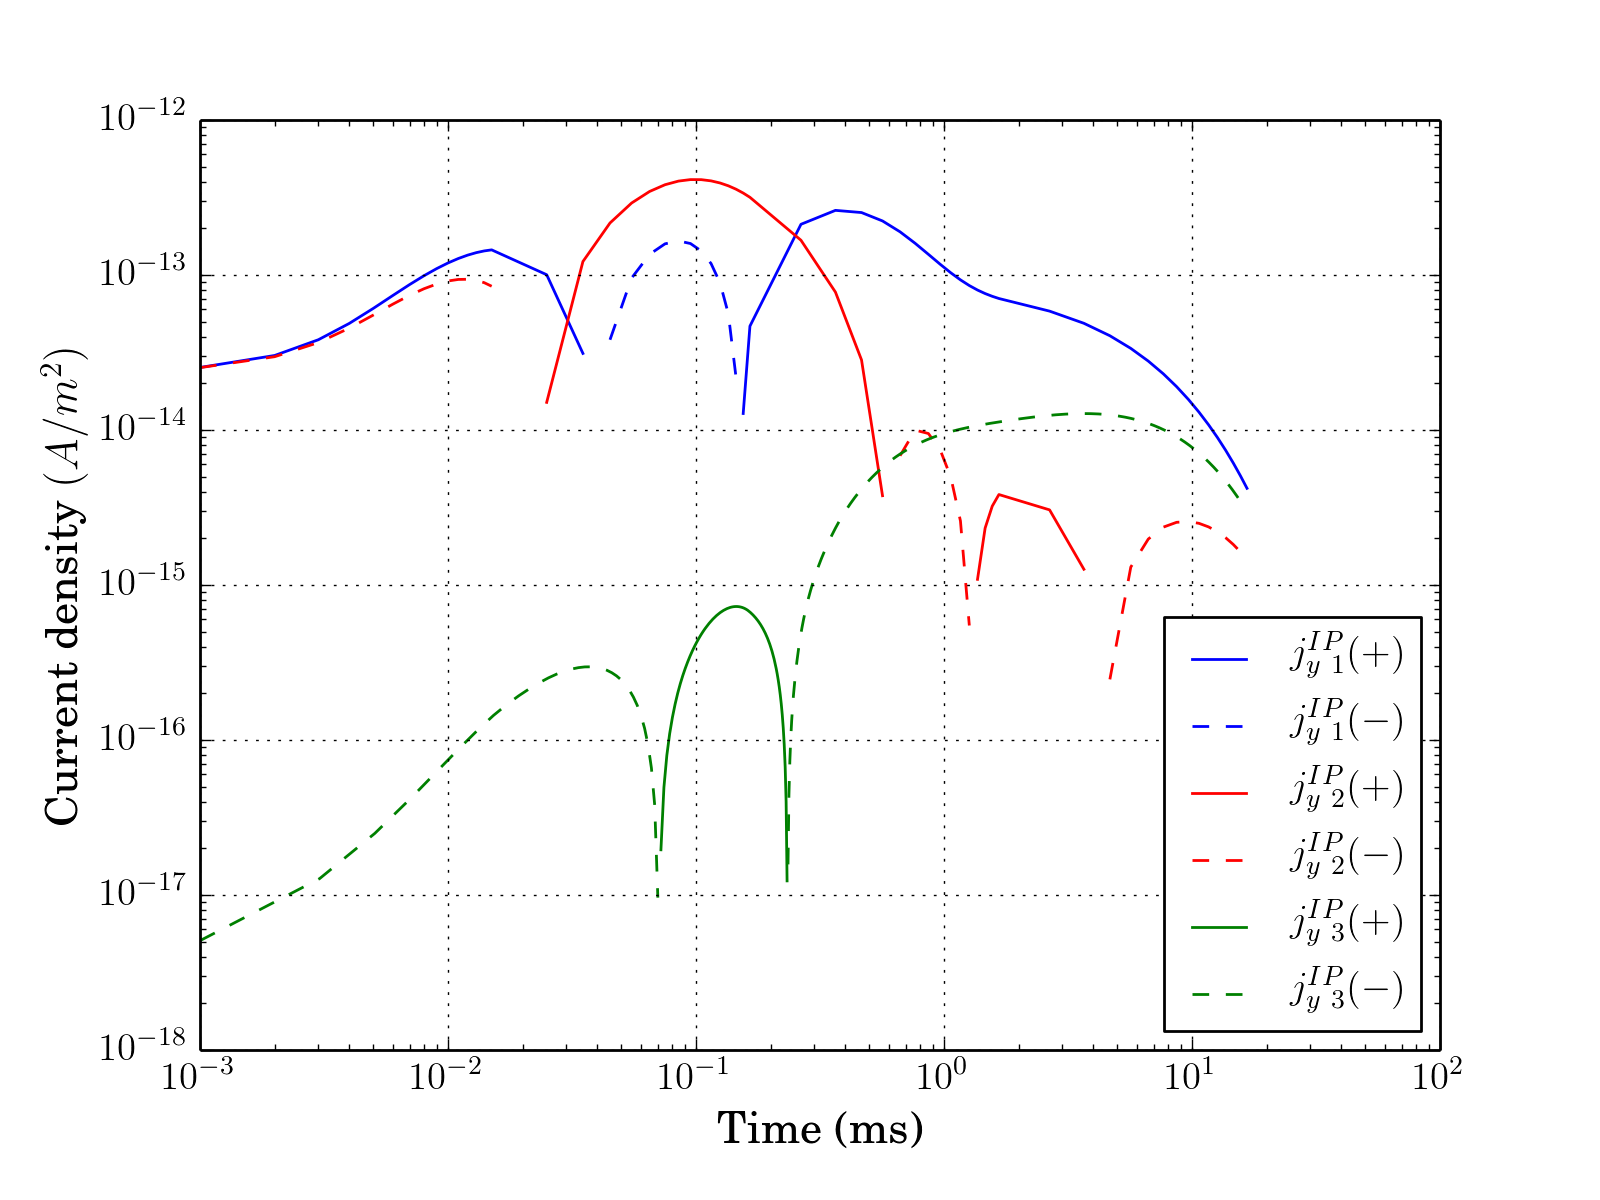
\includegraphics[height=0.4\textheight]{figures/synthetic/CurrentIP_decay_case2_2.png} \\
  (b)
  \caption{Time decaying curves of $\j_y$ (black), $\j^F_y$ (blue) and $\j^{IP}_y$ (red) at Rx location.}
  \label{F: currentEMIP_case2_decay}
\end{figure}

\begin{figure}[htb]
  \centering
  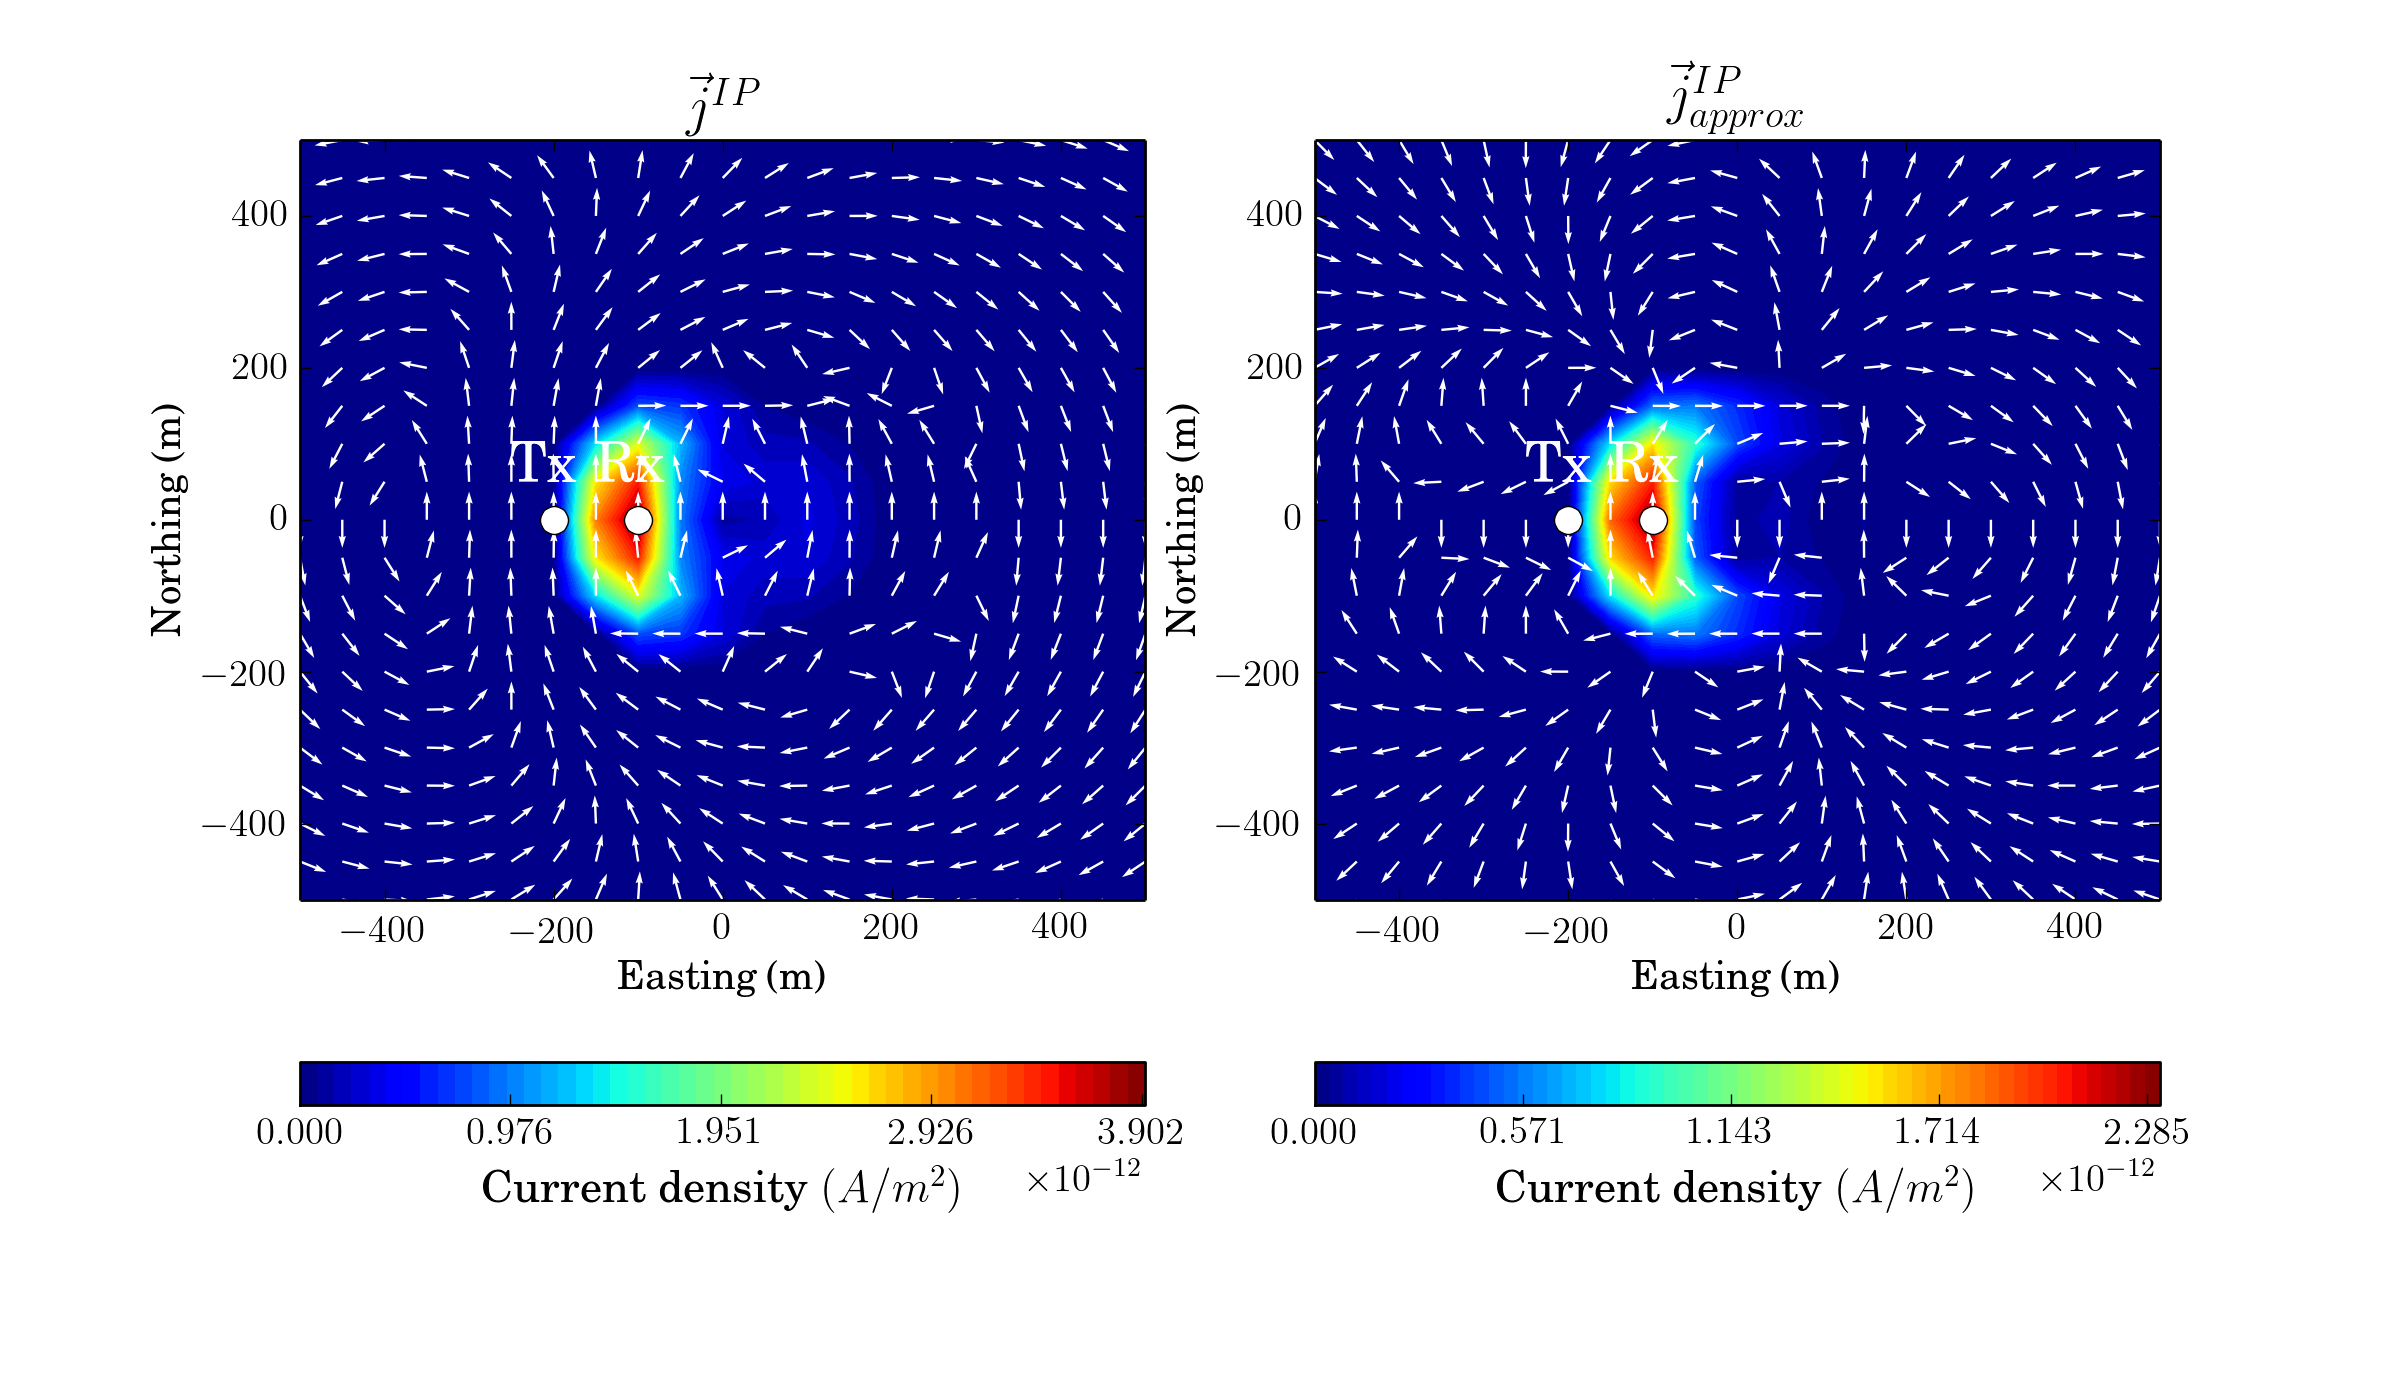
\includegraphics[height=0.4\textheight]{figures/synthetic/CurrentIP_case2_ch20.png} \\
  (a) \\
  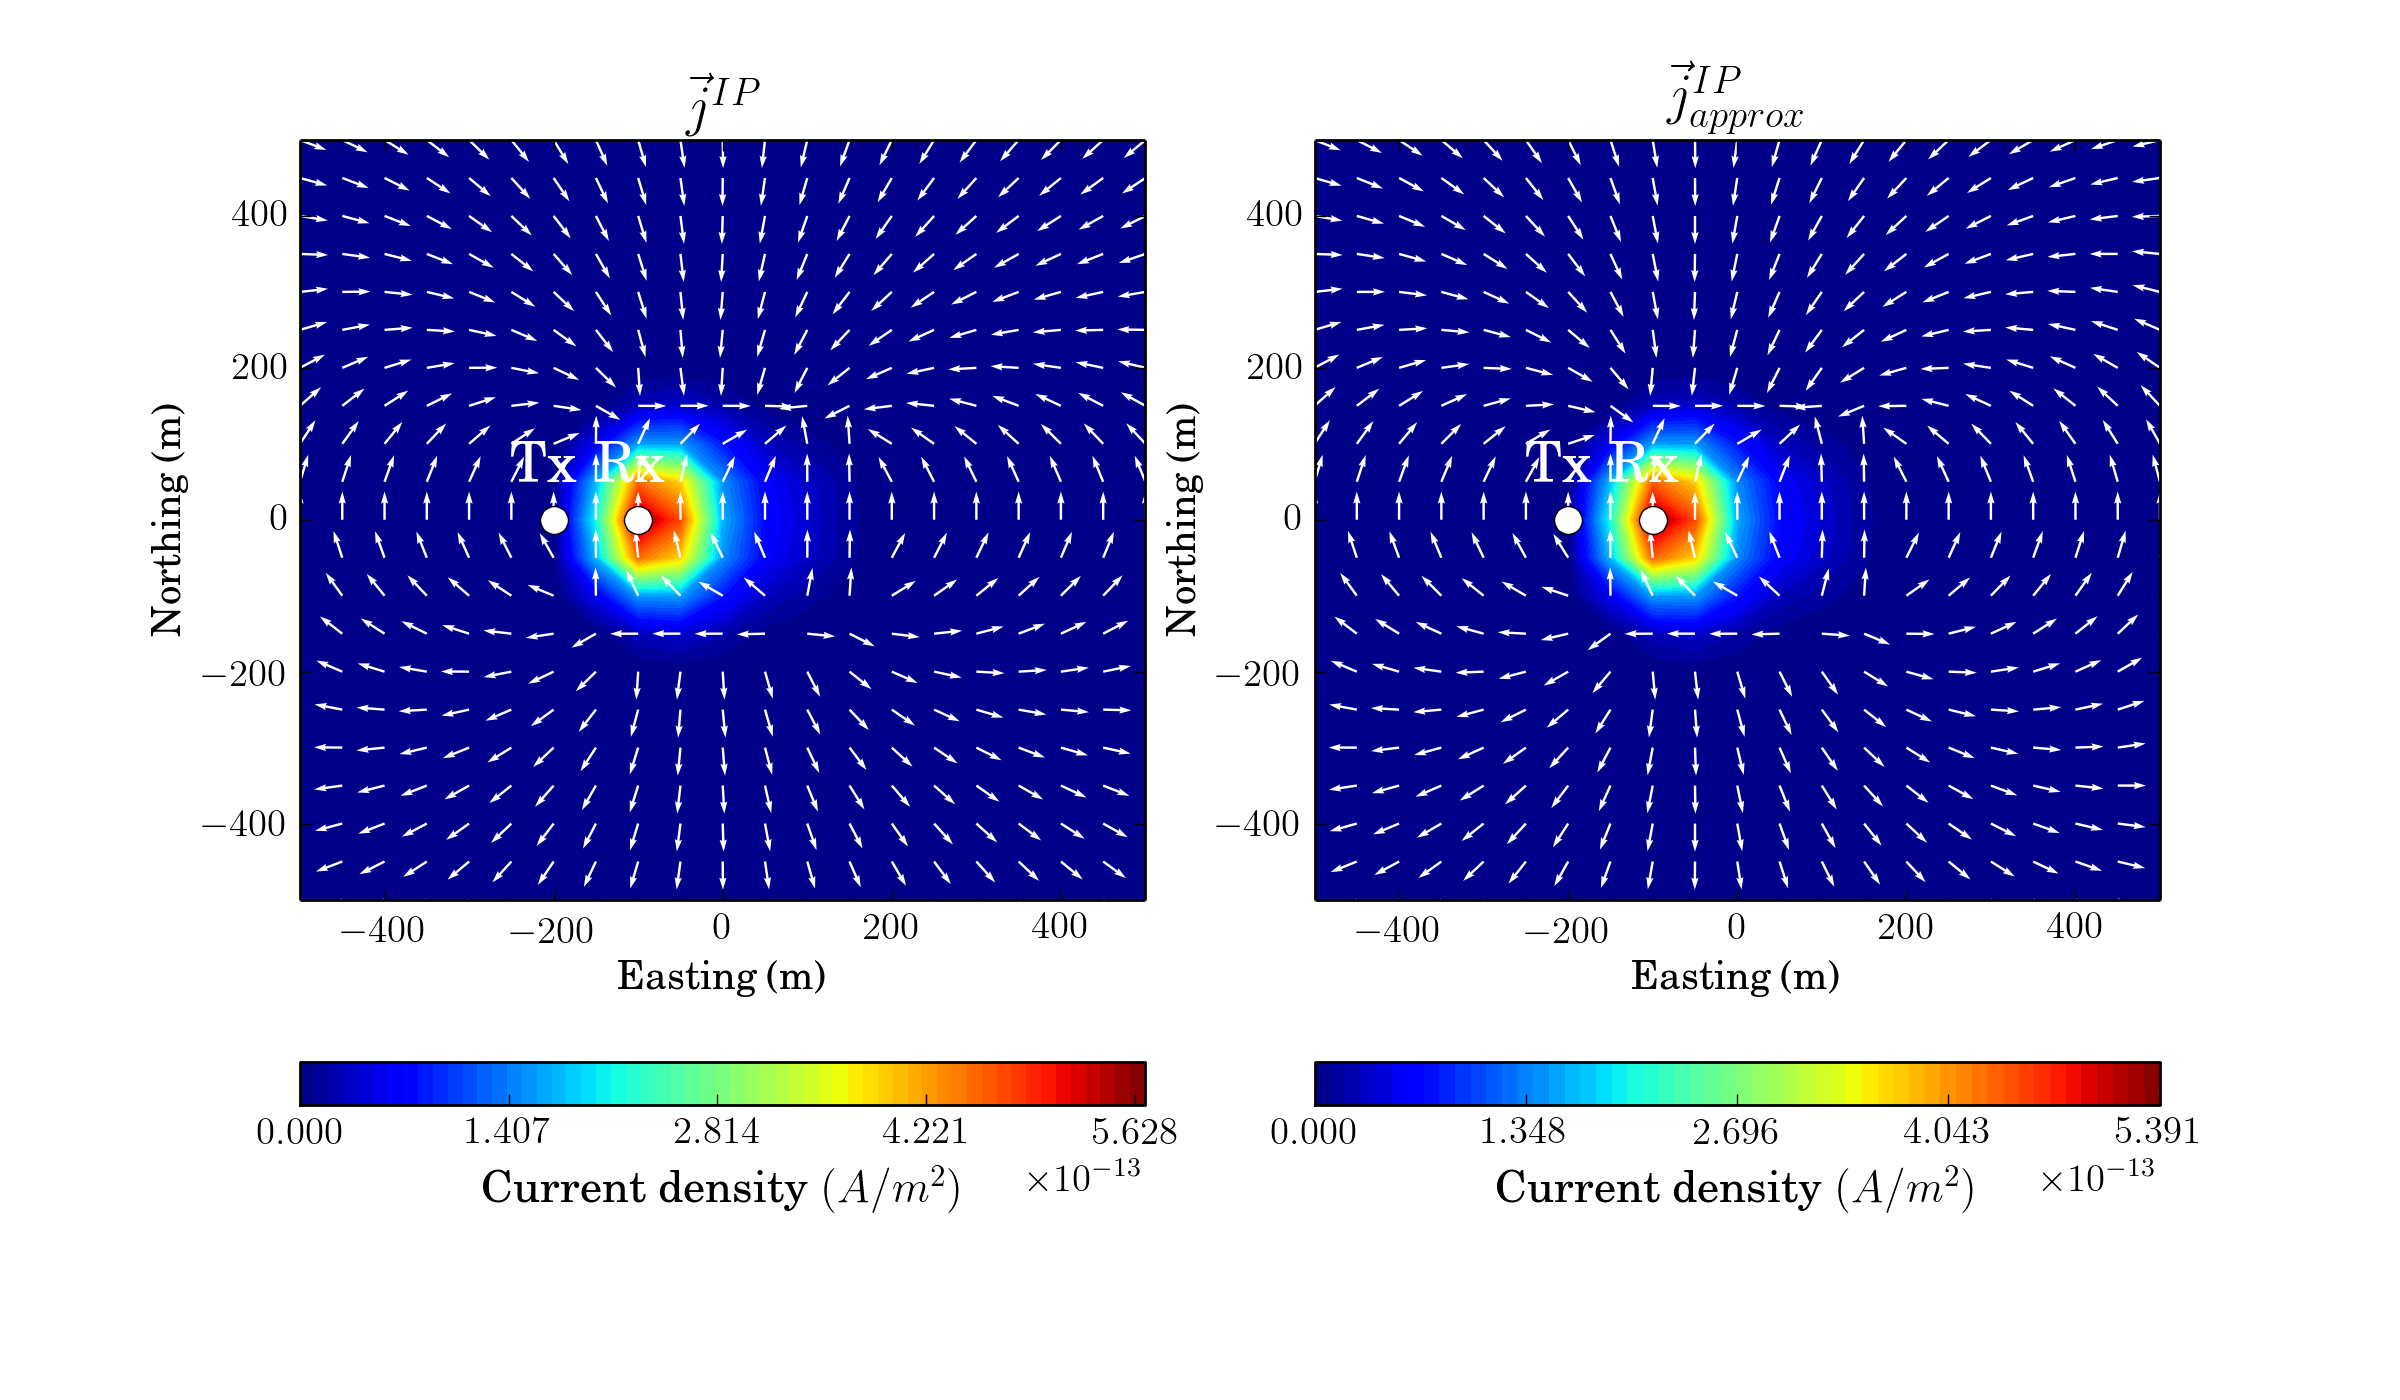
\includegraphics[height=0.4\textheight]{figures/synthetic/CurrentIP_case2_ch38.png} \\
  (b)
  \caption{(a) Time decaying curves of current densities at Rx location for conductive model. (a) $\j_y$ (black), $\j^F_y$ (blue) and $\j^{IP}_y$ (red). (b) $\j^{IP}_{y \ 1}$ (blue), $\j^{IP}_{y \ 2}$ (red) and $\j^{IP}_{y \ 3}$ (green).}
  \label{F: currentIP_case2_plan}
\end{figure}

\begin{figure}[htb]
  \centering
  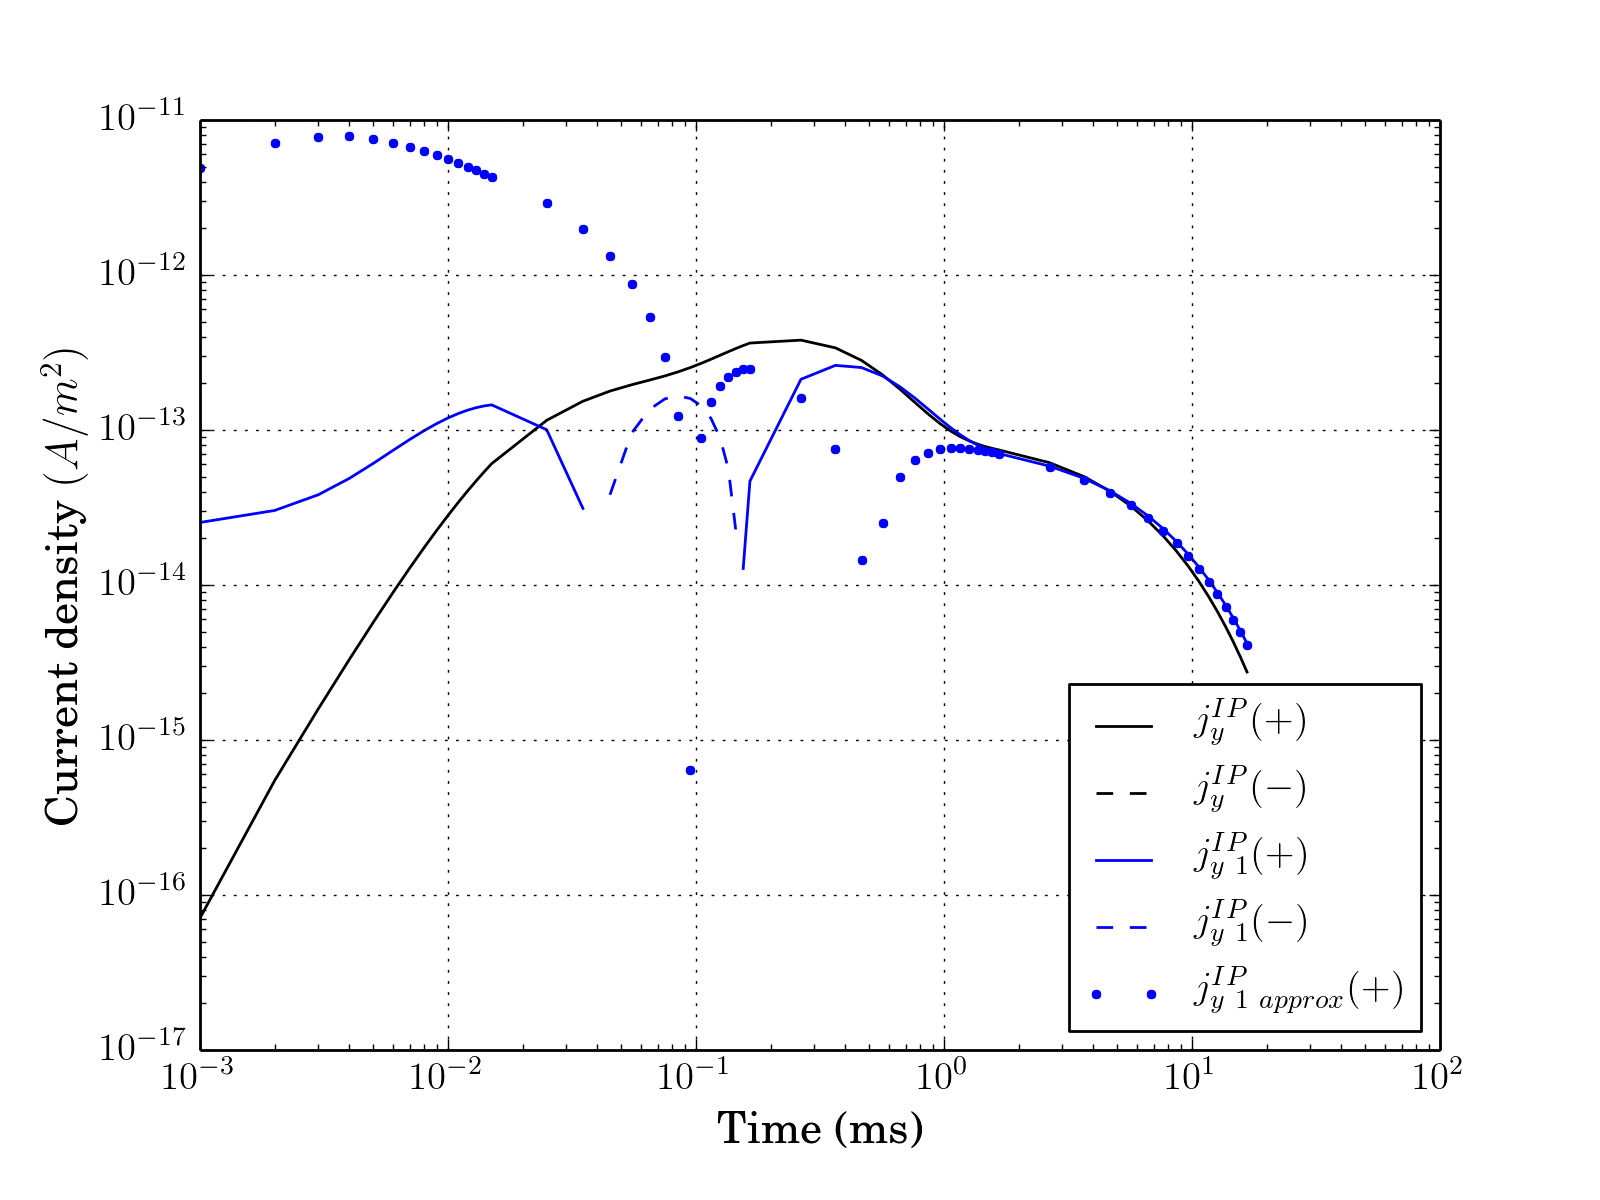
\includegraphics[height=0.4\textheight]{figures/synthetic/CurrentIP_decay_case2_1.png} \\
  \caption{Time decaying curves of $j_y^{IP}$ (black), $j_{y \ 1}^{IP}$ (blue) and $j_{y \ 1 \ approx}^{IP}$ (blue dots) at Rx location for conductive model. }
  \label{F: currentIP_case2_decay}
\end{figure}
\clearpage

\subsection{Linear inversion}
We apply linear inversion to restore 3D distribution of pseudo-chargeability at each time channels. In order to validate our inversion algorithm, we first generated synthetic IP data, $d^{IP}_{syn}$ for both canonical and conductive models using forward equation shown in equation (\ref{eq: BiotbIPdt_approx}). Floor noise of $0.01max(|\mathbf{d}^{obs}|)$ was added to $\dip_{syn}$, and we set this as our uncertainty ($\epsilon$). Here data type is $\frac{\partial b_z}{\partial t}$. We use same survey configuration that we used to compute $d^{IP}$ responses. As shown in Table 1, the number of data for each time channel is 121, since we have 121 stations. Our model parameter do not include air, thus the number of model parameters: 41$\times$41$\times$20=33620. Since our sensitivity function has higher values near the surface, we need to balance this biased sensitivity distribution. This has been carefully treated in magnetic inversion (CITE). Based on this, we use $\mathbf{w} = (\mathbf{z}+z_0)^{-1.5}$ with $z_0$=0 for model weighting shown in equation (\ref{eq: weight_mat}). Here $\mathbf{z}$ is discretized depth for all model parameters, $z_0$ indicates the depth of the earth surface. Other inversion parameters are shown in Table 1. A constant, related to initial $\beta$, $r_{\beta}$ is set to 1. To generate sensitivity matrix shown in equation (\ref{eq: dbIPdt_linear}), we used true background conductivity model for both cases. Same Cole-Cole parameters are used ($\eta$=0.2, $\tau$=0.005 and $c$=1), and for $\peta$ we used $\peta^{I}$, which was shown in equation (\ref{eq: intrinsic_peta}) when $c$=1.

\begin{table}[ht]
\caption{Parameters used in Projected Gauss Newton inversion.} % title of Table
\centering % used for centering table
\begin{tabular}{c c} % centered columns (4 columns)
\hline\hline %inserts double horizontal lines
Inversion parameters & Value \\
[0.1ex] % inserts table
\hline
The number of data &    11$\times$11=121 \\
The number of models &  41$\times$41$\times$20=33620 \\
$\alpha_s$ &  $10^{-5}$\\
$\alpha_x$ &  1\\
$\alpha_y$ &  1\\
$\alpha_z$ &  1\\
Initial $\beta$ &  $r_{\beta}\frac{\mathbf{x}^T\mathbf{J}^T\mathbf{J}\mathbf{x}}{\mathbf{x}^T\mathbf{W}_m^T\mathbf{W}_m\mathbf{x}}$\\
Decrease rate of $\beta$ &  0.5\\
The number of $\beta$ iteration & 2\\
$\mathbf{m}_{ref}$ & $10^{-10}$ \\
Uncertainty & $\epsilon$=$0.01$max($|\mathbf{d}^{obs}|$) \\
Bound constraint & $\mathbf{m} > 0$\\
\hline %inserts single line
\end{tabular}
\label{table:1} % is used to refer this table in the text
\end{table}

Linear inversions are applied $d^{IP}_{syn}$ data at t=4.7 ms so that corresponding $\peta^I$ value for IP body is 8.52. In Figure ~\ref{F: Peta_dipsyn_ch38}a and b, we presented inverted peudo-chargeablity models for both canonical and conductive models, respectively. To show reliability of our inversion, observed and predicted data for both canonical and conductive model were shown in Figure ~\ref{F: ObsPred_syn_ch38}a and b, respectively. Observed and predicted data for both cases show reasonable matches. Also, both inversions were reached to th target misfit. In both cases, geometry of IP body was well imaged in right location, whereas estimated $\peta$ for canonical model shows somewhat blurred image compared to that for conductive model. Recovered $\peta$ values in the IP body for both cases were $~$1.5 and $~$4.4, whereas true $\peta$ value for the IP body was 8.72. As Figure ~\ref{F: ObsPred_syn_ch38}a and b, $d^{IP}_{syn}$ for canonical model shows broader distribution than that for conductive model, which may explain different magnitude of restored $\peta$ for both cases. These observations of recovered $\peta$ for both cases shows that recovered model from conductive model can have bigger magnitude compared to canonical model. In addition, by comparing $d^{IP}_{syn}$ shown in the left panel of Figure ~\ref{F: ObsPred_syn_ch38}a and b with true $\dip$ data shown in the right panels of Figures ~\ref{F: EMIPresp2_case1}b and ~\ref{F: EMIPresp2_case2}b, we recognize that their geometric distribution for both cases are analogous, whereas their absolute values are different. This suggest the reliability of our linearization approach.

\begin{figure}[htb]
  \centering
  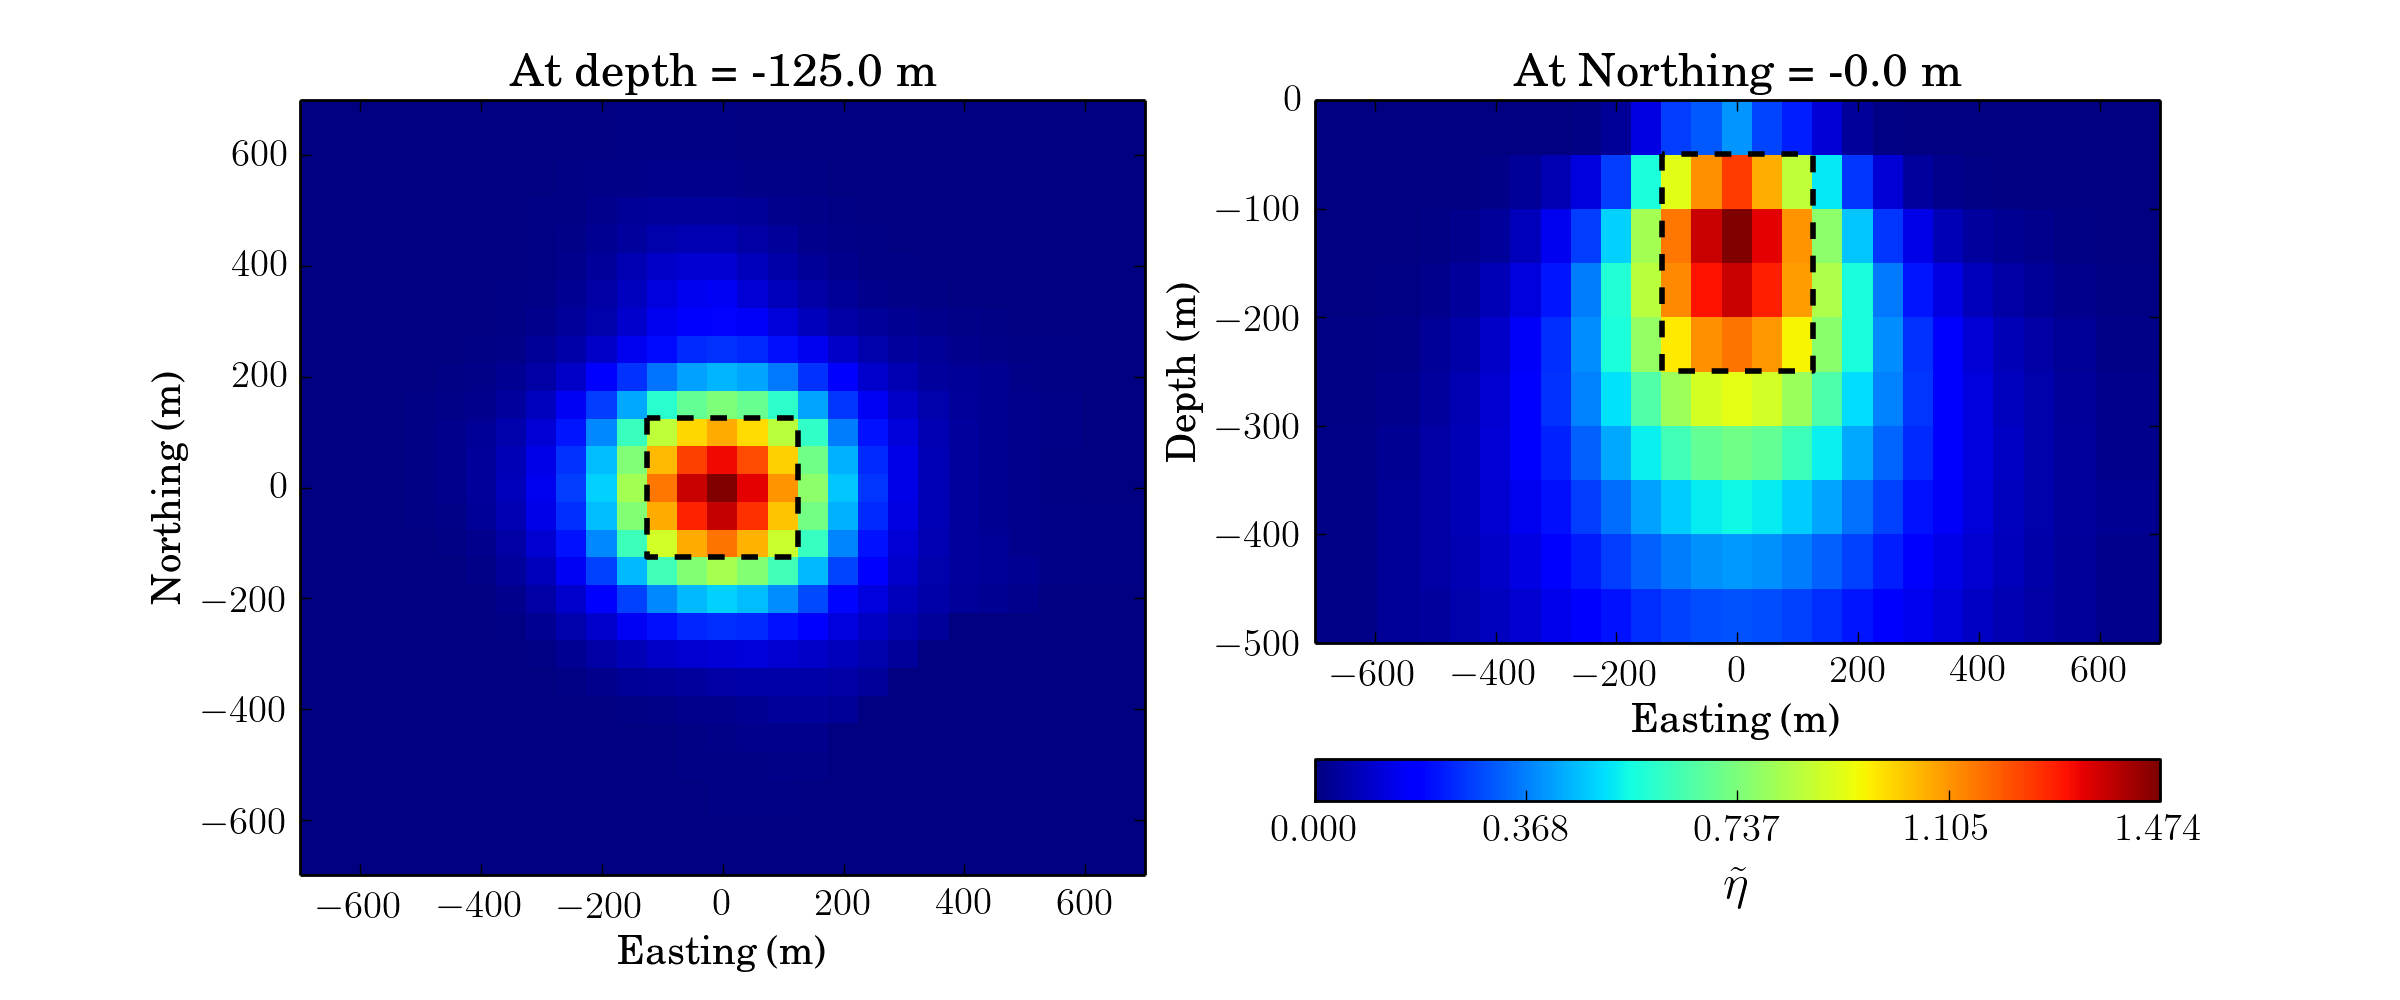
\includegraphics[width=\textwidth]{figures/synthetic/PetaCase1_syn_ch38.png}\\
  (a)
  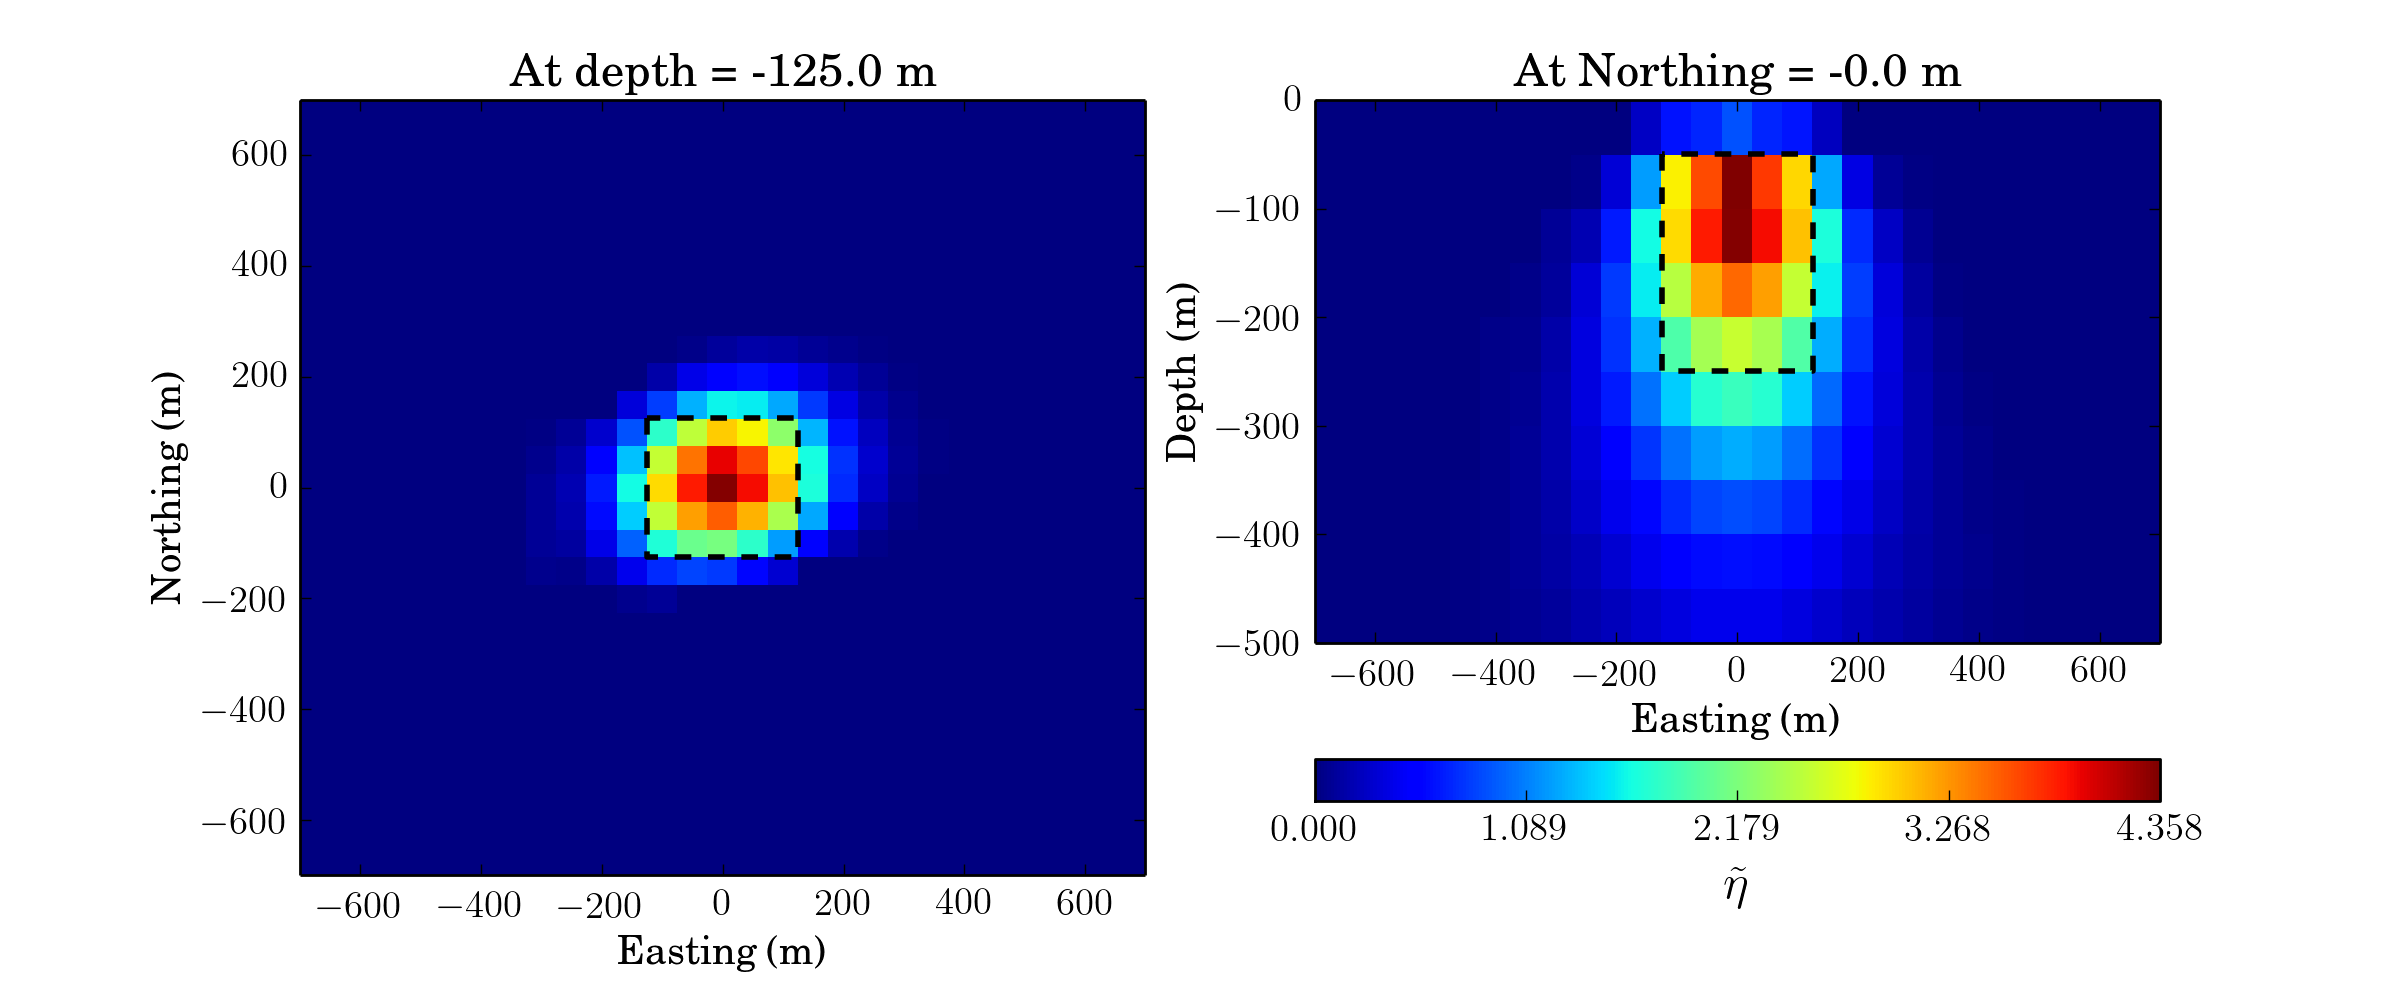
\includegraphics[width=\textwidth]{figures/synthetic/PetaCase2_syn_ch38.png}\\
  (b)
  \caption{Slices of estimated $\peta$ distributions at $t = $ 4.7 ms by inverting $d^{IP}_{syn}$. (a) Canonical model. (b)  Conductive model. Left and right panel show plan and section view at -125 m depth and 0 m northing. Black dashed lines outline IP body. }
  \label{F: Peta_dipsyn_ch38}
\end{figure}

\begin{figure}[htb]
  \centering
  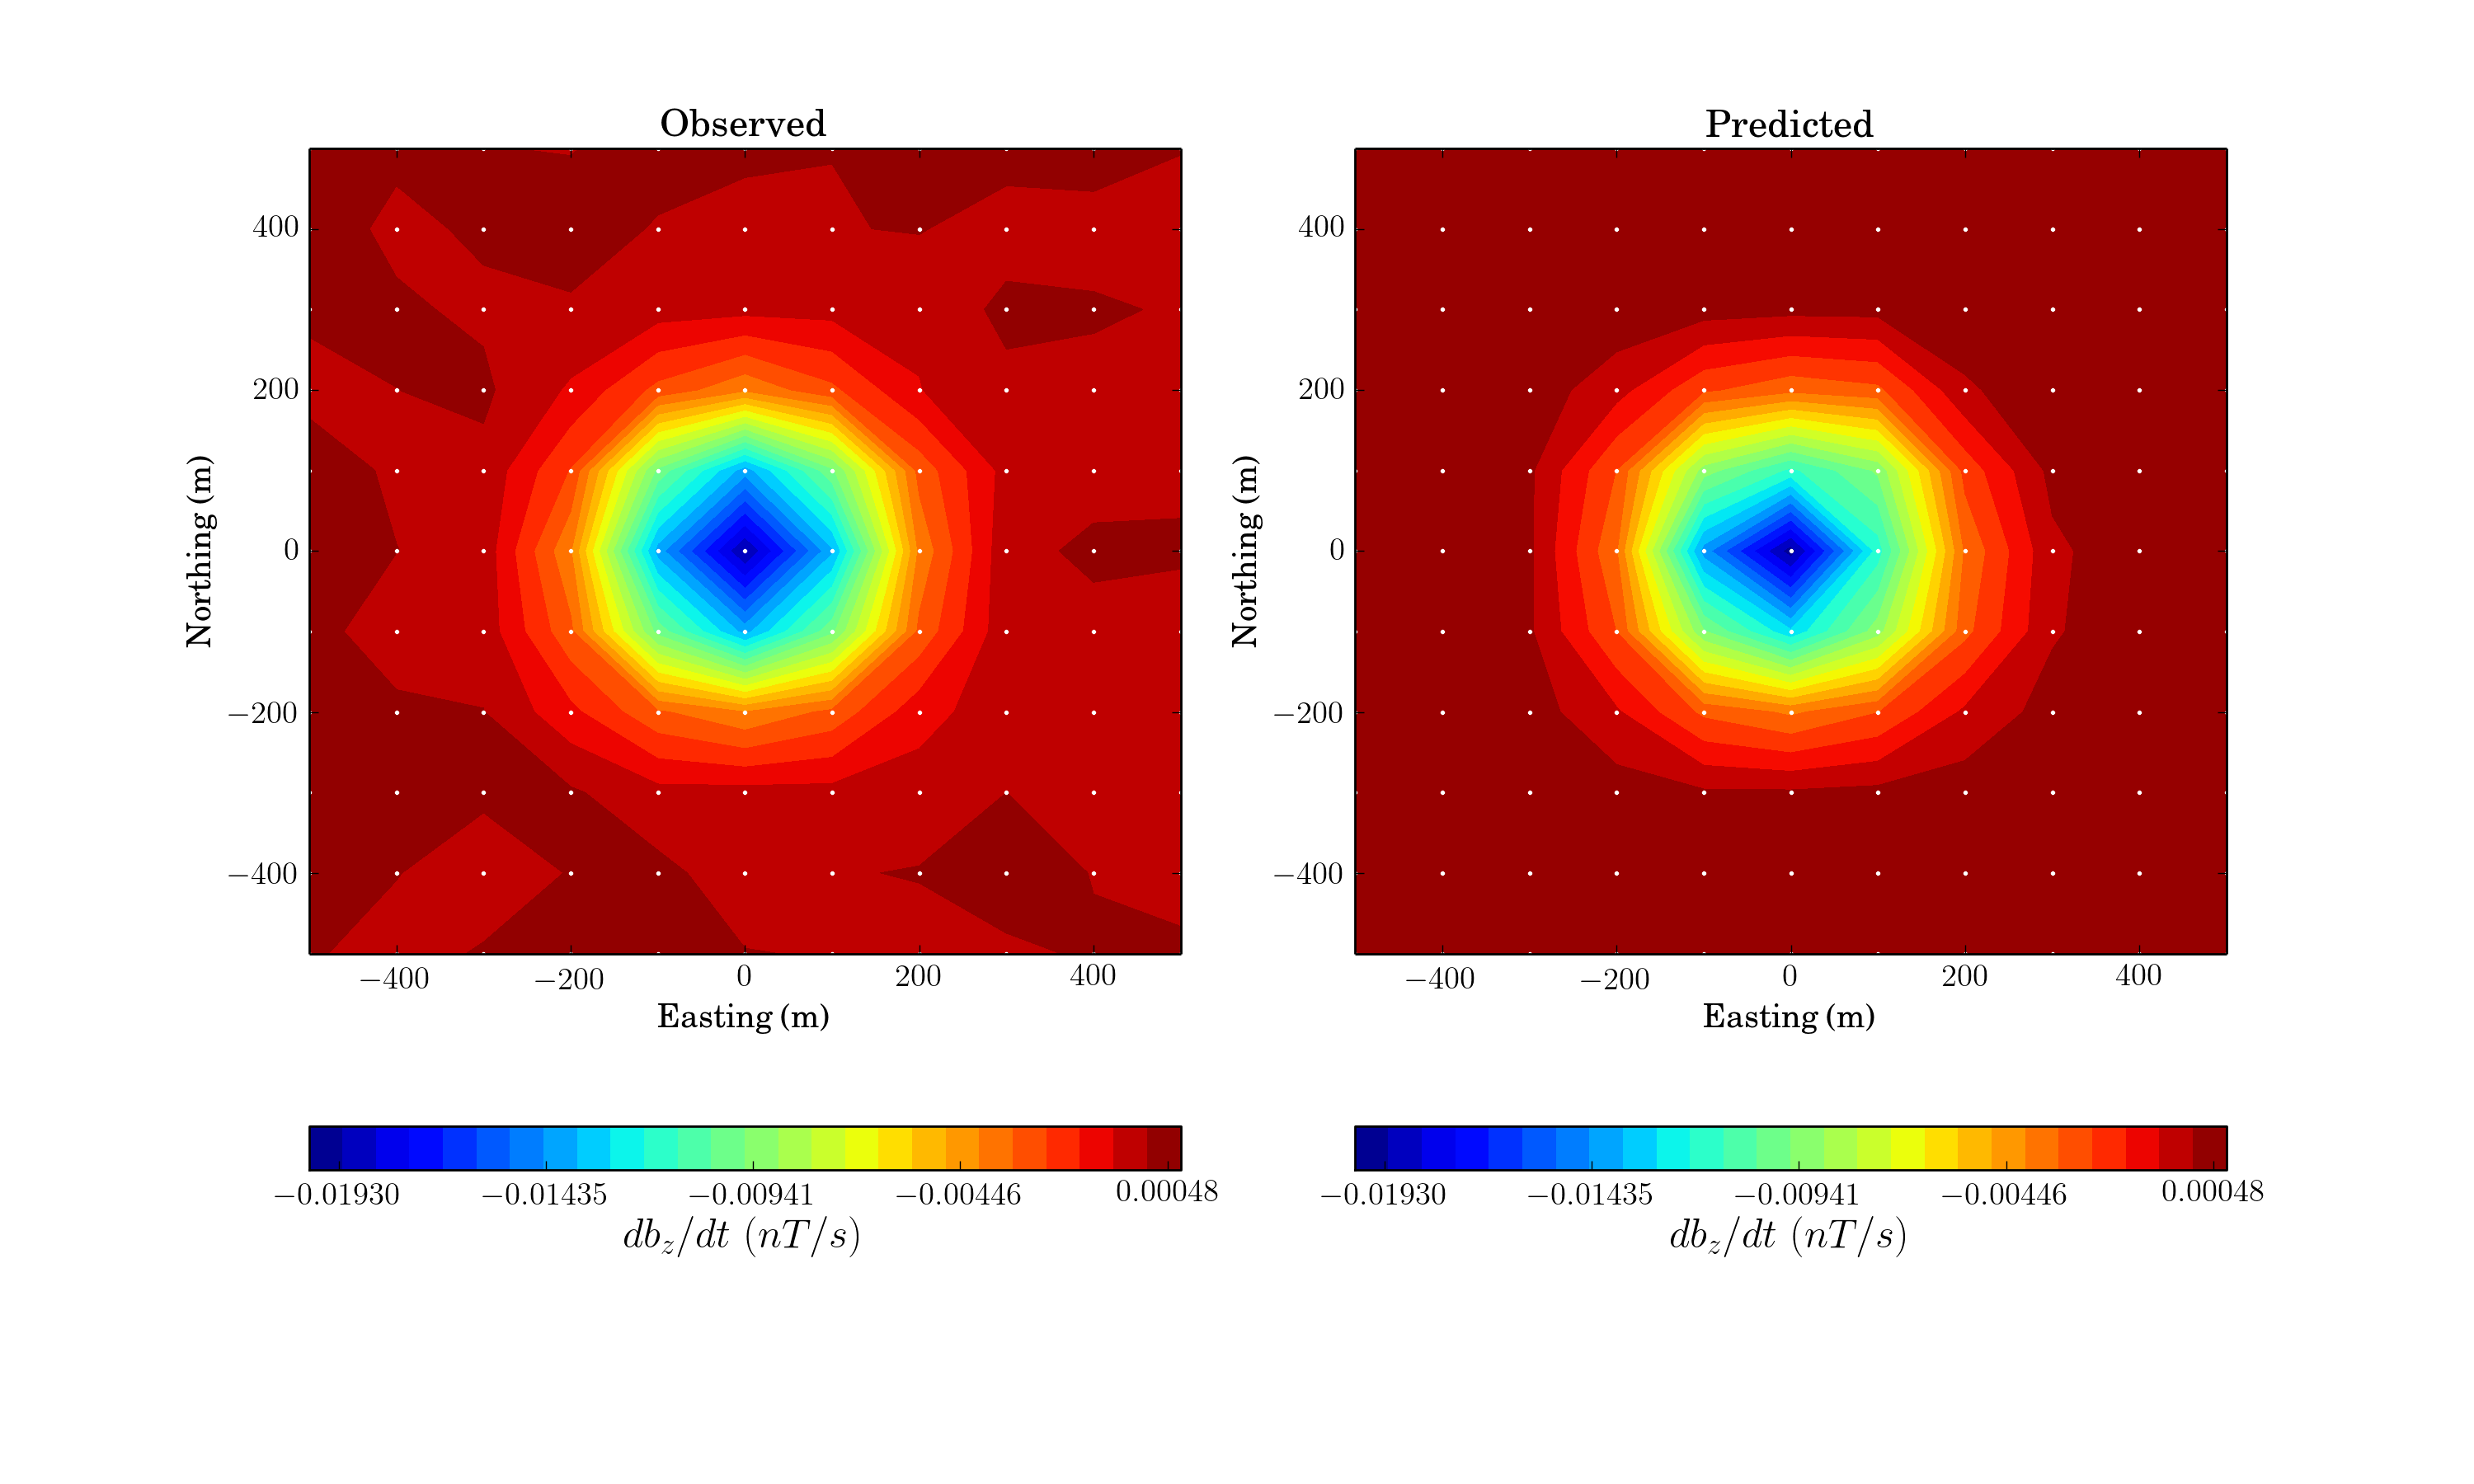
\includegraphics[width=\textwidth]{figures/synthetic/ObsPred_syn_ch38_case1.png}\\
  (a)
  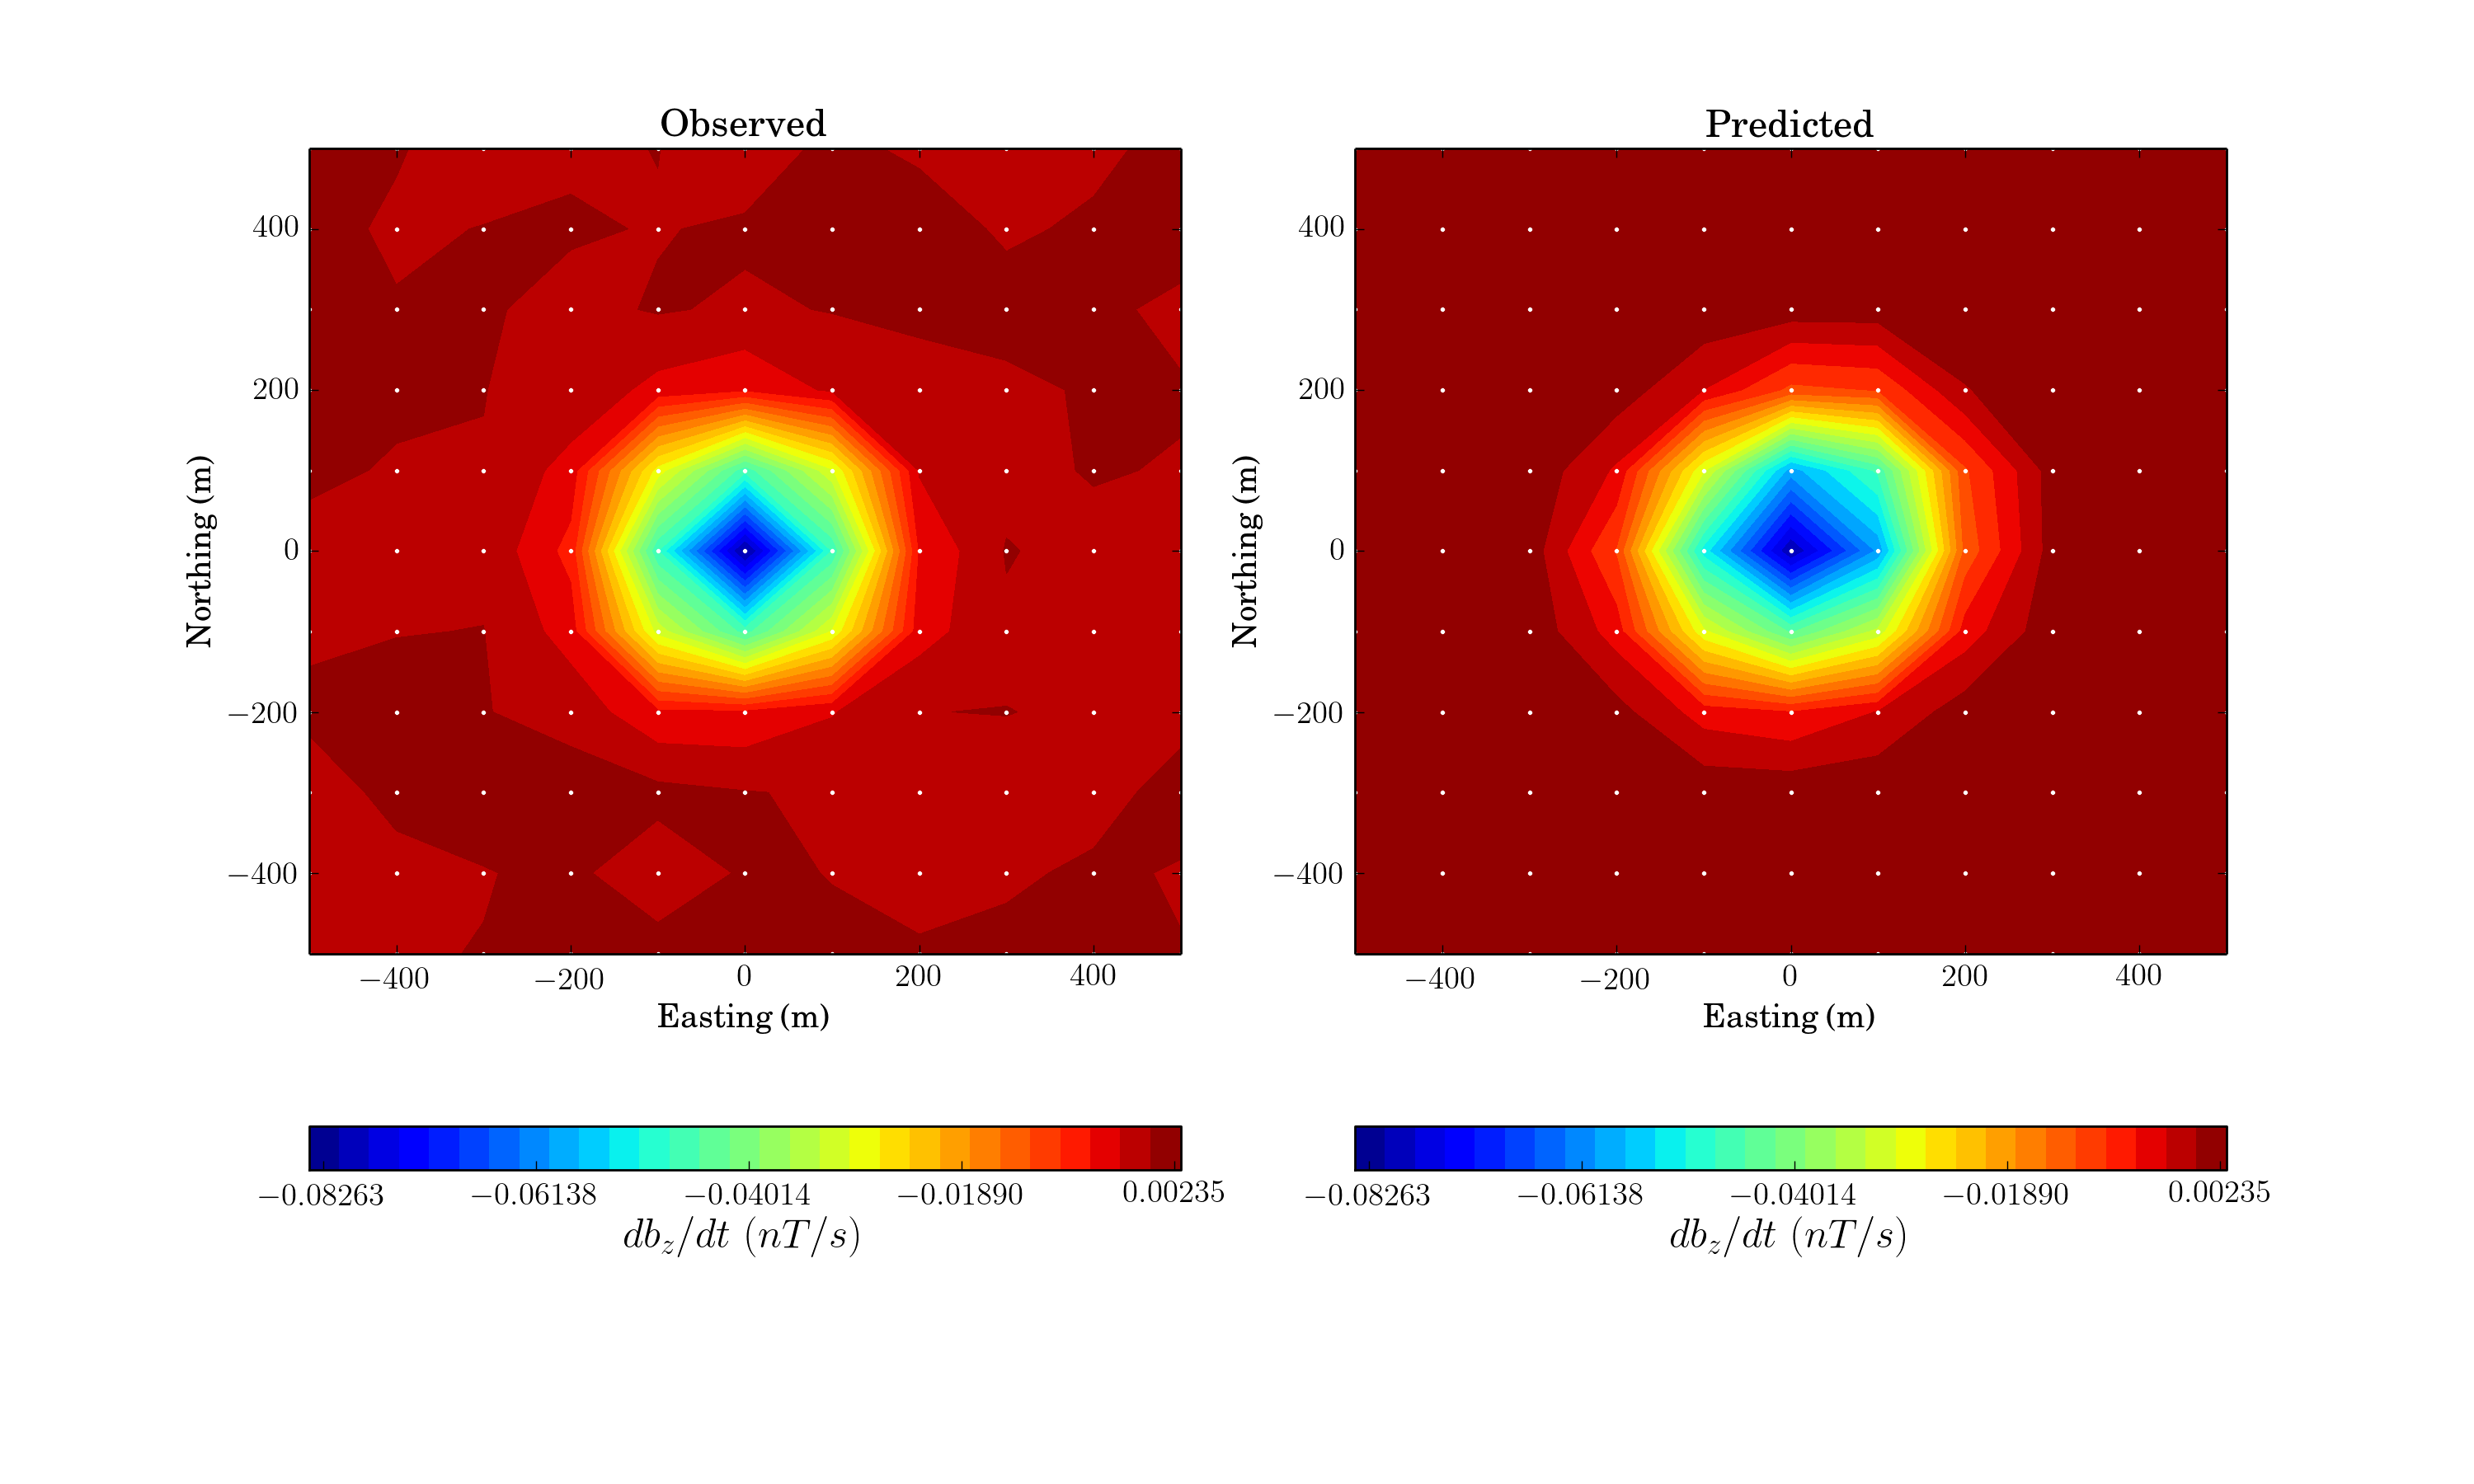
\includegraphics[width=\textwidth]{figures/synthetic/ObsPred_syn_ch38_case2.png}\\
  (b)
  \caption{Slices of estimated $\peta$ distributions at $t = $ 4.7 ms by inverting $d^{IP}_{syn}$. (a) Canonical model. (b)  Conductive model. Left and right panel show plan and section view at -125 m depth and 0 m northing. Black dashed lines outline IP body. }
  \label{F: ObsPred_syn_ch38}
\end{figure}

On the other hand, we consider true $d^{IP}$ data at t=4.7 ms, which was generated by subtracting $d^{F}$ from $d$ as shown in the right panels of Figures ~\ref{F: EMIPresp2_case1}b and ~\ref{F: EMIPresp2_case2}b. Since $\peta$ is convoluted property of electric field and $\peta^{I}$, we need to evaluate restored $\peta$ can suggest meaningful information about the embedded IP body. Same survey configuration and inversion parameters were used as above examples for $d^{IP}_{syn}$ except $r_{\beta}$=0.1. In Figure ~\ref{F: Peta_dip_ch38}a and b, we presented restored pseudo-chargeability models for both canonical and conductive models, respectively. Both inversions for canonical and conductive models were reached to the target misfit. Recovered $\peta$ models for both cases show reasonable geometry of IP body, whereas absolute magnitude of them are quite different from $\peta^{I}$. However, $\peta$ is convoluted property of $\e(t)$ and $\peta^{I}$ so that absolute value of restored $\peta$ does not have meaningful information. Therefore, restored $\peta$ can suggest geometry of IP body in the earth. Similar patterns from recovered $\peta$ models of $\dip_{syn}$ can be observed here: restored model from canonical model show broader distribution and smaller magnitude of $\peta$ than that from conductive model. Accordingly, identification of relative strength of $\peta^I$ for different IP bodies might depend on background conductivity model. In addition, to investigate effect of wrong background model, we invert $d^{IP}$ data for conductive model using sensitivity matrix generated for canonical model. Restored $\peta$ distribution is shown in Figure ~\ref{F: Peta_case2_wrong_ch38} and it is almost same as Figure ~\ref{F: Peta_dip_ch38}b, which used correct sensitivity matrix. This shows the robustness of our inversion to background conductivity model. However, note that this effect in EM decoupling process can be more significant.

\begin{figure}[htb]
  \centering
  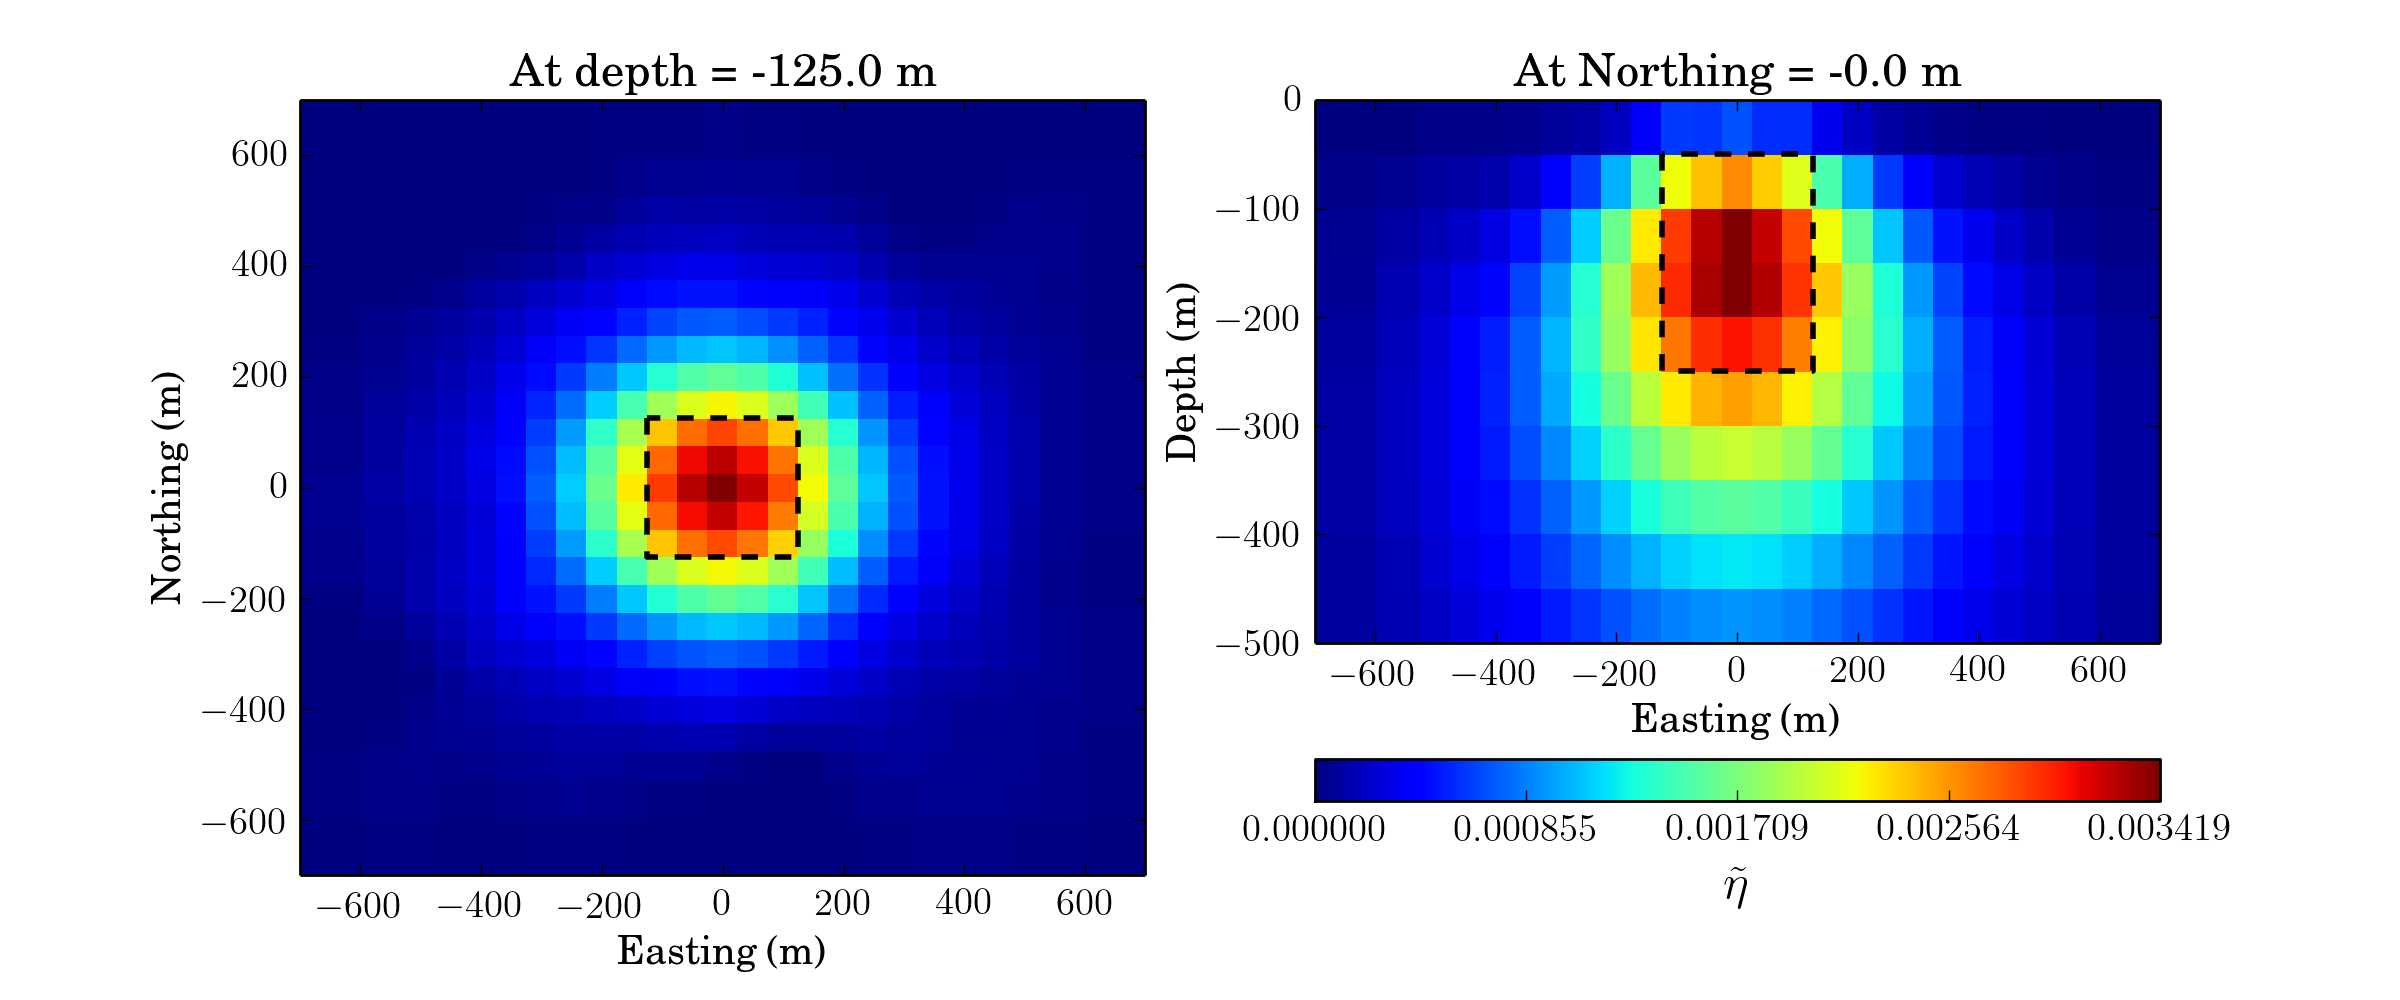
\includegraphics[width=\textwidth]{figures/synthetic/PetaCase1_true_ch38.png}\\
  (a)
  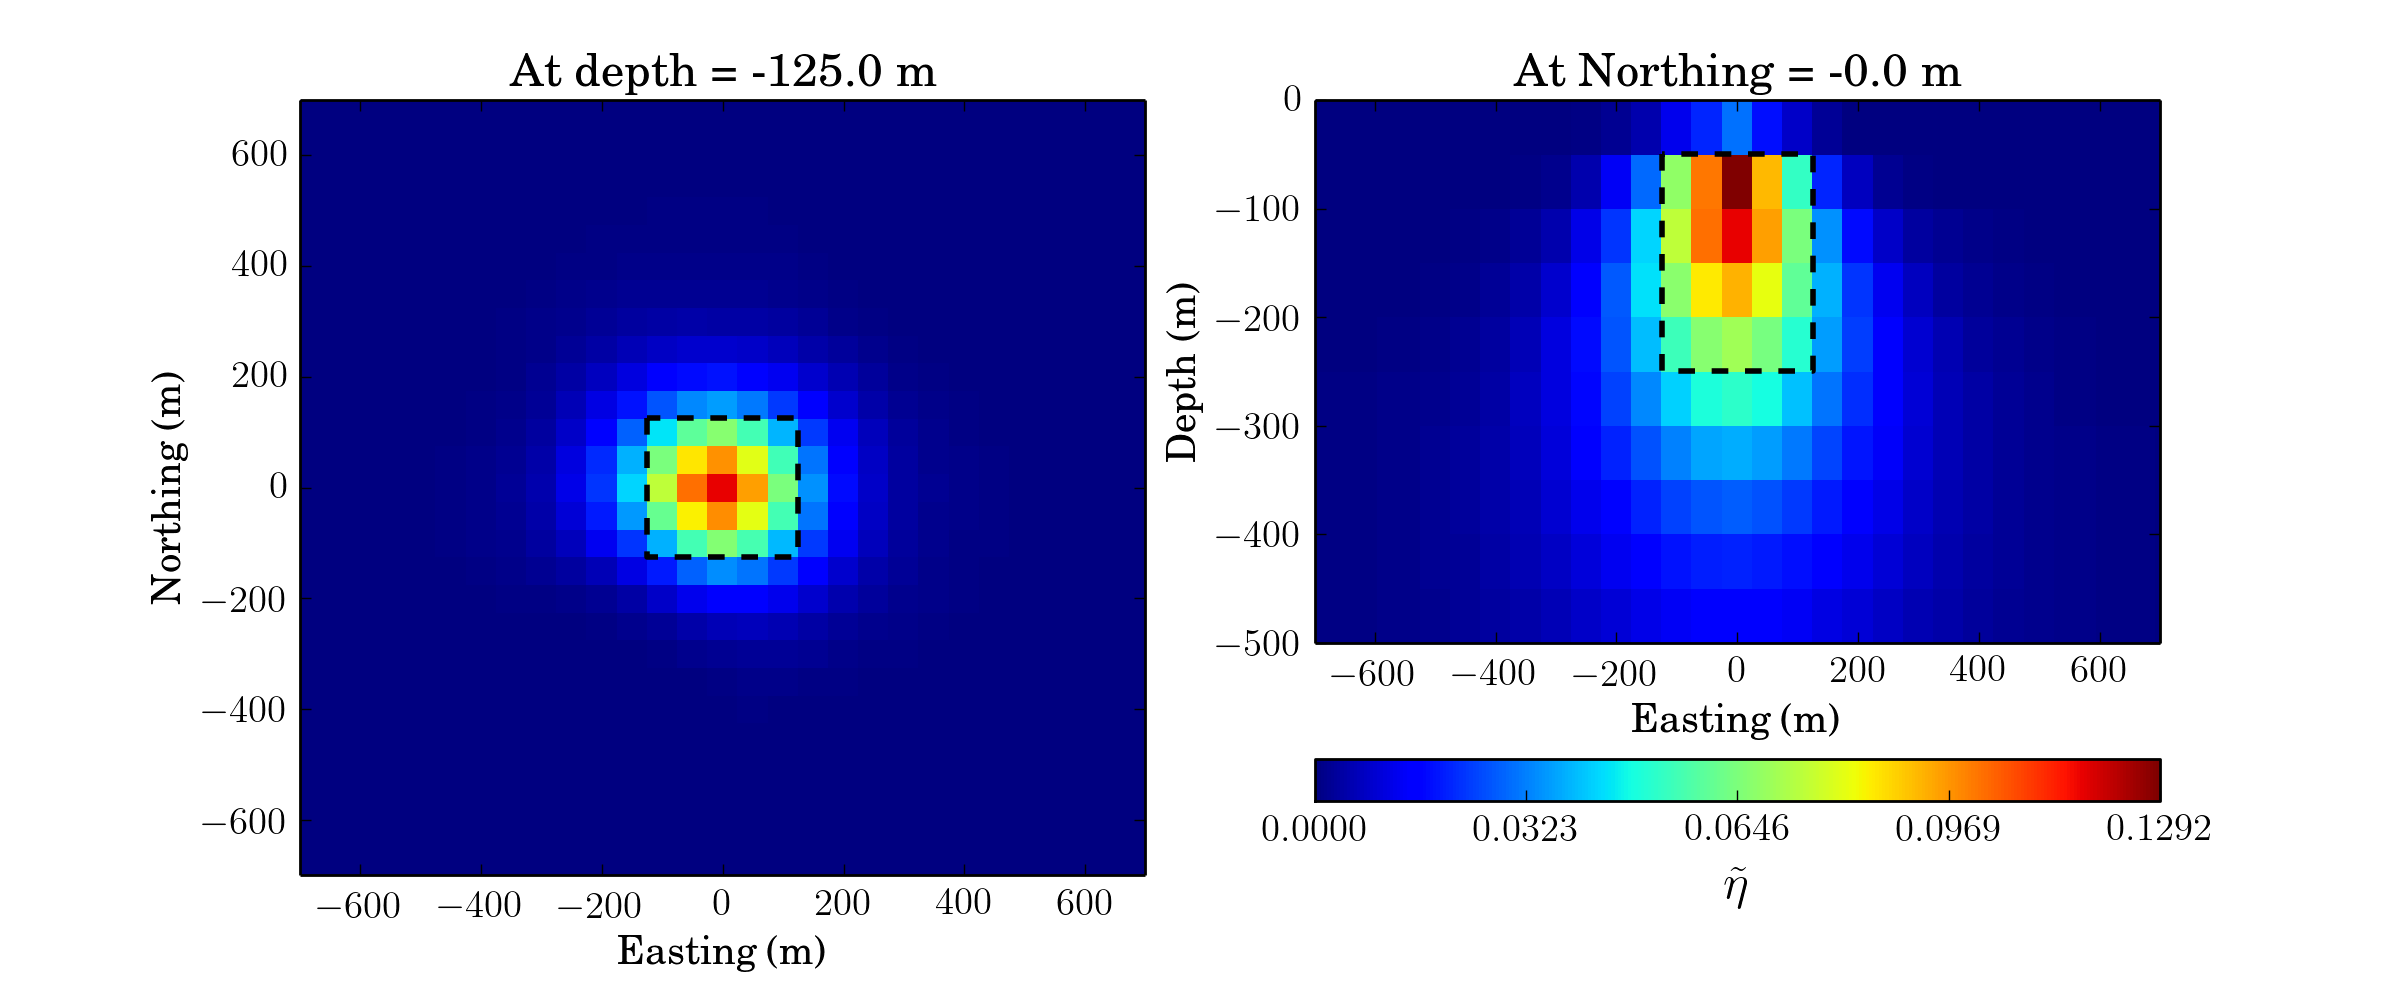
\includegraphics[width=\textwidth]{figures/synthetic/PetaCase2_true_ch38.png}\\
  (b)
  \caption{Slices of estimated $\peta$ distributions at $t = $ 4.7 ms  by inverting $d^{IP}$. (a) Canonical model. (b)  Conductive model.. Left and right panel show plan and section view at -125 m depth and 0 m northing. }
  \label{F: Peta_dip_ch38}
\end{figure}

\begin{figure}[htb]
  \centering
  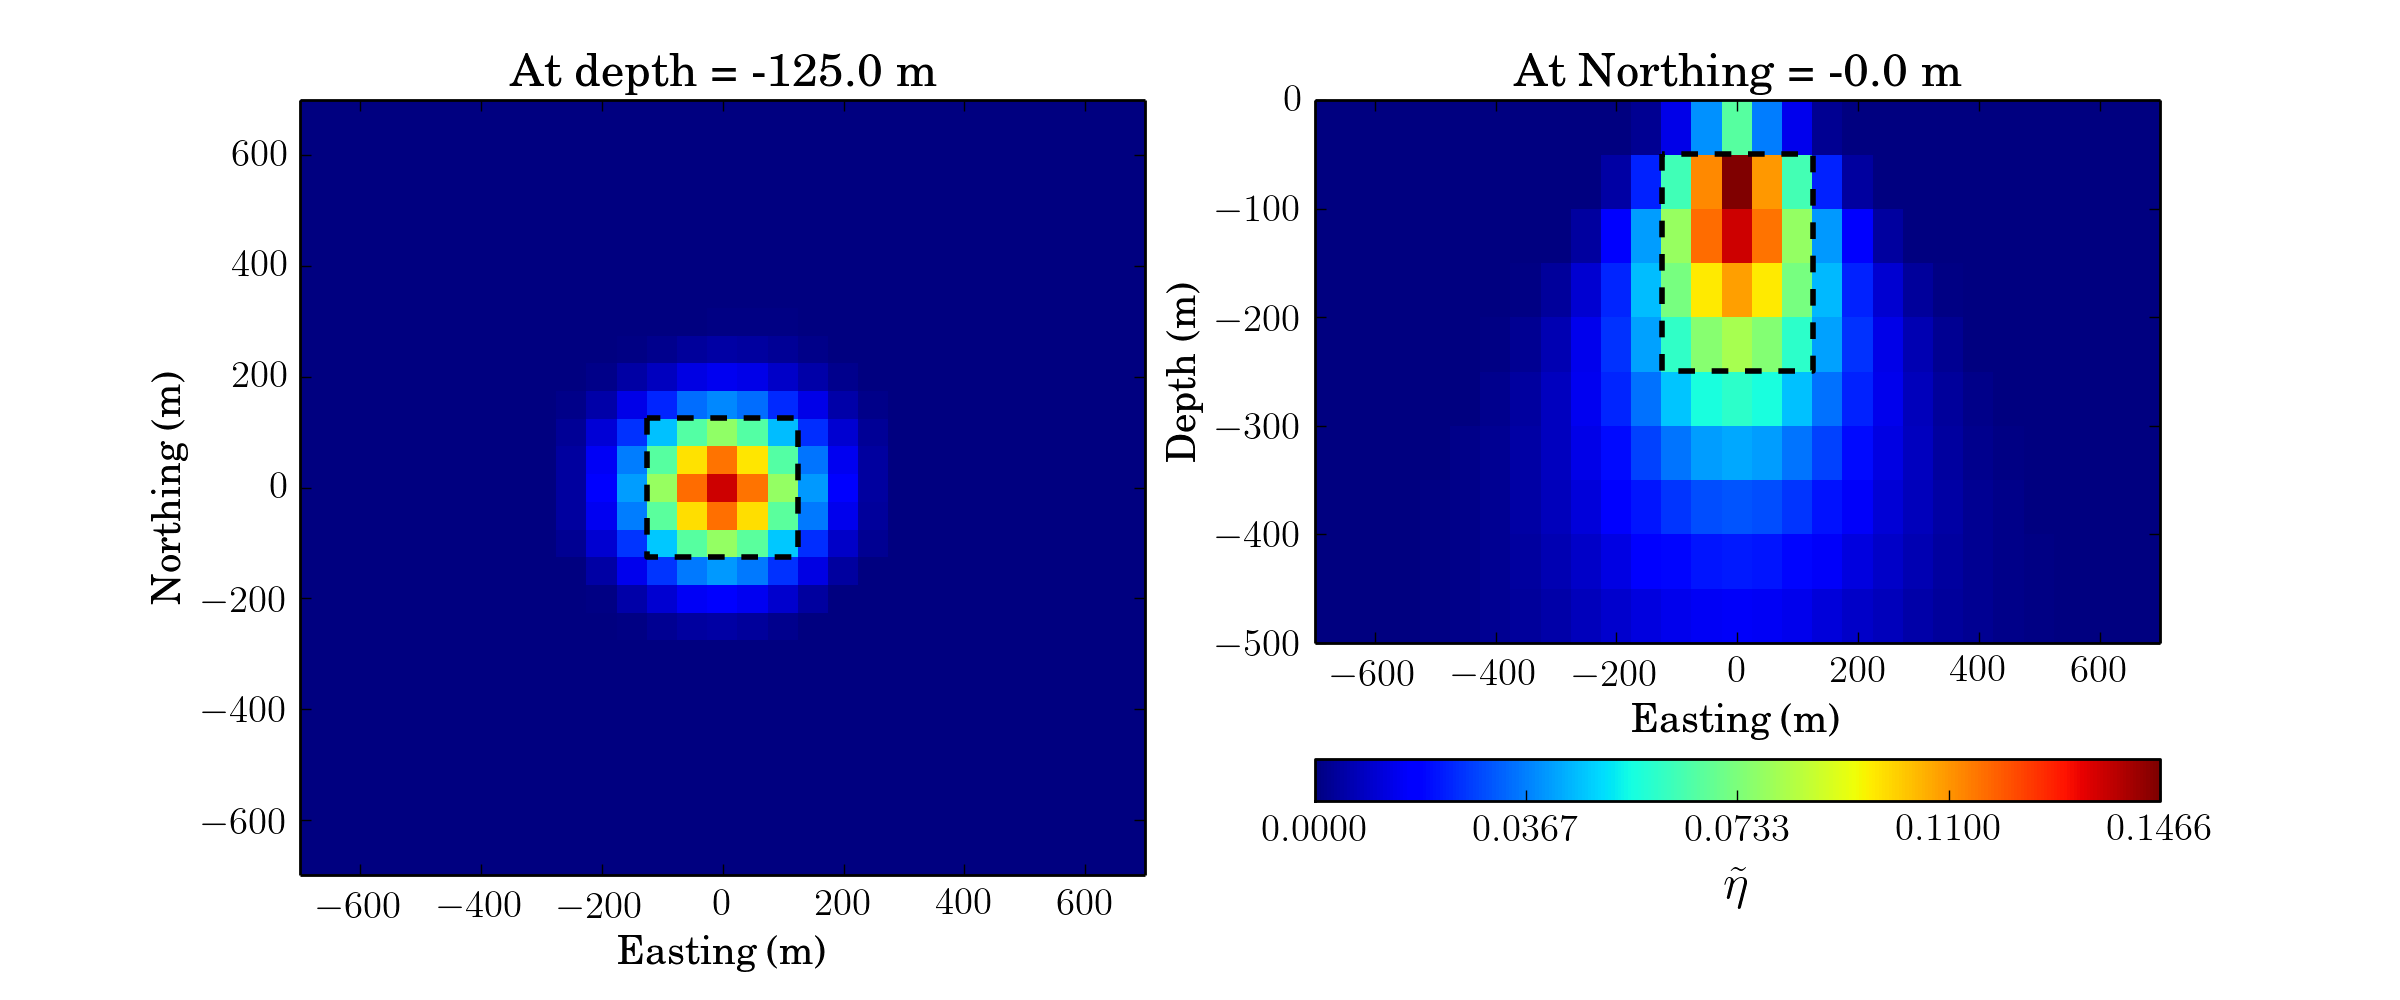
\includegraphics[width=\textwidth]{figures/synthetic/PetaCase2_wrong_ch38.png}
  \caption{Slices of estimated $\peta$ distributions at $t = $ 4.7 ms for conductive model with incorrect background conductivity model. Left and right panel show plan and section view at -125 m depth and 0 m northing. }
  \label{F: Peta_case2_wrong_ch38}
\end{figure}

Finally, using same survey and inversion set-ups, we inverted 14 time channels of $\d^{IP}$ ranging from 1 to 10 ms for both cases. We presented time decaying curves of restored $\peta$ models at (0, 0, -125) for both cases in Figure ~\ref{F: Peta_Center}a and b. Since we already recognized absolute value of the estimated pseudo-chargeability, $\peta_{est}$ is not meaningful, significant magnitude difference between $\peta^{est}$ and $\peta^I$ makes sense. However, we identify slope of $\peta^{est}$ and $\peta^I$ looks similar in later time channels (2-10 ms) for both cases. Taking log to equation (\ref{eq: intrinsic_peta}) yields
\begin{equation}
    log(\peta^{I}) = log(\frac{\eta}{(1-\eta)\tau}) - \frac{1}{(1-\eta)\tau}t,
\end{equation}
which can be considered as linear equation. To estimate slope of the above equation, $- \frac{1}{(1-\eta)\tau}$, we fit active set of the recovered pseudo chageability, $\peta^{est}_{active}$ ranging from 2.5 ms to 10 ms. Estimated slopes for canonical and conductive models are -203 and -218 when the true slope is -250. Corresponding relative errors are 12 and 13$\%$. This is promising result, which suggests potential of restoring intrinsic Cole-Cole parameters from recovered $\peta$ model at each time channel.

\begin{figure}[htb]
  \centering
  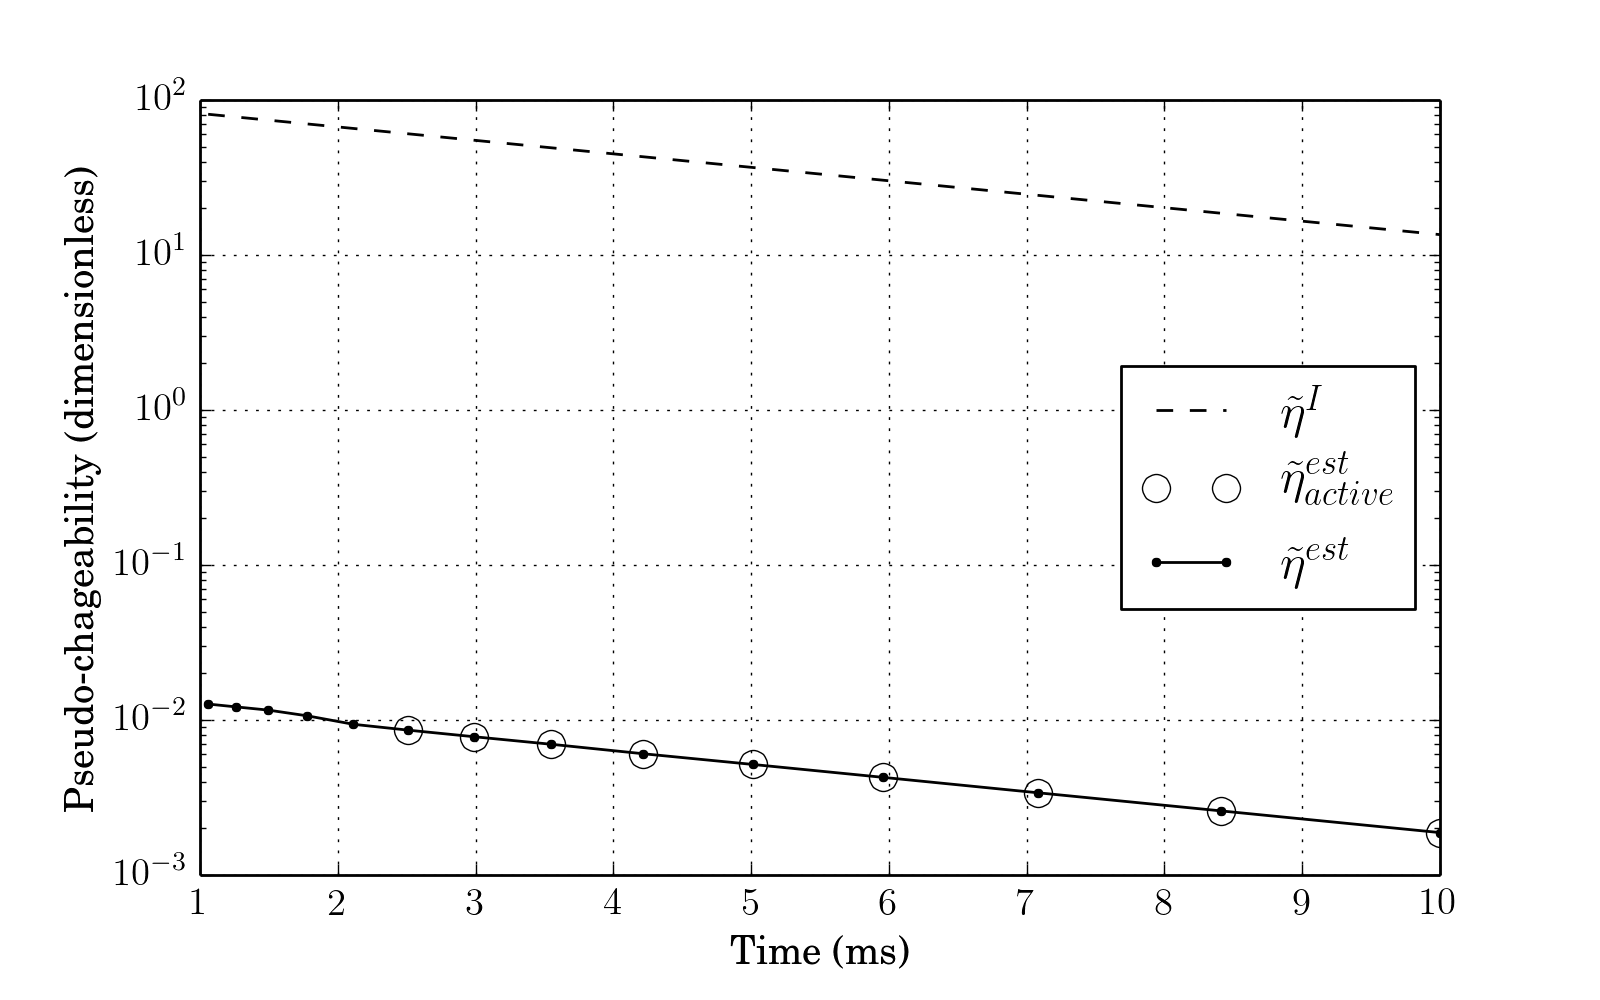
\includegraphics[width=0.8\textwidth]{figures/synthetic/PetaCase1_center.png} \\(a)\\
  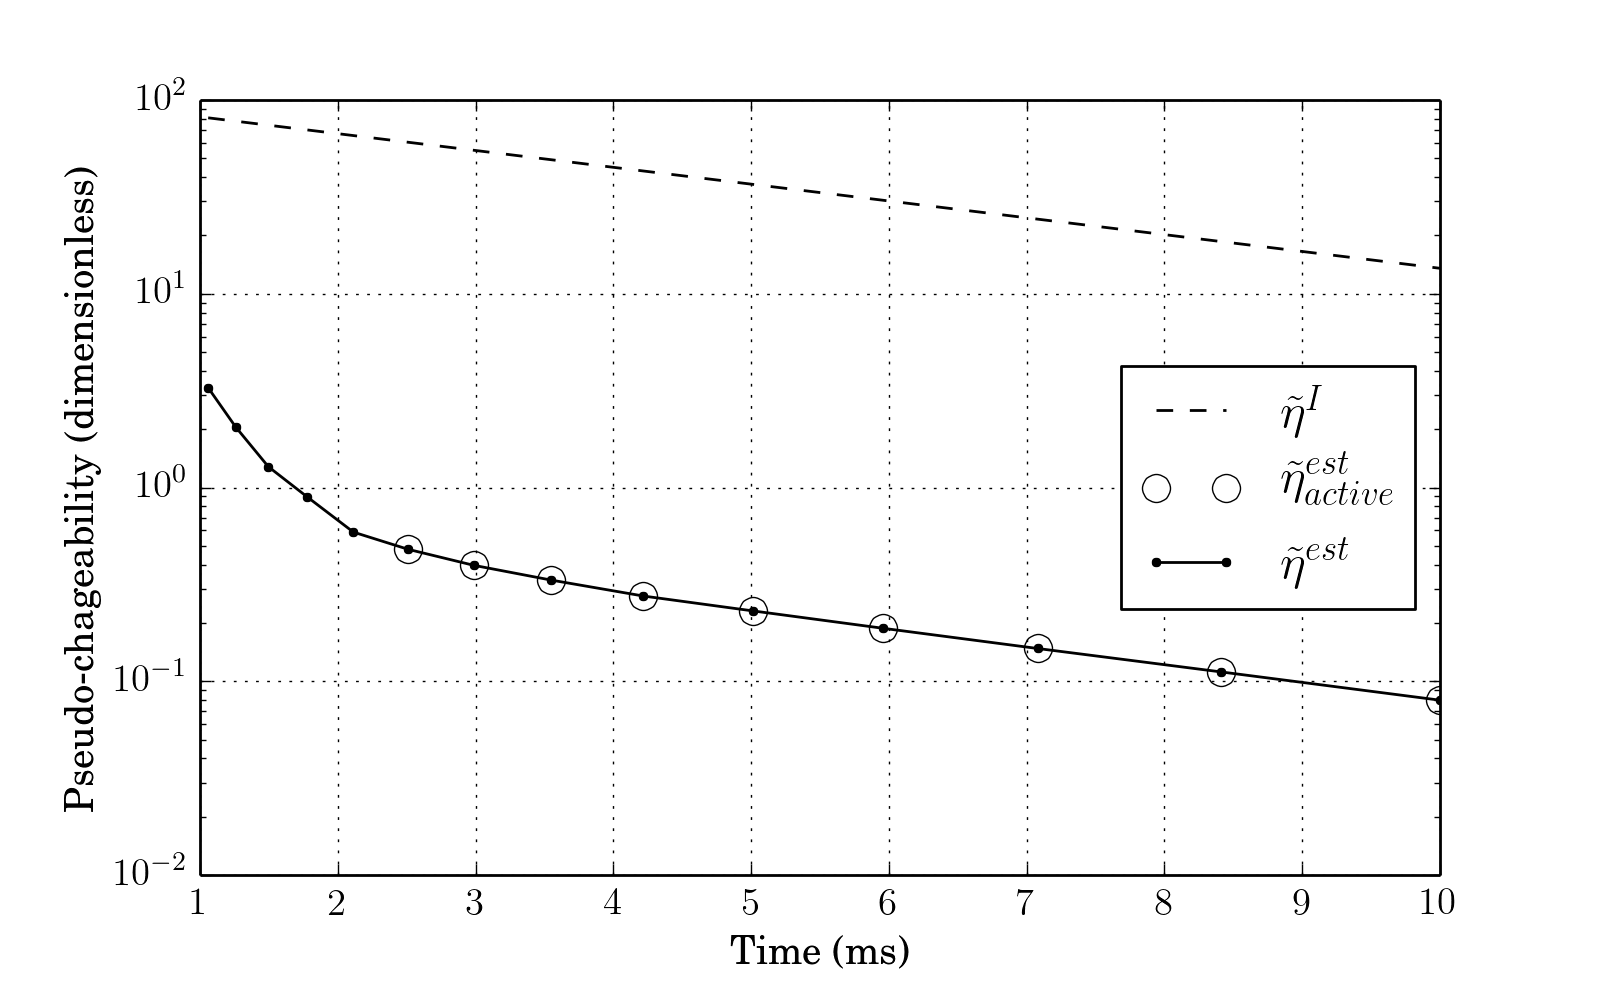
\includegraphics[width=0.8\textwidth]{figures/synthetic/PetaCase2_center.png} \\(b)
  \caption{Time decaying curves of recovered and intrinsic pseudo chargeability at (0, 0, -125). (a) Canonical model. (b) Conductive model. Black dashed and solid line with solid circle indicate $\peta^{I}$ and $\peta^{est}$. Empty circles indicate active set of $\peta^{est}$, which are used to compute slope of time decaying $\peta^{est}$ in semi-log plot. }
  \label{F: Peta_Center}
\end{figure}

\clearpage
\subsection{Field example: Mt. Milligan}
% \subsection{EIP}
% \subsection{MIP}
% \subsection{EM-IP with grounded source}
% \subsection{EM-IP with inductive source (ATEM) }

\clearpage
\section{Appendix}
\subsection{Derivation of the sensitivity   in discretized space}
The numerical evaluation of Maxwell's equations for the steady-state case can be derived by discretizing the system in space using finite volume (FV) method with weak formulation (CITE). For the discretization, we assume that the electric field $\e$ is discretized by grid function $\de$ on cell edges and magnetic flux density $\b$ is discretized by grid fuction $\db$ on cell faces. Electrical potential $\phi$ is discretized by grid fucntion  $\phi$ on cell nodes. For clear representation of the derivation, recall Maxwell's equations in steady state as
\begin{align}
  \j = \sigma\e = -\sigma\grad \phi, \\
  -\div \j = \div \j_s, \\
  \j\big|_{\partial \Omega}\cdot\hat{n} = 0,
  \label{eq:DCBCneumann}
\end{align}
where $\partial \Omega$ indicates boundary surface of the system and $\hat{n}$ is the normal vector of the boundary surface. Modified from CITE, weak form of those equations can be written as
\begin{align}
  (\j, \vec{w}) + (\sigma \grad \phi, \vec{w}) = 0, \\
  -(\j, \grad \psi) = (\j_s, \grad \psi).
\end{align}
The inner products $(\j, \vec{w})$, $(\sigma \grad \phi, \vec{w})$,  $(\j, \grad \psi)$ and $(\j_s, \grad \psi)$ are edge based products. Here we define the inner product as
\begin{equation}
  (\vec{a}, \vec{b}) = \int_{\Omega} \vec{a}\cdot\vec{b} dv,
\end{equation}
where $\Omega$ is the volume of the system. By discretizing $\grad$ operator and the inner product in space, we obtain
\begin{equation}
  \Me\dj + \MeSig\dgrad\phi = 0,
  \label{eq:DCdisceq1}
\end{equation}
\begin{equation}
  -\dgrad^T \Me\dj = \dgrad^T \Me\dj_s,
  \label{eq:DCdisceq2}
\end{equation}
where $\mathbf{M}^e_i$ is the mass matrices, which discretize the edge based inner product (CITE). This inner products are defined  as
\begin{align}
  \mathbf{M}^e_i = \diag(\Ace^T\diag(\vol)\mathbf{i}).
\end{align}
Here, $\mathbf{i}$ indicates a grid function on cell center like $\sigma$, and $\vol$ is the grid function for the cell volume. The averaging matrix $\Ace$ averages discrete function defined on the edges to the cell center. The mass matrix $\Me$ without subscript $i$ indicates that $\mathbf{i}$ is equal to the identity column vector of which all elements are one. By substituting equation (\ref{eq:DCdisceq1}) to (\ref{eq:DCdisceq2}), we have
\begin{equation}
  \A^{DC}\phi = \mathbf{rhs}^{DC},
  \label{eq:DCdiscLin}
\end{equation}
where $\A^{DC} = \dgrad^T \MeSig\dgrad$ and $\mathbf{rhs}^{DC} = \dgrad^T \Me\dj_s$. Sensitivity function of $\phi$ can be derived by taking derivative to equation (\ref{eq:DCdiscLin}) in terms of $\sigma$:
\begin{equation}
  \frac{\partial \phi}{\partial \sigma} = -(\A^{DC})^{-1}\dgrad^T\diag(\dgrad\phi)\Ace^T\diag(\vol).
  \label{eq:DCsensedisc}
\end{equation}
We recall that continuous sensitivity function shown in equation (\ref{eq: senseDC}), which can be modified as
\begin{equation}
  \frac{\partial \phi}{\partial \sigma} = -[\div\sigma\grad]^{-1}\div\grad\phi.
  \label{eq:DCsensecont}
\end{equation}
One can intuitively identify that continuous sensitivity function shown in equation (\ref{eq:DCsensecont}) can be discretized as equation (\ref{eq:DCsensedisc}) with the boundary condition specified on equation (\ref{eq:DCBCneumann}). This approach shows that some advantages of working in discretized space even for the derivation of continuous function (CITE).


\clearpage
\bibliographystyle{plain}
\bibliography{reference}

\end{document}



% http://www.math.mun.ca/tex-archive/macros/latex/contrib/todonotes/todonotes.pdf
